\chapter{Restless Arms with Known TPMs}
\label{ch:restless_with_known_TPMs}

\section{Preamble}
In the previous chapter, we analysed the setting when the arms are rested, i.e., the unobserved arms remain frozen and do not evolve. In this chapter, we analyse the more difficult setting of restless arms in which the unobserved arms continue to evolve.  To begin with, we consider the simpler case when the TPMs are known beforehand. All the essential conceptual difficulties related to the setting of restless arms remain despite this simplification. Formally, given a multi-armed bandit with $K\geq 3$ arms and an arms configuration $C=(h, P_{1}, P_{2})$ in which $h$ is the index of the odd arm, the TPM of arm $h$ is $P_{1}$, and the TPM of each of the remaining arms is $P_{2}\neq P_{1}$, we wish to characterise $$ \lim\limits_{\epsilon\downarrow 0}  \inf\limits_{\pi\in \Pi(\epsilon)} \frac{E^{\pi}[\tau(\pi)|C]}{\log (1/\epsilon)} $$ for the setting of restless arms when $P_{1}$ and $P_{2}$ are known beforehand.

As we shall see later in the chapter, the continued evolution of the Markov process of each arm makes it necessary to keep a record of (a) the time elapsed since each arm was previously selected (called the arm's \emph{delay}), and (b) the state of each arm as observed at its previous selection time (called the \emph{last observed state} of the arm). The notion of arm delays is superfluous when the arms are rested because the unobserved arms remain frozen at their previously observed states. It is superfluous also in the special case of the restless setting when each arm yields iid observations as in the prior works \cite{Vaidhiyan2017, vaidhiyan2012active, vaidhiyan2017learning, prabhu2017learning} because at any given time, the current state of an arm is independent of its last observed state. Therefore, the notions of arm delays and last observed states are strikingly new features of the setting of restless arms. 

\subsection{Motivation and the Notion of a Trembling Hand}
As alluded to in the previous chapters, our motivation to study the problem of odd arm identification in the setting of restless arms comes from the desire to extend the analysis of Vaidhiyan et al. in \cite{Vaidhiyan2017, vaidhiyan2012active, vaidhiyan2017learning} to more general settings. It is often the case in such visual search experiments that though the subject intends to focus his/her attention at a certain location, the actual focus location differs from the intended focus location with a small probability. We model this in our multi-armed bandit setting as a {\em trembling hand} for the decision entity: with probability $1-\eta$, the decision entity samples the intended arm, but with probability $\eta$, the decision entity samples a uniformly randomly chosen arm. Up to Section \ref{restless_with_known_sec:main_result}, we assume that $\eta>0$, as is often the case in visual search experiments such as that described above. The case when $\eta=0$ is dealt with separately in Section \ref{restless_with_known_sec:case_eta_=_0}.

Our assumption about the uniform sampling of the arms under the trembling hand model is merely for convenience, and any probability distribution on the arms that puts a strictly positive mass on each of the arms may be used in place of the uniform distribution. The values of all the expectations and probabilities (in particular, the lower bound of Section \ref{restless_with_known_sec:lower_bound}), which rely on the uniform sampling assumption, will accordingly differ.

For a related example in the cognitive radio setting (no trembling) in which the number of anomalous arms may be more than one, see \cite{zhao2008myopic}.

\subsection{Prior Works on Restless Arms}
The topic of restless arms has been studied extensively in the literature in the context of reward maximisation (or equivalently, regret minimisation). In such works, each arm is assumed to yield, upon being sampled, an immediate `reward' based on the arm's current state. Regret is then defined as the difference between the expected sum of rewards obtained under a particular arm selection scheme and that obtained by a scheme that knows which arm yields the highest expected reward. Whittle \cite{whittle1988restless} 
%is perhaps the first known work that deals with restless arms. Whittle 
refined and extended the results of Gittins \cite{gittins1979bandit} on the optimality, in the setting of rested arms, of a certain index-based policy. Whittle \cite{whittle1988restless} demonstrated that Gittins's policy in \cite{gittins1979bandit} is not necessarily optimal in the context of restless arms, introduced a new index (now called \emph{Whittle's index}) which could be computed if each arm satisfied an \emph{indexability} condition, and demonstrated that the new index coincides with Gittins's index in the rested setting. 
Yet, as Whittle showed, the new index-based policy is not necessarily optimal for the general setting of restless arms.

Whittle's results require the Markov transition laws of each of the arms to be known beforehand. Extensions of Whittle's results to the case when the laws are not known beforehand appear in Liu et al. \cite{liu2012learning}. Ortner et al. \cite{ortner2012regret} provide a policy that, when the transition laws of the arms are unknown, gives a regret of the order $O(\sqrt{T})$ after $T$ time steps in relation to a policy that knows the Markov transition laws of all the arms. As Ortner et al. show in \cite{ortner2012regret}, an optimal policy for the restless bandit problem does not necessarily pick the arm with the largest stationary mean at each time instant\footnote{This is indeed the case in a multi-armed bandit problem with iid observations from each arm, as was shown in \cite{auer2002finite}.}, but instead switches between the arms in an optimal fashion. Working on this key idea, Gr\"unelwalder et al.  \cite{grunewalder2019approximations} provide conditions under which the problem of finding the arm with the largest stationary mean serves as a ``good'' approximation to the original problem of finding the optimal arm switching strategy when each arm is a stationary $\phi$-mixing process and the arms are restless. The works \cite{ortner2012regret} and \cite{grunewalder2019approximations} deal with general state spaces (i.e., not necessarily finite or countable) and address the associated technical challenges.

While the above mentioned works focus on maximising rewards (or equivalently, minimising regret), our focus is on the stopping problem of identifying the index of the odd arm as quickly as possible. For a related problem of best arm identification instead of odd arm identification, see \cite{moulos2019optimal, Kaufmann2016}. The recent works  \cite{deshmukh2018controlled}, \cite{deshmukh2019sequential} and \cite{prabhu2020sequential} deal with more general problems of sequential hypothesis testing in multi-armed bandits, special cases of which are the problems of best arm identification and odd arm identification, in the context of iid observations from each arm. In contrast to these works, we study in this chapter the specific problem of odd arm identification in the more difficult setting of restless arms.

\subsection{A Brief Overview of Our Contributions}
Below, we highlight our contributions and bring out the challenges that we need to overcome in the analysis of the setting of restless arms when the TPMs of the arms are assumed to be known beforehand.
\begin{enumerate}
	\item We show that given a pre-specified error probability threshold $\epsilon>0$, the expected time taken by the decision maker to identify the index of the odd arm with probability of error at most $\epsilon$ grows as $\Theta(\log (1/\epsilon))$. We give a precise characterisation of the best (smallest) constant multiplying $\log (1/\epsilon)$, which we call $R^*(P_1,P_2)$, in terms of the Markov transition probability matrices $P_1$ and $P_2$. This is the first known characterisation of this constant for the setting of restless Markov arms. 
%	\item This result provides a lower bound on the expected time required to identify the index of the odd arm. 
       See Section \ref{restless_with_known_sec:lower_bound} for an exact mathematical expression. 
       We prove this by first showing a lower bound in Section \ref{restless_with_known_sec:lower_bound} and then a matching asymptotic upper bound in Section \ref{restless_with_known_sec:achievability}.
      
     \item An examination of the lower bounds in the prior works \cite{Vaidhiyan2017,vaidhiyan2012active, vaidhiyan2017learning, prabhu2017optimal} reveals that the best constant multiplier in these works is the solution to an optimisation problem having an outer supremum over all (unconditional) probability distributions on the arms, followed by an inner minimum over all alternative odd arm locations (i.e., a sup-min optimisation problem). A further examination reveals that when arm $h$ is the odd arm, there exists a probability distribution $\lambda_h^*$ on the arms, possibly depending on the odd arm location $h$,  that (a) attains the outer supremum, and (b) puts equal mass on each of the non-odd arm locations.
     
      Along lines similar to those of the prior works, we show that the best constant multiplier $R^*(P_1,P_2)$ is the solution to a sup-min optimisation problem in which the supremum is over all \emph{conditional} probability distributions on the arms, conditioned on arm delays and last observed states, and the minimum is over all alternative odd arm locations. We also show that the constant $R^*(P_1,P_2)$ is not a function of the actual odd arm location; this is due to symmetry in the structure of the arms. The constant $R^*(P_1,P_2)$ represents the amount of effort required to identify the true odd arm location by guarding against identifying the nearest, incorrect alternative odd arm location. 
     
     However, given an odd arm location $h$, the question of whether there exists a conditional probability distribution that attains the supremum in the expression for $R^*(P_1,P_2)$ is still under study.
	
	\item In order to derive the constant $R^*(P_1,P_2)$, we use the fact that the arm delays and the last observed states form a \emph{controlled Markov process}, with the arm selections playing the role of \emph{controls}. This approach of ours takes into account the delays and the last observed states of \emph{all} the arms jointly. In contrast, the approaches of \cite{Vaidhiyan2017,vaidhiyan2012active, vaidhiyan2017learning, prabhu2017optimal}  suggest dealing with the delays and the last observed states of each of the arms separately, which we view as a `local' perspective of the arm delays and the last observed states. In Section \ref{restless_with_known_appndx:infinite_dimensional_LP}, we show that this local perspective of arm delays and last observed states leads to an infinite dimensional, constrained, linear programming problem (LPP). The drawback of this approach is that it is not easy to find the tightest set of constraints for the LPP. As a consequence, the constant multiplier obtained as the solution to the LPP may not necessarily be the best (smallest). 
	
	On the other hand, our `lift' approach, which considers the delays and the last observed states of all the arms jointly, leads us naturally to a family of Markov decision problems (MDPs) and, in turn, provides the necessary perspective to arrive at the best constant multiplier $R^*(P_1,P_2)$.
	
	\item We show that under a \emph{stationary} arm selection policy (in which at each time, the arms are selected according to a certain conditional probability distribution on the arms, conditioned on the delays and last observed states at that time), the aforementioned controlled Markov process is, in fact, a Markov process. Additionally, we show that under every stationary arm selection policy, this Markov process is \emph{ergodic} when the trembling hand parameter $\eta>0$ (Lemma \ref{restless_with_known_lem:pi_delta^lambda_is_an_SSRS}). It is this ergodicity property, together with the strict positivity of the trembling hand parameter $\eta$, that plays a crucial role in our analysis of the lower and the upper bounds. The case $\eta=0$ demands a careful examination since, in this case, such an ergodicity property is not readily available for every stationary arm selection policy. 	
	\item We show that for every arm selection policy of the decision maker, stationary or otherwise, what enters into the analyses of the lower and the upper bounds is the following statistic: for each possible value of arm delays $\underline{d}$, last observed states $\underline{i}$ and arm $a$, the long-term fraction of times the aforementioned controlled Markov process visits the state $(\underline{d},\underline{i})$ and arm $a$ is selected.  
	This fact, together with Theorem \ref{restless_with_known_theorem:restriction_to_SRS_policies}, enables us to restrict attention only to stationary arm selection policies in arriving at the best constant multiplier $R^*(P_1,P_2)$.  
	
	In spite of the above simplification, the computability of $R^*(P_1,P_2)$ remains an issue since it involves a search over the space of all stationary arm selection policies. One must resort to \emph{Q}-learning in the context of restless Markov arms (see, for instance, \cite{avrachenkov2020whittle}) to compute $R^*(P_1,P_2)$. {\color{black} Under some circumstances, good approximations to $R^*(P_1, P_2)$ may be possible; see Section \ref{restless_with_known_sec:conclusions}.}
	
	\item The question of whether the supremum in the expression for $R^*(P_1,P_2)$ is attainable is still under study, as mentioned in point 2 above. The arm delays, being positive and integer-valued, introduce a countably infinite dimension to the problem. As a consequence, it is not clear if the space of all conditional distributions on the arms, conditioned on the arm delays and the last observed states, is compact. In the iid and the rested Markov settings of the prior works, only unconditional distributions on the arms appear in the analysis of the lower and the upper bounds, and because of the finite nature of the number of arms, it follows immediately that the space of all unconditional distributions on the arms is compact. Such a compactness property plays a key role in showing that the supremum is attained.
	
	Notwithstanding the additional technical difficulty encountered in the setting of restless arms due to the presence of the countably infinite-valued arm delays, we show that the supremum in the expression for $R^*(P_1, P_2)$ may be approached arbitrarily closely by stitching together certain parameterised solutions to the MDPs mentioned in point 3 above. We present the details in Section \ref{restless_with_known_sec:achievability}.
		
    \item The trembling hand model (with $\eta>0$) may be viewed as a regularisation that ensures stability of the aforementioned controlled Markov process (of arm delays and last observed states) for free. If $\eta=0$, one could deliberately add some regularisation parameterised by $\eta$, re-label the constant $R^*(P_1,P_2)$ in this case as $R_\eta^*(P_1,P_2)$ for each $\eta>0$, and analyse the limiting value of $R_\eta^*(P_1,P_2)$ as $\eta\downarrow 0$. We show that in this case, (a) the limit of $R_\eta^*(P_1,P_2)$ as $\eta\downarrow 0$ exists, and (b) the upper bound is governed by $\lim\limits_{\eta\downarrow 0}R_\eta^*(P_1,P_2)$, while the lower bound is governed by $R_0^*(P_1,P_2)$ (which is obtained by plugging $\eta=0$ in the expression for $R_\eta^*(P_1,P_2)$). So, the question then is, do these lower and the upper bounds match? In Section \ref{restless_with_known_sec:case_eta_=_0}, we are only able to establish that $\lim\limits_{\eta\downarrow 0}R_\eta^*(P_1,P_2)\leq R_0^*(P_1,P_2)$. A key tool needed to establish equality in this inequality is the ``envelope theorem'' \cite[Theorem 2]{milgrom2002envelope}. A verification of the hypotheses of the envelope theorem for the setting of restless arms still remains open.
    
	\item We verify that the envelope theorem holds in the iid and rested Markov settings of the prior works \cite{Vaidhiyan2017,vaidhiyan2012active, vaidhiyan2017learning, prabhu2017optimal}, thus leading to matching upper and lower bounds in these works. Thus, sufficient conditions for the upper and the lower bounds to match are either (a) $\eta>0$, or (b) $\eta=0$ and the observations come from either iid or rested Markov arms.
\end{enumerate}

\subsection{Chapter Organisation}
The rest of this chapter is organised as follows. In Section \ref{restless_with_known_sec:notations}, we set up the notations and provide some preliminaries that will be useful for the rest of the chapter. 
%In Section \ref{restless_with_known_sec:ergodicity_lemma}, we present an important lemma on the ergodicity of the controlled Markov process of arm delays and last observed states. 
In Section \ref{restless_with_known_sec:lower_bound}, we present the lower bound on {\color{black} the growth rate of} the expected time to find the odd arm as a function of the error probability. In the same section, we also show that by following the conventional approaches available in the prior works, we arrive at an infinite-dimensional linear programming problem (LPP) with countably infinitely many constraints that is difficult to solve. In Section \ref{restless_with_known_sec:achievability}, we present a sequence of strategies whose expected times to find the index of the odd arm approach the lower bound in the limit of vanishing error probabilities, following which we state the main result of this chapter in Section \ref{restless_with_known_sec:main_result}. We discuss the no trembling hand case in Section \ref{restless_with_known_sec:case_eta_=_0}. 
%We present some remarks on the existence of optimal arm selection policies in Section \ref{restless_with_known_sec:existence_of_optimal_policies}. 
The proofs of all the results are contained in Section \ref{restless_with_known_sec:proofs}. Section \ref{restless_with_known_appndx:an_important_theorem} contains the statement of an important theorem that is used in several places in the main body of the chapter.

\section{Notations and Preliminaries}
\label{restless_with_known_sec:notations}
As in the previous chapter, we consider a multi-armed bandit with $K\geq 3$ arms, and define $\mathcal{A}\coloneqq \{1,\ldots,K\}$ to be the set of arms. We associate with each arm an ergodic and discrete-time Markov process on a finite state space $\mathcal{S}$. Further, we assume that the Markov process of any given arm is independent of those of the other arms. The Markovian evolution of states on one of the arms (known as the \emph{odd} arm) is governed by a transition probability matrix $P_1$, and the evolution of states on each of the non-odd arms is governed by $P_2$, where $P_2\neq P_1$. We denote by $\mu_i$ the unique stationary distribution of $P_i$, $i=1,2$.

For any integer $d\geq 1$ and a transition probability matrix $P$ on $\mathcal{S}$, let $P^{d}$ denote the transition probability matrix obtained by multiplying $P$ with itself $d$ times. For $i,j\in\mathcal{S}$ and $d\geq 1$, we write $P_1^{d}(j|i)$ and $P_{2}^{d}(j|i)$ to denote the $(i,j)$th element of the matrices $P_1^{d}$ and $P_{2}^{d}$ respectively (the case $d=1$ corresponds to $P_{1}$ and $P_{2}$ respectively). We assume that for all $i,j\in\mathcal{S}$, (a) $P_1(j|i)>0$ if and only if $P_2(j|i)>0$. This assumption ensures that the decision maker cannot infer whether or not a given arm is the odd arm merely by observing certain specific state(s) or state-transition(s) on the arm. For $h\in\mathcal{A}$, we denote by $\mathcal{H}_h$ the hypothesis that $h$ is the odd arm location.

We assume that $P_1$ and $P_2$ are known to a decision maker, whose goal it is to identify the index of the odd arm as quickly as possible, subject to an upper bound on the probability of error. In order to do so, the decision maker devises a sequential arm selection strategy in which, at each discrete-time instant $t\in\{0,1,\ldots\}$, the decision maker first identifies an arm to pull; call this $B_{t}$. The decision maker however has a trembling hand and, as a consequence, the intended arm $B_{t}$ gets pulled with probability $1-\eta$ and a uniformly random arm gets pulled with probability $\eta$. The parameter $\eta$, which is fixed and strictly positive, governs the error in translating the decision maker's intention into an action. Write $A_{t}$ for the arm that is actually pulled. The decision maker observes $A_{t}$, therefore knows whether or not his hand made an error in pulling the intended arm. Further, the decision maker observes the state of the arm $A_{t}$, denoted by $\bar{X}_{t}$. The unobserved arms continue to undergo state evolution, making the arms \emph{restless}. Thus, for each $t\geq 0$, $B_{t}, A_{t}$ and $\bar{X}_{t}$ denote respectively the intended arm, the selected arm, and the observed state of the selected arm at time $t$. We use the shorthand notation $(B^{t}, A^{t},\bar{X}^{t})$ to denote the collection $(B_0,A_0,\bar{X}_0,\ldots,B_{t},A_{t}\,\bar{X}_{t})$.

{\color{black} We note here that the observations $\{\bar{X}_t: t\geq 0\}$ are noiseless. The case of noisy observations, e.g., hidden Markov models, is important and is left for future work.}

\subsection{Policy}
A policy prescribes one of the following two actions at each time $t$: Based on the history $(B^{t-1},A^{t-1},\bar{X}^{t-1})$,
\begin{itemize}
	\item choose to pull arm $B_t$ according to a deterministic or a randomised rule, or
	\item stop and declare the index of the odd arm.
\end{itemize}
We use $\pi$ to denote a generic policy, and let $\tau(\pi)$ denote the stopping time of policy $\pi$. Throughout this chapter, all stopping times are defined with respect to the filtration $\mathcal{F}_t\coloneqq\sigma(B^{t-1},A^{t-1},\bar{X}^{t-1})$, $t\geq 1$ and $\mathcal{F}_{0}\coloneqq \{\Omega,\emptyset\}$. Let $\theta(\tau(\pi))$ denote the index of the odd arm declared by the policy $\pi$ at its stopping time $\tau(\pi)$.

Let $P_h^\pi(\cdot)$ and $E_h^\pi[\cdot]$ denote probabilities and expectations computed under policy $\pi$. For ease of notation, we drop the superscript $\pi$, and {\color{black} request the  reader} to bear the dependence on $\pi$ in mind. Given a target probability of error $\epsilon>0$, we define $\Pi(\epsilon)$ as the set
\begin{equation}
	\Pi(\epsilon)\coloneqq \{\pi:P_h(\theta(\pi)\neq h)\leq \epsilon\text{ for all }h\in\mathcal{A}\}\label{restless_with_known_eq:Pi(epsilon)}
\end{equation}
of all policies whose probability of error at stoppage is below $\epsilon$ {for all possible odd arm locations}. We emphasise that policies in $\Pi(\epsilon)$ work for all possible odd arm locations. We anticipate from similar results in the prior works that $$\inf\limits_{\pi\in\Pi(\epsilon)}E_h[\tau(\pi)] = \Theta(\log(1/\epsilon)).$$
Our interest is in characterising the constant factor multiplying $\log(1/\epsilon)$ {\color{black} in the limit as $\epsilon\downarrow 0$. For simplicity, we assume that every policy starts with the observation that arm $1$ is observed at time $t=0$, arm $2$ is observed at time $t=1$, etc., and arm $K$ is observed at time $t=K-1$. This can be effected by sampling the arms uniformly until this event occurs. Clearly, for $\eta > 0$, this requirement will result in a finite delay almost surely which does not affect the asymptotic analysis as $\epsilon \downarrow 0$.}

\subsection{Delays and Last Observed States}
Recall that at each time $t\in \{0,1,\ldots\}$, the decision maker observes only one of the arms, while the unobserved arms continue to undergo state evolution. Therefore, the probability of the observation $\bar{X}_t$ on the {selected} arm $A_t$ is a function of (a) the time elapsed since the previous time instant of selection of arm $A_t$ (called the \emph{delay} of arm $A_t$), and (b) the state of arm $A_t$ at its previous selection time instant (called the \emph{last observed state} of arm $A_t$). Notice that when the arms are \emph{rested}, the notion of arm delays is superfluous since each arm remains frozen at its previously observed state until its next selection time instant. Also, the notion of arm delays is redundant in the setting of iid observations since, in this special case, the current state of the arm selected is independent of the state at its previous selection. Thus, the notion of arm delays is a key distinguishing feature of the setting of restless arms.

We now define a new and more convenient notion of a state, based on the delays and the last observed states of the arms. As we demonstrate below, this new notion of state results in a  Markov decision problem that is amenable to analysis.

For $t\geq K$, we denote by $d_a(t)$ and $i_a(t)$ respectively the delay and the last observed state of arm $a$ at time $t$. Write $\underline{d}(t) \coloneqq (d_1(t),\ldots,d_K(t))$ and $\underline{i}(t) \coloneqq (i_1(t),\ldots,i_K(t))$ for the delays and the last observed states, respectively, of the arms at time $t$. Note that arm delays and last observed states are defined only for $t\geq K$ since these quantities are well-defined only when at least one observation is available from each arm. We set $\underline{d}(K)=(K,K-1,\ldots,1)$. {\color{black} Thus, we observe that $d_a(t)\geq 1$ for all $t\geq K$, and that $d_a(t)=1$ if and only if arm $a$ is selected at time $t-1$}.

We follow the rule below for updating the arm delays and last observed states: if $A_{t}=a'$, then
\begingroup \allowdisplaybreaks\begin{align}
	{d}_a(t+1)=\begin{cases}
		d_a(t)+1, &a\neq a',\\
		1,& a=a',
	\end{cases} \qquad \qquad 
	i_a(t+1)=\begin{cases}
		i_a(t),& a\neq a',\\
		\bar{X}_{t},& a=a',
	\end{cases}
	\label{restless_with_known_eq:specific_transition_pattern}
\end{align}\endgroup
where $\bar{X}_{t}$ is the state of the arm $A_t=a'$ at time $t$.

One thus has the sequence of intended arm pulls, actual arm pulls, observations, and states as follows: at each $t \geq K$, based on $(\underline{d}(t), \underline{i}(t))$, choose to pull $B_{t}$; due to the trembling hand, observe that $A_{t}$ is pulled; see the state $\bar{X}_{t}$ of arm $A_t$; then form $(\underline{d}(t+1), \underline{i}(t+1)) $. This repeats until stoppage, at which time we have the declaration $\theta(\tau(\pi))$ (under policy $\pi$) as the candidate odd arm.

\subsection{Controlled Markov Process and the Resulting Markov Decision Problem}
From the update rule in \eqref{restless_with_known_eq:specific_transition_pattern}, it is clear that the process $\{(\underline{d}(t),\underline{i}(t)):t\geq K\}$ takes values in a subset $\mathbb{S}$ of the {countable} set $\mathbb{N}^K\times\mathcal{S}^K$, where $\mathbb{N}=\{1,2,\ldots\}$ denotes the set of natural numbers. The subset $\mathbb{S}$ is formed based on the constraint that at any time $t\geq K$, exactly one of the components of $\underline{d}(t)$ is equal to $1$, and all the other components are {\color{black} $>1$}. Note that for all $(\underline{d},\underline{i}) \in \mathbb{S}$ and $t\geq K$,
\begin{align}
	&P(\underline{d}(t+1)=\underline{d},\underline{i}(t+1)=\underline{i}\mid (\underline{d}(s),\underline{i}(s)),B_s,~K\leq s\leq t)\nonumber\\
	&=P(\underline{d}(t+1)=\underline{d},\underline{i}(t+1)=\underline{i}\mid (\underline{d}(t),\underline{i}(t)),B_t).\label{restless_with_known_eq:controlled_markov_chain}
\end{align}
On account of \eqref{restless_with_known_eq:controlled_markov_chain} being satisfied, we say that under any policy $\pi$, the evolution of the process $\{(\underline{d}(t),\underline{i}(t)):t\geq K\}$ is \emph{controlled} by the sequence $\{B_t\}_{t\geq 0}$ of intended arm selections under policy $\pi$. Alternatively, we say that $\{(\underline{d}(t),\underline{i}(t)):t\geq K\}$ is a controlled Markov process, with $\{B_t\}_{t\geq 0}$ as the sequence of controls; the terminology used here follows that of Borkar \cite{borkar1988control}. Thus, we are in a Markov decision problem (MDP) setting. We now make precise the state space, the action space, the transition probabilities and our objective.

The state space of the MDP is $\mathbb{S}$, with the state at time $t$ denoted $(\underline{d}(t), \underline{i}(t))$. The action space of the MDP is $\mathcal{A}$, with action $B_t$ at time $t$ possibly depending on the previous actions $B^{t-1}$ and the previous states $\{(\underline{d}(s), \underline{i}(s)), K \leq s \leq t\}$. (It is easy to see that this is equivalent to taking an action based on $(B^{t-1}, A^{t-1}, \bar{X}^{t-1})$.) The transition probabilities for the MDP are given by
\begin{enumerate}
	\item the trembling hand rule
\begin{equation}
	P(A_t = a | B_t) = \frac{\eta}{K}+ (1-\eta) \,\,\mathbb{I}_{\{B_t = a\}}, \quad \forall a \in \mathcal{A},\label{restless_with_known_eq:trembling_hand_rule}
\end{equation}
	\item the law associated with arm $A_t$, and
	\item the update rule \eqref{restless_with_known_eq:specific_transition_pattern}.
\end{enumerate}
In \eqref{restless_with_known_eq:trembling_hand_rule}, $\mathbb{I}$ denotes the indicator function. In order to write the transition probabilities of the MDP precisely, let us introduce some notations. Given $h,a\in\mathcal{A}$, let $P_h^a$ denote the transition probability matrix of the Markov process of arm $a$ under the hypothesis $\mathcal{H}_h$. That is,
\begin{equation}
	P_h^a=\begin{cases}
		P_1,&a=h,\\
		P_2,&a\neq h.
	\end{cases}\label{restless_with_known_eq:P_h^a}
\end{equation}
Furthermore, for any integer $d\geq 1$, let $(P_h^a)^d$ denote the transition probability matrix obtained by multiplying $P_h^a$ with itself $d$ times. Then, given any $(\underline{d},\underline{i}), (\underline{d}',\underline{i}')\in\mathbb{S}$ and $b\in\mathcal{A}$, the transition probabilities for the MDP are given by 
\begin{align}
	&P(\underline{d}(t+1)=\underline{d}',\underline{i}(t+1)=\underline{i}'\mid \underline{d}(t)=\underline{d},\underline{i}(t)=\underline{i}, B_t=b)\nonumber\\
	&=\begin{cases}
		\left(\frac{\eta}{K}+(1-\eta)\,\mathbb{I}_{\{b\}}(a)\right)\,(P_h^a)^{d_a}(i_a'|i_a),&\text{if }d_a'=1\text{ and }d'_{\tilde{a}}=d_{\tilde{a}}+1\text{ for all }\tilde{a}\neq a,\\
		&i_{\tilde{a}}'=i_{\tilde{a}}\text{ for all }\tilde{a}\neq a,\\
		0,&\text{otherwise},
	\end{cases}\label{restless_with_known_eq:MDP_transition_probabilities}
\end{align}
where $d_a'$ and $i_a'$ in \eqref{restless_with_known_eq:MDP_transition_probabilities} denote the component corresponding to arm $a$ in $\underline{d}'$ and $\underline{i}'$ respectively. Note that the transition probabilities defined in \eqref{restless_with_known_eq:MDP_transition_probabilities} are stationary and independent of time. Also, for $a\in \mathcal{A}$, we have
\begin{align}
	&P(\underline{d}(t+1)=\underline{d}',\underline{i}(t+1)=\underline{i}'\mid \underline{d}(t)=\underline{d},\underline{i}(t)=\underline{i}, A_t=a)\nonumber\\
	&\hspace{4cm}=\begin{cases}
		(P_h^a)^{d_a}(i_a'|i_a),&\text{if }d_a'=1\text{ and }d_{\tilde{a}}'=d_{\tilde{a}}+1\text{ for all }\tilde{a}\neq a,\\
		&i_{\tilde{a}}'=i_{\tilde{a}}\text{ for all }\tilde{a}\neq a,\\
		0,&\text{otherwise}.
	\end{cases}\label{restless_with_known_eq:MDP_transition_probabilities_A_t}
\end{align}
The left-hand sides of \eqref{restless_with_known_eq:MDP_transition_probabilities} and \eqref{restless_with_known_eq:MDP_transition_probabilities_A_t} differ in that $B_t$ in \eqref{restless_with_known_eq:MDP_transition_probabilities} is replaced by $A_t$ in \eqref{restless_with_known_eq:MDP_transition_probabilities_A_t}. We shall write $Q(\underline{d}',\underline{i}'|\underline{d},\underline{i},a)$ to denote the quantity in \eqref{restless_with_known_eq:MDP_transition_probabilities_A_t}.

Our objective, however, is nonstandard in the context of MDPs, and more in line with what information theorists study. We are interested in determining, for each hypothesis $\mathcal{H}_h$, the following:
\begin{equation}
  \label{restless_with_known_eqn:objective}
  \lim_{\epsilon \downarrow 0} ~ \inf_{\pi \in \Pi(\epsilon)} ~ \frac{E_h [\tau(\pi)]}{\log (1/\epsilon)}.
\end{equation}

In the next section, we provide some preliminaries on MDPs. The terminologies used follow Borkar \cite{borkar1988control}.

\section{Preliminaries on MDPs}\label{restless_with_known_sec:MDP_preliminaries}
Let $\pi$ be an arbitrary policy. Consider the controlled Markov process $\{(\underline{d}(t),\underline{i}(t)):t\geq K\}$, with the corresponding sequence of controls $\{B_t\}$, under the policy $\pi$. Note that for all $t\geq K$,
\begin{align}
	&P(\underline{d}(t+1)=\underline{d},\underline{i}(t+1)=\underline{i}\mid B^{t-1}, \{(\underline{d}(s),\underline{i}(s)),~K\leq s\leq t\})\nonumber\\
	&=\sum\limits_{b=1}^{K}\bigg[P(B_t=b\mid B^{t-1}, \{(\underline{d}(s),\underline{i}(s)),~K\leq s\leq t\})\nonumber\\
	&\hspace{3cm} \cdot P(\underline{d}(t+1)=\underline{d},\underline{i}(t+1)=\underline{i}\mid B_t=b, ~B^{t-1}, \{(\underline{d}(s),\underline{i}(s)),~K\leq s\leq t\})\bigg]\nonumber\\
	&=\sum\limits_{b=1}^{K}\bigg[P(B_t=b\mid B^{t-1},\{(\underline{d}(s),\underline{i}(s)),~K\leq s\leq t\})\nonumber\\
	&\hspace{5cm}\cdot P(\underline{d}(t+1)=\underline{d},\underline{i}(t+1)=\underline{i}\mid (\underline{d}(t),\underline{i}(t)), B_t=b)\bigg],\label{restless_with_known_eq:completely_specify_transition}
\end{align}
where the last line above follows from \eqref{restless_with_known_eq:controlled_markov_chain}. From \eqref{restless_with_known_eq:completely_specify_transition}, it is evident that the policy $\pi$ may be described completely by specifying  $P(B_{t} | B^{t-1}, \{ (\underline{d}(s),\underline{i}(s)),K\leq s\leq t \})$ for all $t\geq K$. 
%While the choice of arm $B_t$ at time $t$ may potentially depend on the history $\{B^{t-1},\{(\underline{d}(s),\underline{i}(s):K\leq s\leq t\}\}$, it is often the case in practice (for e.g., in visual search experiments such as those described in Section \ref{sec:introduction}) that the choice of arm $B_t$ is based only on the current state $(\underline{d}(t),\underline{i}(t))$ of the underlying controlled Markov process for all $t\geq K$. For the remainder of this chapter, we assume that under every policy $\pi$ of the decision maker, the control sequence $\{B_t\}$ satisfies the aforementioned property. Such control sequences are the most general class of control sequences considered in \cite{borkar1988control} and related works on controlled Markov processes.
We say that a policy $\pi$ is a \emph{stationary randomised strategy} (SRS) if there exists a Cartesian product $\lambda$ of the form
\begin{equation}
	\lambda=\bigotimes \limits_{(\underline{d},\underline{i})\in\mathbb{S}} \lambda_{(\underline{d},\underline{i})},\label{restless_with_known_eq:SRS_Phi_defn}
\end{equation}
with the component $\lambda_{(\underline{d},\underline{i})}(\cdot)$ being a probability measure on $\mathcal{A}$, such that for all $t\geq K$ and $b\in\mathcal{A}$, under the policy $\pi$,
\begin{equation*}
	P(B_{t} = b\mid B^{t-1}, \{ (\underline{d}(s),\underline{i}(s)),K\leq s\leq t \})=\lambda_{(\underline{d}(t),\underline{i}(t))}(b).\label{restless_with_known_eq:prob_of_arm_selection_under_SRS_Phi}
\end{equation*}
Such an SRS $\pi$ will be denoted $\pi^{\lambda}$. Note that $\{(\underline{d}(t),\underline{i}(t)):t\geq K\}$ is indeed a \emph{Markov process} under the SRS $\pi^{\lambda}$. This follows from the relation \eqref{restless_with_known_eq:completely_specify_transition} where the first probability term inside the summation in \eqref{restless_with_known_eq:completely_specify_transition} is now a function only of $(\underline{d}(t),\underline{i}(t))$. Let $\Pi_{\textsf{SRS}}$ denote the set of all SRS policies. 

%\begin{remark}
%	For the rest of this chapter, all policies of interest to us will be those belonging to $\Pi_{\textsf{SRS}}$. In particular, we shall view the set $\Pi(\epsilon)$ defined in \eqref{restless_with_known_eq:Pi(epsilon)} as a subset of $\Pi_{\textsf{SRS}}$ for every $\epsilon>0$. In other words, for every $\epsilon>0$, we look for SRS policies whose probability of error at stoppage is below $\epsilon$.
%\end{remark}

For convenience, we write $\lambda_{(\underline{d},\underline{i})}(\cdot)$ as $\lambda(\cdot | \underline{d},\underline{i})$ so that we may write $\lambda$ itself in the more familiar form $\lambda(\cdot | \cdot)$.

An immediate and important property of any $\pi^\lambda\in\Pi_{\textsf{SRS}}$ is the following.

\begin{lemma}\label{restless_with_known_lem:pi_delta^lambda_is_an_SSRS}
Let $\eta\in(0,1]$. For every $\pi^{\lambda}\in\Pi_{\textsf{SRS}}$, the controlled Markov process $\{\underline{d}(t),\underline{i}(t):t\geq K\}$ under the policy $\pi^{\lambda}$ is irreducible, aperiodic, positive recurrent, and hence ergodic.
\end{lemma}
\begin{proof}
See Section \ref{restless_with_known_appndx:proof_of_lemma_pi_delta^lambda_is_an_SSRS}.
\end{proof}
The proof of Lemma \ref{restless_with_known_lem:pi_delta^lambda_is_an_SSRS}  relies on the hypothesis that the trembling hand parameter $\eta>0$. 

As a consequence of Lemma \ref{restless_with_known_lem:pi_delta^lambda_is_an_SSRS}, it follows that under every SRS policy, a unique stationary distribution exists for the Markov process $\{(\underline{d}(t),\underline{i}(t)):t\geq K\}$. Let us call this stationary distribution $\mu^\lambda$ corresponding to the SRS policy $\pi^\lambda$.

With the above ingredients in place, we state in the next section the first main result of this chapter -- an asymptotic lower bound on {\color{black} the growth rate of} the expected time to identify the odd arm. 

%\section{An Important Ergodicity Lemma}
%\label{restless_with_known_sec:ergodicity_lemma}
%\begin{lemma}\label{restless_with_known_lem:pi_delta^lambda_is_an_SSRS}
%Under every SRS policy $\pi^{\lambda}$, the controlled Markov process $\{(\underline{d}(t),\underline{i}(t)):t\geq K\}$ is irreducible, aperiodic, positive recurrent, and hence ergodic.
%\end{lemma}
%\begin{proof}
%See Section \ref{restless_with_known_appndx:proof_of_lemma_pi_delta^lambda_is_an_SSRS}.
%\end{proof}
%The proof of lemma \ref{restless_with_known_lem:pi_delta^lambda_is_an_SSRS}  relies on the hypothesis that the trembling hand parameter $\eta>0$. 
%
%As a consequence of lemma \ref{restless_with_known_lem:pi_delta^lambda_is_an_SSRS}, it follows that under every SRS policy, a unique stationary distribution exists for the Markov process $\{(\underline{d}(t),\underline{i}(t)):t\geq K\}$. Let us call this stationary distribution $\mu^\lambda$ corresponding to the SRS policy $\pi^\lambda$.

\section{Converse: Lower Bound}\label{restless_with_known_sec:lower_bound}
We now present a lower bound for \eqref{restless_with_known_eqn:objective}.
\begin{prop}
    \label{restless_with_known_prop:lower_bound}
	Fix $h\in\mathcal{A}$, and assume that $\mathcal{H}_h$ is the true hypothesis. Let $P_1$ be the transition probability matrix of the Markov process of arm $h$, and for each $a\neq h$, let $P_2$ be the transition probability matrix of the Markov process arm $a$. Then,
\begin{equation}
	\liminf\limits_{\epsilon\downarrow 0}\inf\limits_{\pi\in\Pi(\epsilon)}\frac{E_h[\tau(\pi)]}{\log(1/\epsilon)}\geq \frac{1}{R^*(P_1,P_2)},\label{restless_with_known_eq:lower_bound}
\end{equation}
where $R^*(P_1,P_2)$ is given by
\begingroup \allowdisplaybreaks\begin{align}
R^*(P_1,P_2)
\coloneqq \sup\limits_{\pi^\lambda\in\Pi_{\textsf{SRS}}}\, \min\limits_{h'\neq h} ~ \sum\limits_{(\underline{d},\underline{i})\in\mathbb{S}}~\sum\limits_{a=1}^{K}  \nu^\lambda(\underline{d},\underline{i},a) \,\textcolor{black}{k_{hh'}(\underline{d}, \underline{i}, a)},\label{restless_with_known_eq:R_delta^*(h,P_1,P_2)}
\end{align}\endgroup
with
\begin{equation}
	\textcolor{black}{k_{hh'}(\underline{d}, \underline{i}, a)}\coloneqq
	\begin{cases}
		D(P_1^{d_a}(\cdot|i_a)\|P_2^{d_a}(\cdot|i_a)),&a=h,\\
		{D(P_2^{d_a}(\cdot|i_a)\|P_1^{d_a}(\cdot|i_a))},&a=h',\\
		0,& a\neq h,h',
	\end{cases}\label{restless_with_known_eq:k(a,d_a,i_a)}
\end{equation}
and
\begin{eqnarray}
 \nu^\lambda(\underline{d},\underline{i},a)\coloneqq \mu^\lambda(\underline{d},\underline{i})\left(\frac{\eta}{K}+(1-\eta)\,\lambda(a|\underline{d},\underline{i})\right), \quad
\forall (\underline{d},\underline{i},a)\in\mathbb{S}\times\mathcal{A}.
\label{restless_with_known_eq:ergodic_state_action_occupancy_measure}
\end{eqnarray}
\end{prop}
\begin{proof}
See Section \ref{restless_with_known_appndx:proof_of_prop_lower_bound}.
\end{proof}
The proof of the lower bound follows the outline in \cite{Kaufmann2016}, with necessary modifications for the setting of restless arms. The key ingredients are the data processing inequality for relative entropies, a Wald-type Lemma for Markov processes, and a recognition that, for any $(\underline{d},\underline{i})$, the long-term fraction of exits from the state $(\underline{d},\underline{i})$ matches the long-term fraction of entries into the state $(\underline{d},\underline{i})$. This forces the long-term probability of seeing the controlled Markov process $\{(\underline{d}(t), \underline{i}(t)): t\geq K\}$ in the state $(\underline{d},\underline{i})$ to be that under its unique stationary distribution, by ergodicity (Lemma \ref{restless_with_known_lem:pi_delta^lambda_is_an_SSRS}). These observations lead to  \eqref{restless_with_known_eq:lower_bound}.

Observe that the left-hand side of \eqref{restless_with_known_eq:lower_bound} is evaluated by taking into consideration \emph{all} policies, including those that are not necessarily SRS policies, whereas the supremum in \eqref{restless_with_known_eq:R_delta^*(h,P_1,P_2)} is only over SRS policies. This is a consequence of \cite[Theorem 8.8.2]{puterman2014markov}, a formal statement of which appears in Theorem \ref{restless_with_known_theorem:restriction_to_SRS_policies} of Section \ref{restless_with_known_appndx:an_important_theorem} as applicable to the context of this chapter. For details on how Theorem \ref{restless_with_known_theorem:restriction_to_SRS_policies} is used in the proof, see Section \ref{restless_with_known_appndx:proof_of_prop_lower_bound}. 

Finally, note that the constant $R^*(P_1,P_2)$ in \eqref{restless_with_known_eq:R_delta^*(h,P_1,P_2)} does not depend on the odd arm location $h$. This is due to symmetry in the structure of the arms.

\subsection{Our `Lift' Approach}
It may be a little surprising to the reader as to why the summation on the right-hand side of \eqref{restless_with_known_eq:R_delta^*(h,P_1,P_2)} is over the delays and the last observed states of \emph{all} the arms when the function $\textcolor{black}{k_{hh'}(\underline{d}, \underline{i}, a)}$, as given in \eqref{restless_with_known_eq:k(a,d_a,i_a)}, is a function only of $d_a$ and $i_a$, the delay and the last observed state of arm $a$. In fact, the prior works  \cite{Vaidhiyan2017, vaidhiyan2012active, vaidhiyan2017learning, prabhu2017optimal} suggest that it suffices to use $(d_a, i_a)$ in place of $(\underline{d}, \underline{i})$ for deriving the lower bound. Relabelling $k_{hh'}(\underline{d}, \underline{i}, a)$ as $k_{hh'}(d_a, i_a, a)$ and proceeding to derive the lower bound as suggested by the prior works leads to a linear programming problem (LPP) with countably infinitely many linear constraints; see Section \ref{restless_with_known_appndx:infinite_dimensional_LP} for the details. However, it is not clear if the constraints of the above LPP constitute the tightest set of constraints. This is important because the optimal value of the LPP, say $R_1^*(P_1, P_2)$, may not necessarily be the smallest (best) constant for the problem at hand if the constraints are not tight, in which case we can only assert that $R_1^*(P_1, P_2) \geq R^*(P_1, P_2)$. In this case, it is not clear if this inequality is indeed an equality. 

In contrast to the approach of using only $(d_a, i_a)$ as suggested by the prior works, our `lift' approach of using $(\underline{d}, \underline{i})$ automatically captures all the constraints of the LPP and makes the problem amenable to analysis, thereby enabling us to assert that $R^*(P_1, P_2)$ is the best (smallest) constant for the problem at hand. For more details on the LPP, see Section \ref{restless_with_known_appndx:infinite_dimensional_LP}.

\section{Achievability}\label{restless_with_known_sec:achievability}
The question of whether the supremum in (13) is a maximum, i.e., whether there exists an SRS policy that obtains the supremum value, is under study.
Recall that this supremum is over all $\pi^\lambda\in \Pi_{\textsf{SRS}}$ for $\lambda(\cdot|\cdot)$ which are conditional probability distributions on the arms, conditioned on the arm delays and the last observed states. This is in contrast to the works \cite{Vaidhiyan2017, vaidhiyan2012active, vaidhiyan2017learning, prabhu2017optimal} where the corresponding supremum is over all \emph{unconditional} probability distributions on the arms. This is because, in those works, the arm delays are superfluous. The unconditional probability measures are elements of the probability simplex on $\mathcal{A}$, whereas the conditional probability measures are more complex due to the countably many possible values for the arm delays. In spite of this added complexity, we can come arbitrarily close to the supremum in \eqref{restless_with_known_eq:R_delta^*(h,P_1,P_2)}.
We shall use this fact in our achievability result, which is the topic of this section.

We begin with some notations. Given $h,h'\in\mathcal{A}$, with $h\neq h'$, and a policy $\pi$, let $Z_{hh'}(n)$ denote the log-likelihood ratio (LLR), under the policy $\pi$, of all intended arm pulls, actual arm pulls, and observations up to time $n$ under the hypothesis $\mathcal{H}_h$ with respect to that under the hypothesis $\mathcal{H}_{h'}$. Then, $Z_{hh'}(n)$ may be expressed as
\begin{align}
	Z_{hh'}(n)&=\log\frac{P_h(B^n,A^n,\bar{X}^n)}{P_{h'}(B^n,A^n,\bar{X}^n)}\nonumber\\
    &=\log\frac{P_h(B_0)}{P_{h'}(B_0)}+\log\frac{P_h(A_0|B_0)}{P_{h'}(A_0|B_0)}+\log\frac{P_h(\bar{X}_0|B_0,A_0)}{P_{h'}(\bar{X}_0|B_0,A_0)}\label{restless_with_known_eq:Z_{hh'}(n)_0}\\
    &\quad \quad+\sum\limits_{t=1}^{n}\log\left(\frac{P_h(B_t|B^{t-1},A^{t-1},\bar{X}^{t-1})}{P_{h'}(B_t|B^{t-1},A^{t-1},\bar{X}^{t-1})}\right)\label{restless_with_known_eq:Z_{hh'}(n)_1}\\
    &\quad \quad+\sum\limits_{t=1}^{n}\log\left(\frac{P_h(A_t|B^{t},A^{t-1},\bar{X}^{t-1})}{P_{h'}(A_t|B^{t},A^{t-1},\bar{X}^{t-1})}\right)\label{restless_with_known_eq:Z_{hh'}(n)_2}\\ &\quad \quad+\sum\limits_{t=1}^{n}\log\left(\frac{P_h(\bar{X}_t|A_t,B^{t},A^{t-1},\bar{X}^{t-1})}{P_{h'}(\bar{X}_t|A_t,B^{t},A^{t-1},\bar{X}^{t-1})}\right)\label{restless_with_known_eq:Z_{hh'}(n)_3}.
\end{align}
We now note that under the policy $\pi$, the probability of choosing arm $B_t$ at time $t$, based on the history up to time $t$, cannot be a function of the underlying odd arm location (which is unknown to $\pi$), and must therefore be the same under hypotheses $\mathcal{H}_h$ and $\mathcal{H}_{h'}$. Thus, the first term in \eqref{restless_with_known_eq:Z_{hh'}(n)_0} and the expression in \eqref{restless_with_known_eq:Z_{hh'}(n)_1} are $0$. Also, we note that $P_h(A_0|B_0)=P_{h'}(A_0|B_0)$, and for each $t$, $$P_h(A_t|B_t,A^{t-1},\bar{X}^{t-1})=P_{h'}(A_t|B_t,A^{t-1},\bar{X}^{t-1})$$ since $A_t$, the arm that is actually pulled at time $t$, is a function only of $B_t$ and is related to $B_t$ through \eqref{restless_with_known_eq:trembling_hand_rule}. Therefore, given the history, the choice of $A_t$ is not a function of the odd arm location, and is the same under hypotheses $\mathcal{H}_h$ and $\mathcal{H}_{h'}$, implying that the second term in \eqref{restless_with_known_eq:Z_{hh'}(n)_0} and the expression in \eqref{restless_with_known_eq:Z_{hh'}(n)_2} are $0$. Finally, the probabilities in \eqref{restless_with_known_eq:Z_{hh'}(n)_3} do not depend on the intended arm pulls $\{B_t\}$ since the state $\bar{X}_t$ observed on arm $A_t$ is a function only of the delay and the last observed state of arm $A_t$.
%To iterate, $Z_{hh'}(n)$ is a function only of (a) the sequence $\{A_t:t\leq n\}$ of arms actually pulled, and (b) the sequence $\{\bar{X}_t:t\leq n\}$ of states observed on the arms actually pulled. 
Letting $X_t^a$ denote the state of arm $A_t=a$, and defining
\begin{align}
	N(n,\underline{d},\underline{i},a)&\coloneqq\sum\limits_{t=K}^{n}\mathbb{I}_{\{\underline{d}(t)=\underline{d},\underline{i}(t)=\underline{i},A_t=a\}},\label{restless_with_known_eq:N(n,d,i,a)}\\
	N(n,\underline{d},\underline{i},a,j)&\coloneqq \sum\limits_{t=K}^{n}\mathbb{I}_{\{\underline{d}(t)=\underline{d},\underline{i}(t)=\underline{i},A_t=a,X_t^a=j\}},\label{restless_with_known_eq:N(n,d,i,a,j)}
\end{align}
for all $(\underline{d},\underline{i},a)\in\mathbb{S}\times\mathcal{A}$, and using the assumption that arm $1$ is selected at time $t=0$, arm $2$ at time $t=1$ and so on until arm $K$ at time $t=K-1$, we have
\begin{align}
	&Z_{hh'}(n) \nonumber\\
	&=\sum\limits_{a=1}^{K}\log \frac{P_h(X_{a-1}^a)}{P_{h'}(X_{a-1}^a)} + \sum\limits_{t=K}^{n}\log\frac{P_h(\bar{X}_t|A_t,B^{t},A^{t-1},\bar{X}^{t-1})}{P_{h'}(\bar{X}_t|A_t,B^{t},A^{t-1},\bar{X}^{t-1})}\nonumber\\
	&=\sum\limits_{a=1}^{K}\log \frac{P_h(X_{a-1}^a)}{P_{h'}(X_{a-1}^a)} \nonumber\\
	&\hspace{2cm}+ \sum\limits_{(\underline{d},\underline{i})\in\mathbb{S}}~
\sum\limits_{j\in\mathcal{S}}~\sum\limits_{a=1}^{K}~\sum\limits_{t=K}^{n}\mathbb{I}_{\{\underline{d}(t)=\underline{d},\underline{i}(t)=\underline{i},A_t=a,X_t^a=j\}}\,\log \frac{P_h(\bar{X}_t=j|A_t=a,B^{t},A^{t-1},\bar{X}^{t-1})}{P_{h'}(\bar{X}_t=j|A_t=a,B^{t},A^{t-1},\bar{X}^{t-1})} \nonumber\\
    &= \sum\limits_{a=1}^{K}\log \frac{P_h(X_{a-1}^a)}{P_{h'}(X_{a-1}^a)} \nonumber\\
    &\hspace{2cm}+ \sum\limits_{(\underline{d},\underline{i})\in\mathbb{S}}~
    \sum\limits_{j\in\mathcal{S}}~\sum\limits_{a=1}^{K}~\sum\limits_{t=K}^{n}\mathbb{I}_{\{\underline{d}(t)=\underline{d},\underline{i}(t)=\underline{i},A_t=a,X_t^a=j\}}\,\log \frac{P_h(X_{t}^a=j|A_t=a,X_{t-d_a}^a=i_a)}{P_{h'}(X_{t}^a=j|A_t=a,X_{t-d_a}^a=i_a)} \nonumber\\
    &=\sum\limits_{a=1}^{K}\log \frac{P_h(X_{a-1}^a)}{P_{h'}(X_{a-1}^a)} + \sum\limits_{(\underline{d},\underline{i})\in\mathbb{S}}~
    \sum\limits_{j\in\mathcal{S}}~\sum\limits_{a=1}^{K}~\sum\limits_{t=K}^{n}\mathbb{I}_{\{\underline{d}(t)=\underline{d},\underline{i}(t)=\underline{i},A_t=a,X_t^a=j\}}\,\log \frac{(P_h^a)^{d_a}(j|i_a)}{(P_{h'}^a)^{d_a}(j|i_a)} \nonumber\\
   	&=\sum\limits_{a=1}^{K}\log \frac{P_h(X_{a-1}^a)}{P_{h'}(X_{a-1}^a)}+\sum\limits_{(\underline{d},\underline{i})\in\mathbb{S}}~
     \sum\limits_{j\in\mathcal{S}}~\sum\limits_{a=1}^{K} N(n,\underline{d},\underline{i},a,j)\log\frac{(P_h^a)^{d_a}(j|i_a)}{(P_{h'}^a)^{d_a}(j|i_a)}\label{restless_with_known_eq:Z_{hh'}(n)_temp_1}\\
     &=\sum\limits_{a=1}^{K}\log \frac{P_h(X_{a-1}^a)}{P_{h'}(X_{a-1}^a)}+\sum\limits_{(\underline{d},\underline{i})\in\mathbb{S}}~
     \sum\limits_{j\in\mathcal{S}}\left[N(n,\underline{d},\underline{i},h,j)\log\frac{P_1^{d_h}(j|i_h)}{P_2^{d_h}(j|i_h)}+N(n,\underline{d},\underline{i},h',j)\log\frac{P_2^{d_{h'}}(j|i_{h'})}{P_1^{d_{h'}}(j|i_{h'})}\right].\label{restless_with_known_eq:Z_{hh'}(n)}
\end{align}
{\color{black} In the above set of equations, $P_h(X_{a-1}^a)$ denotes the law of the observation $X_{a-1}^a$ obtained from arm $a$ at time $a-1$ when the true hypothesis is $\mathcal{H}_h$; $P_{h'}(X_{a-1}^a)$ is defined similarly. Also, \eqref{restless_with_known_eq:Z_{hh'}(n)} follows by noting that 
\begin{equation}
P_h^a = \begin{cases}
P_1, &a=h,\\
P_2, &a\neq h,
\end{cases} \qquad \qquad \qquad  P_{h'}^a = \begin{cases}
P_1, &a=h',\\
P_2, &a\neq h', \label{restless_with_known_eq:P_h^a_and_P_{h'}^a}
\end{cases}
\end{equation}
and thus the only nonzero terms in the summation over the arms in \eqref{restless_with_known_eq:Z_{hh'}(n)_temp_1} are those corresponding to $a=h$ and $a=h'$.}

To describe our policy, we first fix constants $\delta>0$ and $L>1$. These will be the parameters of our policy. Recall that the supremum in \eqref{restless_with_known_eq:R_delta^*(h,P_1,P_2)} is over all SRS policies. By the definition of this supremum, we know that for any fixed hypothesis $\mathcal{H}_h$ and given $\delta>0$, there exists $\lambda(\cdot\mid\cdot)=\lambda_{h, \delta}(\cdot\mid\cdot)$ such that under the SRS policy $\pi^{\lambda_{h, \delta}}$, we have\begin{equation}
	\min\limits_{h'\neq h}\,\sum\limits_{(\underline{d},\underline{i})\in\mathbb{S}}~\sum\limits_{a=1}^{K} \nu^{\lambda_{h,\delta}}(\underline{d},\underline{i},a)\, \,\textcolor{black}{k_{hh'}(\underline{d}, \underline{i}, a)} \geq \frac{R^*(P_1,P_2)}{1+\delta}.\label{restless_with_known_eq:policy_exists}
\end{equation}
Notice that $\lambda_{h, \delta}$ is, in general, a function of $\delta$ and the hypothesis $\mathcal{H}_h$ (the hypothesis that arm $h$ is the odd arm), although $R^*(P_1,P_2)$ itself is not a function of $h$. 

Our policy, which we call $\pi_1^\star(L,\delta)$, is then as below.
\vspace{.1in}
\hrule

\vspace{.1in}

\noindent \textbf{\underline{\emph{Policy }$\pi_{1}^{\star}(L,\delta)$}}:\\
\noindent Fix $L>1$ and $\delta>0$. Assume\footnote{If this is not the case, exercise arm pulls uniformly at random until each arm is selected at least once. It can be shown that this will only take finite time almost surely, and does not affect the asymptotic analysis of our policy.} that $A_0=1$, $A_1=2$, and so on until $A_{K-1}=K$. Let $M_h(n)\coloneqq\min\limits_{h'\neq h}Z_{hh'}(n)$. Follow the below mentioned steps for each $n\geq K$.
\begin{enumerate}
	\item Let $\theta(n)\in\arg\max\limits_{h\in\mathcal{A}}M_h(n)$. Resolve ties, if any, uniformly at random.
	\item If $M_{\theta(n)}(n)\geq\log((K-1)L)$, stop further arm selections and declare $\theta(n)$ as the odd arm index.
	\item If $M_{\theta(n)}(n)<\log((K-1)L)$, decide to pull arm $B_{n}$ according to $\lambda_{\theta(n),\delta}( \cdot \mid \underline{d}(n),\underline{i}(n))$. Update $n \leftarrow n+1$ and go back to step 1.
\end{enumerate}
\hrule
\vspace{0.1in}

In item 1 above, $\theta(n)$ denotes the guess of the odd arm at time $n$. In item 2, we check if the LLR of hypothesis $\mathcal{H}_{\theta(n)}$ with respect to each of its alternative hypotheses is separated sufficiently $(\geq \log((K-1)L))$. If this is the case, then the policy is confident that the true odd arm location is $\theta(n)$. The policy then terminates and outputs the index $\theta(n)$. If the condition in item 2 fails, then the policy picks the next arm to pull.

Recall that the supremum in \eqref{restless_with_known_eq:R_delta^*(h,P_1,P_2)} is only over SRS policies. However, the policy $\pi_1^\star(L,\delta)$ described above is \emph{not} an SRS policy since the distribution in item 3 is a function of $\theta(n)$ and could potentially depend on the entire history of arm selections and observations up to time $n$. Yet, as we show below, its performance comes arbitrarily close to the lower bound.

\subsection{Performance of Policy $\pi_1^\star(L,\delta)$}
We now present results on the performance of our policy.

\begin{lemma}\label{restless_with_known_lem:liminf_Z_{hh'}(n)_strictly_positive}
	Fix parameters $L>1$ and $\delta>0$. Under the non-stopping version of the policy $\pi_1^\star(L,\delta)$ which runs indefinitely (i.e., even if the condition in item 2 is true, it moves to item 3), for all $h, h'\in \mathcal{A}$ such that $h'\neq h$,
	\begin{equation}
		\liminf\limits_{n\to\infty}\frac{Z_{hh'}(n)}{n}>0\quad \text{almost surely}.\label{restless_with_known_eq:liminf_Z_{hh'}(n)_strictly_positive}
	\end{equation}
\end{lemma}
\begin{proof}
See Section \ref{restless_with_known_appndx:proof_of_lem_liminf_Z_{hh'}(n)_strictly_positive}.	
\end{proof}
Thanks to Lemma \ref{restless_with_known_lem:liminf_Z_{hh'}(n)_strictly_positive}, we have $\liminf\limits_{n\to\infty}M_h(n)/n >0$ almost surely under the hypothesis $\mathcal{H}_h$. This implies that for any $h'\neq h$, almost surely,  
\begin{align}
	\limsup\limits_{n\to\infty}M_{h'}(n)&=\limsup\limits_{n\to\infty}\min\limits_{a\neq h'}Z_{h'a}(n)\nonumber\\
	&\leq \limsup\limits_{n\to\infty}Z_{h'h}(n)\nonumber\\
	&=\limsup\limits_{n\to\infty}-Z_{hh'}(n)\nonumber\\
	&= -\liminf\limits_{n\to\infty}Z_{hh'}(n)\nonumber\\
	&\leq -\liminf\limits_{n\to\infty}M_{h}(n)\nonumber\\
	&<0\quad \text{\text{almost surely}}.
	\label{restless_with_known_eq:limsup_M_{h'}(n)_less_than_0}
\end{align}
From the above set of inequalities, it follows that under policy $\pi_1^\star(L,\delta)$, \text{almost surely},
 \begin{equation}
 	\theta(n)=h\quad \forall~n\text{ sufficiently large}.\label{restless_with_known_eq:h^*(n)_equal_to_h_almost_surely}
 \end{equation}
Let $\pi^\star_h(L,\delta)$ denote a version of the policy $\pi_1^\star(L, \delta)$ that stops only at declaration $h$. It then follows that the stopping times of policies $\pi_1^\star(L,\delta)$ and $\pi^\star_h(L,\delta)$ are \text{almost surely} related as $\tau(\pi^\star_h(L,\delta))\geq \tau(\pi_1^\star(L,\delta))$, as a consequence of which we have the following set of almost sure inequalities:
\begingroup\allowdisplaybreaks\begin{align}
	&\tau(\pi_1^\star(L,\delta)\nonumber\\
	&\leq \tau(\pi^\star_h(L,\delta))\nonumber\\
	&=\inf\{n\geq 1:M_h(n)\geq \log((K-1)L)\}\nonumber\\
	&\leq \inf\bigg\lbrace n\geq 1:Z_{hh'}(n')\geq \log((K-1)L)\text{ for all }n'\geq n\text{ and for all }h'\neq h\bigg\rbrace\nonumber\\
	&<\infty,\label{restless_with_known_eq:stopping_time_finite_almost_surely}
\end{align}\endgroup
where the last line follows as a consequence of Lemma \ref{restless_with_known_lem:liminf_Z_{hh'}(n)_strictly_positive}. This establishes that the policy $\pi_1^\star(L,\delta)$ stops in finite time \text{almost surely}.

%Furthermore, for any $h'\neq h$, we have
%\begin{align}
%	\limsup\limits_{n\to\infty}M_{h'}(n)&=\limsup\limits_{n\to\infty}\min\limits_{a\neq h'}Z_{h'a}(n)\nonumber\\
%	&\leq \limsup\limits_{n\to\infty}Z_{h'h}(n)\nonumber\\
%	&=\limsup\limits_{n\to\infty}-Z_{hh'}(n)\nonumber\\
%	&= -\liminf\limits_{n\to\infty}Z_{hh'}(n)\nonumber\\
%	&\leq -\liminf\limits_{n\to\infty}M_{h}(n) ~ < ~ 0.\label{restless_with_known_eq:limsup_M_{h'}(n)_less_than_0}
%\end{align}
%This shows that a non-stopping version of our policy \emph{always} identifies the true hypothesis correctly, thus making no error.


Next, we show that the probability of error of our policy may be controlled by setting the parameter $L$ suitably.
\begin{lemma}\label{restless_with_known_lem:pi_star(L)_in_Pi(epsilon)}
	Fix error probability $\epsilon>0$. If $L=1/\epsilon$, then for every $\delta>0$, $\pi_1^\star(L,\delta)\in\Pi(\epsilon)$. Here, $\Pi(\epsilon)$ is as defined in \eqref{restless_with_known_eq:Pi(epsilon)}.
\end{lemma}
\begin{proof}
The proof uses the fact that the policy stops in finite time almost surely. See Section \ref{restless_with_known_appndx:proof_of_lem_pi_star(L)_in_Pi(epsilon)} for the details.	
\end{proof}

With the above ingredients in place, we state the main result of this section, which is that the expected stopping time of our policy satisfies an asymptotic upper bound that comes arbitrarily close to the lower bound in \eqref{restless_with_known_eq:lower_bound}.
\begin{prop}\label{restless_with_known_prop:upper_bound}
	Fix $h\in\mathcal{A}$ and $\delta>0$, and let $\mathcal{H}_h$ be the true hypothesis. The stopping time of the policy $\pi_1^\star(L, \delta)$ satisfies
	\begin{equation}
		\limsup\limits_{L\to\infty}\frac{E_h[\tau(\pi_1^\star(L, \delta))]}{\log L}\leq \frac{1+\delta}{R^*(P_1,P_2)}.\label{restless_with_known_eq:upper_bound}
	\end{equation}
\end{prop}
\begin{proof}
In the proof, which we provide in Section \ref{restless_with_known_appndx:proof_of_upper_bound}, we first show that as $L\to\infty$ (equivalently $\epsilon\downarrow 0$), the ratio $\tau(\pi_1^\star(L, \delta))/\log L$ satisfies an almost sure upper bound that matches with the right-hand side of \eqref{restless_with_known_eq:upper_bound}. We then show that the family $\{\tau(\pi_1^\star(L, \delta))/\log L:L>1\}$ is uniformly integrable. Combining the almost sure upper bound with the uniform integrability result yields \eqref{restless_with_known_eq:upper_bound}.
\end{proof}

\section{Main Result}\label{restless_with_known_sec:main_result}
We are now ready to state the main result of this chapter.

\begin{theorem}\label{restless_with_known_prop:main_result}
	Consider a multi-armed bandit with $K\geq 3$ arms in which each arm is a time homogeneous and ergodic Markov process on the finite state space $\mathcal{S}$. Fix $h\in\mathcal{A}$, and suppose that $h$ is the odd arm. Let $P_1$ be the transition probability matrix of the Markov process of arm $h$. Further, for all $a\neq h$, let the transition probability matrix of arm $a$ be $P_2$, where $P_2\neq P_1$. Fix $\eta\in (0,1]$, and suppose that the decision entity has a trembling hand with parameter $\eta$. Assuming that $P_1$ and $P_2$ are known to the decision entity, the expected time required by the decision entity to find the index of the odd arm satisfies the asymptotic relation
	\begin{equation}
		\lim\limits_{\epsilon\downarrow 0}\inf\limits_{\pi\in\Pi(\epsilon)}\frac{E_h[\tau(\pi)]}{\log(1/\epsilon)}=\lim\limits_{\delta \downarrow 0}\lim\limits_{L\to\infty}\frac{E_h[\tau(\pi_1^\star(L,\delta))]}{\log L}= \frac{1}{R^*(P_1,P_2)}.\label{restless_with_known_eq:main_result}
	\end{equation}
\end{theorem}

\begin{proof}
From Lemma \ref{restless_with_known_lem:pi_star(L)_in_Pi(epsilon)}, we see that given any error tolerance parameter $\epsilon>0$, by setting $L=1/\epsilon$, we have $\pi_1^\star(L, \delta)\in \Pi(\epsilon)$ for all $\delta>0$. Therefore, it follows that for all $\epsilon, \delta>0$,  
\begin{equation}
\inf\limits_{\pi \in \Pi(\epsilon)} \frac{E_h[\tau(\pi)]}{\log \left(\frac{1}{\epsilon}\right)} \leq \frac{E_h[\tau(\pi_1^\star(L, \delta))]}{\log L}. 
\label{restless_with_known_eq:proof_of_main_result_temp_1}
\end{equation}
Fixing $\delta>0$ and letting $\epsilon\downarrow 0$ (which is identical to letting $L\to \infty$) in \eqref{restless_with_known_eq:proof_of_main_result_temp_1}, and using the upper bound in \eqref{restless_with_known_eq:upper_bound}, we get
\begin{equation}
\limsup\limits_{\epsilon\downarrow 0}\inf\limits_{\pi\in\Pi(\epsilon)}\frac{E_h[\tau(\pi)]}{\log(1/\epsilon)} \leq \limsup\limits_{L\to\infty}\frac{E_h[\tau(\pi_1^\star(L, \delta))]}{\log L}\leq \frac{1+\delta}{R^*(P_1,P_2)}.
\label{restless_with_known_eq:proof_of_main_result_temp_2}
\end{equation}
Letting $\delta\downarrow 0$ in \eqref{restless_with_known_eq:proof_of_main_result_temp_2} and noting that the leftmost term in \eqref{restless_with_known_eq:proof_of_main_result_temp_2} does not depend on $\delta$, we get 
\begin{equation}
\limsup\limits_{\epsilon\downarrow 0}\inf\limits_{\pi\in\Pi(\epsilon)}\frac{E_h[\tau(\pi)]}{\log(1/\epsilon)} \leq \lim\limits_{\delta \downarrow 0}\limsup\limits_{L\to\infty}\frac{E_h[\tau(\pi_1^\star(L, \delta))]}{\log L}\leq \frac{1}{R^*(P_1,P_2)}.
\label{restless_with_known_eq:proof_of_main_result_temp_3}
\end{equation}
Combining the result in \eqref{restless_with_known_eq:proof_of_main_result_temp_3} with the lower bound in \eqref{restless_with_known_eq:lower_bound}, we get
\begingroup\allowdisplaybreaks\begin{align}
\frac{1}{R^*(P_1,P_2)} \leq \liminf\limits_{\epsilon\downarrow 0}\inf\limits_{\pi\in\Pi(\epsilon)}\frac{E_h[\tau(\pi)]}{\log(1/\epsilon)} &\leq \limsup\limits_{\epsilon\downarrow 0}\inf\limits_{\pi\in\Pi(\epsilon)}\frac{E_h[\tau(\pi)]}{\log(1/\epsilon)} \nonumber\\
&\leq \lim\limits_{\delta \downarrow 0}\limsup\limits_{L\to\infty}\frac{E_h[\tau(\pi_1^\star(L, \delta))]}{\log L}\leq \frac{1}{R^*(P_1,P_2)}.
\label{restless_with_known_eq:proof_of_main_result_temp_4}
\end{align}\endgroup
Thus, it follows that the limit infimum and the limit suprema in \eqref{restless_with_known_eq:proof_of_main_result_temp_4} are indeed limits, thereby yielding \eqref{restless_with_known_eq:main_result}. This completes the proof of the theorem.
\end{proof}

We thus see that the policy $\pi_1^\star(L,\delta)$ is asymptotically optimal. As noted in Lemma \ref{restless_with_known_lem:pi_star(L)_in_Pi(epsilon)}, the parameter $L$ may be set appropriately so as to ensure that the policy meets the desired error probability at stoppage. Furthermore, the parameter $\delta$ may be set so as to ensure that the upper bound in \eqref{restless_with_known_eq:upper_bound} is within a desired accuracy from the lower bound in \eqref{restless_with_known_eq:lower_bound}. Finally, we emphasise here that our analysis of the lower and upper bounds crucially relies on the trembling hand parameter $\eta$ being strictly positive.

\section{The Case $\eta=0$}\label{restless_with_known_sec:case_eta_=_0}
{\color{black} We now investigate the case $\eta=0$. Let us first recall that the key result of Lemma \ref{restless_with_known_lem:pi_delta^lambda_is_an_SSRS}, which states that under every SRS policy the controlled Markov process $\{(\underline{d}(t), \underline{i}(t)):t\geq K\}$ is an ergodic Markov process, crucially relies on the trembling hand parameter $\eta$ being strictly positive. Such an ergodicity property may not be available when $\eta=0$. While, in principle, we may consider plugging $\eta=0$ in \eqref{restless_with_known_eq:lower_bound} and treating the resulting expression as the lower bound for the case when $\eta=0$, it is not clear if this new lower bound can be approached asymptotically through a sequence of strategies (policies) in the sense of \eqref{restless_with_known_eq:upper_bound}. 
%It is worth noting here that the settings of (a) iid observations from the arms studied in \cite{Vaidhiyan2017, prabhu2017optimal, vaidhiyan2017learning}, and (b) rested Markov arms studied in \cite{pnkarthik2019learning}, are special cases of the setting of restless Markov arms. Indeed, the iid process of each arm may be treated as a Markov process, and in this case, the notions of arm delays and last observed states are redundant, as pointed out in Section \ref{restless_with_known_sec:introduction}. The setting of rested Markov arms may be realised by fixing $d_a(t)\equiv 1$ for all $a\in\mathcal{A}$ and for all $t\geq K$, which is akin to saying that the unobserved arms do not undergo state evolution. 
Therefore, it is a priori not clear if the results of this chapter extend directly to the case $\eta=0$.}

%Thus, an affirmative answer to the question of whether the results of this chapter extend to the case when $\eta=0$ will imply that the results (lower bound and asymptotically optimal policies) of the prior works may be recovered, with minor modifications, from our answer (albeit some technicalities such as the countably infinite alphabet of the Poisson random variables in \cite{Vaidhiyan2017, vaidhiyan2017learning} versus the finite state space of the Markov process of each arm as considered in this chapter). 

In what follows, we bring to light the following observations.
\begin{enumerate}
	\item Writing $R^*(P_1,P_2)$ of \eqref{restless_with_known_eq:R_delta^*(h,P_1,P_2)} more explicitly as $R_\eta^*(P_1,P_2)$ for $\eta\in (0,1]$, we show that $\lim\limits_{\eta\downarrow 0}R_\eta^*(P_1,P_2)$ exists. This is based on a key monotonicity property which we elaborate upon in  Section \ref{restless_with_known_subsec:subsec_key_monotonicity_property}.
	\item Writing $R_0^*(P_1,P_2)$ to denote the constant obtained by plugging $\eta=0$ in \eqref{restless_with_known_eq:R_delta^*(h,P_1,P_2)}, we demonstrate that
		\begin{equation}
			\lim\limits_{\eta\downarrow 0}R_\eta^*(P_1,P_2)\leq R_0^*(P_1,P_2).\label{restless_with_known_eq:R_eta^*_leq_R_0^*}
		\end{equation}
	 It is not clear if, in general, the inequality in \eqref{restless_with_known_eq:R_eta^*_leq_R_0^*} is an equality.
	 \item We show in Section \ref{restless_with_known_subsec:iid_observations_from_arms} and Section \ref{restless_with_known_subsec:rested_markov_arms} that the lower bounds for the settings when either (a) each arm yields iid observations from a common finite alphabet, or (b) each arm yields Markov observations from a common finite state space and the arms are rested, may be recovered from \eqref{restless_with_known_eq:R_delta^*(h,P_1,P_2)} by plugging $\eta=0$ in \eqref{restless_with_known_eq:R_delta^*(h,P_1,P_2)}. Our proof of this is based on verifying that the hypotheses of the envelope theorem \cite[Theorem 2]{milgrom2002envelope} are satisfied for these settings. Thus, we show that the inequality in \eqref{restless_with_known_eq:R_eta^*_leq_R_0^*} is an equality for each of the above settings, thereby implying that the lower bounds for these settings may be approached asymptotically through a sequence of ``trembling-hand'' based policies similar to that presented in this chapter; the policy of \cite[Section II.B]{Vaidhiyan2017} is an example case in point. {\color{black} This demonstrates that our analysis of the setting of restless arms carries over to the settings of the prior works with minor modifications.}      
\end{enumerate} 

\subsection{A Key Monotonicity Property}\label{restless_with_known_subsec:subsec_key_monotonicity_property}
Fix $\eta\in (0,1]$, and assume that the decision entity possesses a trembling hand with parameter $\eta$. 
Let $\lambda=\lambda(\cdot\mid \cdot)$ be any conditional probability distribution on the arms, conditioned on the arm delays and the last observed states, as described in Section \ref{restless_with_known_sec:MDP_preliminaries}, and let $\Lambda$ denote the set of all such conditional distributions. Define 
\begin{equation}
	\Lambda^\eta\coloneqq \left\lbrace \frac{\eta}{K}+(1-\eta)\,\lambda(\cdot\mid \cdot):\lambda(\cdot\mid \cdot)\in \Lambda \right\rbrace\label{restless_with_known_eq:Lambda^eta}.
\end{equation}
Note that for any $\lambda(\cdot\mid \cdot)\in \Lambda$, the corresponding element of $\Lambda^\eta$ is the probability distribution according to which arms are \emph{actually} selected, when the decision entity \emph{intends} to pull the arms according to $\lambda(\cdot\mid \cdot)$. Notice that $\Lambda^\eta\subset \Lambda$ for all $\eta\in(0,1]$. 

The following lemma shows that $\Lambda^\eta$ is non-decreasing as $\eta$ decreases.
\begin{lemma}\label{restless_with_known_lem:Lambda^eta_monotone}
	$\Lambda^\eta\subset  \Lambda^{\eta'}$ for all $0<\eta'< \eta\leq 1$.
\end{lemma}
\begin{proof}
Fix $0<\eta'<\eta\leq 1$, and consider $\frac{\eta}{K}+(1-\eta)\,\lambda(\cdot\mid \cdot)\in \Lambda^\eta$ for some $\lambda(\cdot\mid \cdot)\in \Lambda$. Then, for all $(\underline{d},\underline{i},a)\in\mathbb{S}\times\mathcal{A}$,
\begingroup \allowdisplaybreaks\begin{align}
	\frac{\eta}{K}+(1-\eta)~\lambda(a|\underline{d},\underline{i})
	&=\frac{\eta'}{K}+\frac{\eta-\eta'}{K}+(1-\eta)~\lambda(a|\underline{d},\underline{i})\nonumber\\
	&=\frac{\eta'}{K}+(1-\eta')\left[\frac{\eta-\eta'}{1-\eta'}\cdot \frac{1}{K}+\frac{1-\eta}{1-\eta'}~\lambda(a|\underline{d},\underline{i})\right]\nonumber\\
	&=\frac{\eta'}{K}+(1-\eta')\left[\frac{\eta''}{K}+(1-\eta'')~\lambda(a|\underline{d},\underline{i})\right]\label{restless_with_known_eq:lower_bound_8}\\
	&\in \Lambda^{\eta'},\label{restless_with_known_eq:lower_bound_9}
\end{align}\endgroup
where in \eqref{restless_with_known_eq:lower_bound_8}, $\eta''=\frac{\eta-\eta'}{1-\eta'}\in (0,1]$, and \eqref{restless_with_known_eq:lower_bound_9} follows by noting that the term inside the square brackets in \eqref{restless_with_known_eq:lower_bound_8} is a valid element of $\Lambda$. The relation in \eqref{restless_with_known_eq:lower_bound_9} implies that every element of $\Lambda^\eta$ is also an element of $\Lambda^{\eta'}$ whenever $\eta'<\eta$. This completes the proof.
\end{proof}
Plugging $\eta=0$ in \eqref{restless_with_known_eq:Lambda^eta}, and denoting the resulting set as $\Lambda^0$, we see that $\Lambda^{0}=\Lambda$. Thus, it follows from Lemma \ref{restless_with_known_lem:Lambda^eta_monotone} that
\begin{equation}
	\bigcup\limits_{\eta\downarrow 0}\Lambda^\eta \subset \Lambda.\label{restless_with_known_eq:lim_Lambda^eta_subset_of_Lambda^0}
\end{equation}
Let us now turn our attention to \eqref{restless_with_known_eq:ergodic_state_action_occupancy_measure}, and note that the right-hand side of \eqref{restless_with_known_eq:ergodic_state_action_occupancy_measure} represents the long-term probability of seeing the state $(\underline{d},\underline{i})$ and selecting arm $a$ subsequently with probability $\frac{\eta}{K}+(1-\eta)\,\lambda(a|\underline{d},\underline{i})$. Defining $\lambda^\eta(\cdot\mid\cdot) \coloneqq \frac{\eta}{K}+(1-\eta)\,\lambda(\cdot\mid\cdot)$, and writing $\nu^\lambda$ in \eqref{restless_with_known_eq:ergodic_state_action_occupancy_measure} as $\nu^{\lambda^\eta}$, we may express the right-hand side of \eqref{restless_with_known_eq:R_delta^*(h,P_1,P_2)} equivalently as 
\begin{equation}
	R_\eta^*(P_1,P_2)\coloneqq \sup\limits_{\lambda^\eta(\cdot\mid\cdot)\in \Lambda^\eta}~ \min\limits_{h'\neq h} ~\sum\limits_{(\underline{d},\underline{i})\in\mathbb{S}}~\sum\limits_{a=1}^{K}  \nu^{\lambda^\eta}(\underline{d},\underline{i},a) \,\textcolor{black}{k_{hh'}(\underline{d}, \underline{i}, a)}.\label{restless_with_known_eq:alternative_expression_for_R^*(P_1,P_2)}
\end{equation}
It follows from Lemma \ref{restless_with_known_lem:Lambda^eta_monotone} that $R_\eta^*(P_1,P_2)$ is non-decreasing in $\eta$; thus, $\lim\limits_{\eta\downarrow 0}R_\eta^*(P_1,P_2)$ exists.

Finally, denoting by $R_0^*(P_1,P_2)$ the quantity obtained by plugging $\eta=0$ in \eqref{restless_with_known_eq:alternative_expression_for_R^*(P_1,P_2)}, it follows from \eqref{restless_with_known_eq:lim_Lambda^eta_subset_of_Lambda^0} that \eqref{restless_with_known_eq:R_eta^*_leq_R_0^*} holds. 

%\begin{remark}
%	{\color{black} It is important to note that the term $\nu^{\lambda^\eta}$ in \eqref{restless_with_known_eq:alternative_expression_for_R^*(P_1,P_2)} has the product form given by the right-hand side of \eqref{restless_with_known_eq:ergodic_state_action_occupancy_measure} for all $\eta>0$. This is a consequence of the ergodicity property established in Lemma \ref{restless_with_known_lem:pi_delta^lambda_is_an_SSRS}, the proof of which relies crucially on the fact that $\eta>0$. However, when $\eta=0$, writing $\nu^{\lambda^\eta}$ as simply $\nu^\lambda$, a product form expression as in \eqref{restless_with_known_eq:ergodic_state_action_occupancy_measure} may not exist for $\nu^{\lambda}$ since it is not a priori clear if the analogue of Lemma \ref{restless_with_known_lem:pi_delta^lambda_is_an_SSRS} holds when $\eta=0$. Thus, $\nu^{\lambda}(\underline{d},\underline{i},a)$ only represents the long-term probability of seeing the state $(\underline{d},\underline{i})$ and selecting arm $a$ subsequently with probability $\lambda(a|\underline{d},\underline{i})$.}
%
%\end{remark}

\subsection{IID Observations From The Arms}\label{restless_with_known_subsec:iid_observations_from_arms}
We now show that when each arm yields iid observations coming from a finite alphabet common across the arms, the inequality in \eqref{restless_with_known_eq:R_eta^*_leq_R_0^*} is indeed an equality. Fix $h\in \mathcal{A}$, and suppose that $\mathcal{H}_h$ is the true hypothesis. Let arm $h$ be associated with an iid process whose underlying law is $\nu_1$. Further, for all $h'\neq h$, let arm $h'$ be associated with an iid process whose law is $\nu_2$, where $\nu_2\neq \nu_1$. Assume that the iid process of any given arm is independent of the iid process of each of the remaining arms. Let $\nu_h^a$ denote the marginal law of the iid process of arm $a$ under the hypothesis $\mathcal{H}_h$, i.e.,
\begin{equation}
	\nu_h^a=\begin{cases}
		\nu_1,&a=h,\\
		\nu_2,&a\neq h.
	\end{cases}\label{restless_with_known_eq:nu_h^a}
\end{equation}

Since any iid process is trivially a Markov process, with the state space of the Markov process being the alphabet of the iid process, we may let $P_1$ denote the transition probability matrix of arm $h$ and $P_2$ the transition probability matrix of each of the non-odd arms $h'\neq h$. Then, for all $i,j\in\mathcal{S}$ and $d\geq 1$, we have
\begin{equation}
	P_1^d(j|i)=\nu_1(j),\quad P_2^d(j|i)=\nu_2(j).\label{restless_with_known_eq:correspondence_btw_P_and_nu}
\end{equation}
Thus, when each arm yields iid observations, the function $\textcolor{black}{k_{hh'}(\underline{d}, \underline{i}, a)}$ in \eqref{restless_with_known_eq:k(a,d_a,i_a)} may be expressed as
\begin{equation}
	\textcolor{black}{k_{hh'}(\underline{d}, \underline{i}, a)}=
	\begin{cases}
		D(\nu_1\|\nu_2),&a=h,\\
		{D(\nu_2\|\nu_1)},&a=h',\\
		0, &\text{otherwise}.
	\end{cases}\label{restless_with_known_eq:k(a,d_a,i_a)_iid}
\end{equation}
In other words, the function $k$ does not depend on either the arm delays or the last observed states. Noting that the right-hand side of \eqref{restless_with_known_eq:k(a,d_a,i_a)_iid} may be written compactly as $D(\nu_h^a\|\nu_{h'}^a)$, and plugging this in \eqref{restless_with_known_eq:alternative_expression_for_R^*(P_1,P_2)}, we get
\begingroup \allowdisplaybreaks
\begin{align}
&R_\eta^*(P_1,P_2)\nonumber\\
&=\sup\limits_{\lambda^\eta(\cdot\mid\cdot)\in \Lambda^\eta}~ \min\limits_{h'\neq h} ~ \sum\limits_{a=1}^{K}~\sum\limits_{(\underline{d},\underline{i})\in\mathbb{S}}  \nu^{\lambda^\eta}(\underline{d},\underline{i},a) \,D(\nu_h^a\|\nu_{h'}^a)\nonumber\\
&\stackrel{(a)}{=}\sup\limits_{\lambda^\eta(\cdot\mid\cdot)\in \Lambda^\eta}~ \min\limits_{h'\neq h} ~\sum\limits_{a=1}^{K} \sum\limits_{(\underline{d},\underline{i})\in\mathbb{S}}\mu^{\lambda^\eta}(\underline{d},\underline{i})\,\lambda^\eta(a|\underline{d}, \underline{i})\,D(\nu_h^a\|\nu_{h'}^a)\nonumber\\
	&=\sup\limits_{\lambda(\cdot\mid\cdot)\in \Lambda}~ \min\limits_{h'\neq h} ~\sum\limits_{a=1}^{K} \sum\limits_{(\underline{d},\underline{i})\in\mathbb{S}}\mu^{\lambda^\eta}(\underline{d},\underline{i})\,\left[\frac{\eta}{K}+(1-\eta)\,\lambda(a|\underline{d},\underline{i})\right]\,D(\nu_h^a\|\nu_{h'}^a)\nonumber\\
	&\stackrel{(b)}{=}\sup\limits_{\lambda(\cdot\mid\cdot)\in \Lambda}~ \min\limits_{h'\neq h} ~\frac{\eta}{K}\,\sum\limits_{a=1}^{K} \,D(\nu_h^a\|\nu_{h'}^a)+(1-\eta)\,\sum\limits_{a=1}^{K} \sum\limits_{(\underline{d},\underline{i})\in\mathbb{S}}\mu^{\lambda^\eta}(\underline{d},\underline{i})\,\lambda(a|\underline{d},\underline{i})\,D(\nu_h^a\|\nu_{h'}^a)\nonumber\\
	&=\sup\limits_{\lambda\in \mathcal{P}(\mathcal{A})}~ \min\limits_{h'\neq h} ~\frac{\eta}{K}\,\sum\limits_{a=1}^{K} \,D(\nu_h^a\|\nu_{h'}^a)+(1-\eta)\,\sum\limits_{a=1}^{K} \lambda(a)\,D(\nu_h^a\|\nu_{h'}^a)\label{restless_with_known_eq:D^*(delta,P_1,P_2)_iid_arms_case}\\
	&={\color{black} \sup\limits_{\lambda\in \mathcal{P}(\mathcal{A})}~\frac{\eta}{K}\left[D(\nu_1\|\nu_2)+D(\nu_2\|\nu_1)\right]+(1-\eta)\,\left[\lambda(h)\,D(\nu_1\|\nu_2)+\bigg(\min\limits_{h'\neq h} ~\lambda(h')\bigg)\,D(\nu_2\|\nu_1)\right],}
	\label{restless_with_known_eq:D^*(delta,P_1,P_2)_iid_arms_case_1}
\end{align}\endgroup
{ \color{black} where in $(a)$ above, $\mu^{\lambda^\eta}$ is the long-term probability of observing the state $(\underline{d},\underline{i})$ when the arms are selected according to the distribution $\lambda^\eta(\cdot\mid \cdot)$, $(b)$ above follows by using the fact that $\nu^{\lambda^\eta}$ is a probability distribution on $\mathbb{S}\times \mathcal{A}$, and the term $\lambda(a)$ in \eqref{restless_with_known_eq:D^*(delta,P_1,P_2)_iid_arms_case} is given by $$\lambda(a)=\sum\limits_{(\underline{d},\underline{i})\in\mathbb{S}}\mu^{\lambda^\eta}(\underline{d},\underline{i})\,\lambda(a|\underline{d},\underline{i}),\quad a\in\mathcal{A},$$ with $\mathcal{P}(\mathcal{A})$ in \eqref{restless_with_known_eq:D^*(delta,P_1,P_2)_iid_arms_case} denoting the set of all probability distributions on the set $\mathcal{A}$. Lastly, \eqref{restless_with_known_eq:D^*(delta,P_1,P_2)_iid_arms_case_1} follows by noting that
\begin{equation}
\nu_h^a=\begin{cases}
\nu_1, &a=h,\\
\nu_2, &a\neq h,
\end{cases} \qquad \qquad \qquad \nu_{h'}^a=\begin{cases}
\nu_1, &a=h',\\
\nu_2, &a\neq h',
\end{cases}
\end{equation}
and therefore the only non-zero terms in the summation over the arms in \eqref{restless_with_known_eq:D^*(delta,P_1,P_2)_iid_arms_case} are those corresponding to $a=h$ and $a=h'$.}

{\color{black} We now note that for each $\lambda \in \mathcal{P}(\mathcal{A})$, the mapping 
$$  
\eta \longmapsto \frac{\eta}{K}\left[D(\nu_1\|\nu_2)+D(\nu_2\|\nu_1)\right]+(1-\eta)\,\left[\lambda(h)\,D(\nu_1\|\nu_2)+\bigg(\min\limits_{h'\neq h} ~\lambda(h')\bigg)\,D(\nu_2\|\nu_1)\right]
$$
is bounded and linear (hence absolutely continuous) for all $\eta\in[0,1]$. Using the envelope theorem \cite[Theorem 2]{milgrom2002envelope}, we get that the mapping $\eta \mapsto R_\eta^*(P_1, P_2)$ is absolutely continuous for all $\eta\in [0,1]$, thereby implying that $\lim\limits_{\eta \downarrow 0} R_\eta^*(P_1,P_2)=R_0^*(P_1, P_2)$. This establishes that the inequality in \eqref{restless_with_known_eq:R_eta^*_leq_R_0^*} holds with equality.}

\subsection{Rested Markov Arms}\label{restless_with_known_subsec:rested_markov_arms}
We now show that when each arm is a Markov process on a finite state space that is common across the arms, and the arms are rested, the inequality in \eqref{restless_with_known_eq:R_eta^*_leq_R_0^*} is indeed an equality. Fix $h\in\mathcal{A}$, and suppose that $\mathcal{H}_h$ is the true hypothesis. Let each arm be associated with a time-homogeneous and ergodic discrete-time Markov process on a common, finite state space $\mathcal{S}$. Let $P_1$ be the transition probability matrix of the odd arm, and let $P_2$ be the transition probability matrix of each of the non-odd arms. Let $\mu_1$ and $\mu_2$ denote the unique stationary distributions of $P_1$ and $P_2$ respectively. Assume that the Markov process of any given arm is independent of the Markov process of each of the remaining arms.

Let $P_h^a$ denote the transition probability matrix of arm $a$ under the hypothesis $\mathcal{H}_h$, and let $\mu_h^a$ be the stationary distribution of $P_h^a$. It then follows that
\begin{equation}
	P_h^a=\begin{cases}
		P_1,& a=h,\\
		P_2,& a\neq h,
	\end{cases}\quad \quad  \mu_h^a=\begin{cases}
		\mu_1,& a=h,\\
		\mu_2,& a\neq h.
	\end{cases}\label{restless_with_known_eq:P_h^a_and_mu_h^a}
\end{equation}

When the arms are {rested}, as noted at the beginning of this section, the delay parameter for every arm is identically equal to $1$, i.e., $d_a(t)\equiv 1$ for all $a\in\mathcal{A}$ and $t\geq K$. Thus, we may omit the summation over $\underline{d}$ in \eqref{restless_with_known_eq:alternative_expression_for_R^*(P_1,P_2)}. Writing $\lambda(a|\underline{i})$ in place of $\lambda(a|\underline{d},\underline{i})$, writing $\nu^{\lambda^\eta}(\underline{i})$ in place of $\nu^{\lambda^\eta}(\underline{d},\underline{i})$, and the following the steps presented earlier for the case of iid observations, we have
\begingroup \allowdisplaybreaks\begin{align}
&R_\eta^*(P_1,P_2)\nonumber\\
&=\sup\limits_{\lambda^\eta(\cdot\mid\cdot)\in \Lambda^\eta}~ \min\limits_{h'\neq h} ~ \sum\limits_{a=1}^{K}~\sum\limits_{\underline{i}\in\mathcal{S}^K}  \nu^{\lambda^\eta}(\underline{i},a) \,D(P_h^a(\cdot|i_a)\|P_{h'}^a(\cdot|i_a))\nonumber\\
	&=\sup\limits_{\lambda(\cdot\mid\cdot)\in \Lambda}~ \min\limits_{h'\neq h} ~\sum\limits_{a=1}^{K} \sum\limits_{\underline{i}\in\mathcal{S}^K}\mu^{\lambda^\eta}(\underline{i})\,\left[\frac{\eta}{K}+(1-\eta)\,\lambda(a|\underline{i})\right]\,D(P_h^a(\cdot|i_a)\|P_{h'}^a(\cdot|i_a))\nonumber\\
	&=\sup\limits_{\lambda(\cdot\mid\cdot)\in \Lambda}~ \min\limits_{h'\neq h} ~\bigg[\frac{\eta}{K}\,\sum\limits_{a=1}^{K}\sum\limits_{\underline{i}\in\mathcal{S}^K}\mu^{\lambda^\eta}(\underline{i}) \,D(P_h^a(\cdot|i_a)\|P_{h'}^a(\cdot|i_a))\nonumber\\
	&\hspace{5cm}+(1-\eta)\,\sum\limits_{a=1}^{K} \sum\limits_{\underline{i}\in\mathcal{S}^K}\mu^{\lambda^\eta}(\underline{i})\,\lambda(a|\underline{i})\,D(P_h^a(\cdot|i_a)\|P_{h'}^a(\cdot|i_a))\bigg]\nonumber\\
	&{\color{black} \stackrel{(a)}{=}\sup\limits_{\lambda(\cdot\mid\cdot)\in \Lambda}~ \min\limits_{h'\neq h} ~\bigg[\frac{\eta}{K}\,\sum\limits_{a=1}^{K}\sum\limits_{\underline{i}\in\mathcal{S}^K}\mu^{\lambda^\eta}(\underline{i}) \,D(P_h^a(\cdot|i_a)\|P_{h'}^a(\cdot|i_a))}\nonumber\\
	&\hspace{5cm}{\color{black}+(1-\eta)\,\sum\limits_{a=1}^{K}~ \sum\limits_{i_a\in \mathcal{S}}\left(\sum\limits_{\underline{i}^{-a}\in \mathcal{S}^{K-1}}~\mu^{\lambda^\eta}(\underline{i})\,\lambda(a|\underline{i})\right)\,D(P_h^a(\cdot|i_a)\|P_{h'}^a(\cdot|i_a))\bigg]}\nonumber\\
	&{\color{black} \stackrel{(b)}{=}\sup\limits_{\lambda(\cdot\mid\cdot)\in \Lambda}~ \min\limits_{h'\neq h} ~\bigg[\frac{\eta}{K}\,\sum\limits_{a=1}^{K}\sum\limits_{i_a\in\mathcal{S}}\mu^{\lambda^\eta}(i_a) \,D(P_h^a(\cdot|i_a)\|P_{h'}^a(\cdot|i_a))}\nonumber\\
	&\hspace{5cm}{\color{black} +(1-\eta)\,\sum\limits_{a=1}^{K} \sum\limits_{i_a\in\mathcal{S}}\mu^{\lambda^\eta}(i_a)\,\lambda(a|i_a)\,D(P_h^a(\cdot|i_a)\|P_{h'}^a(\cdot|i_a))\bigg],}\label{restless_with_known_eq:D^*(delta,P_1,P_2)_rested_Markov_case_1}
\end{align}\endgroup
{\color{black} where in $(a)$ above, $\underline{i}^{-a}$ denotes the vector of last observed states excluding the component corresponding to arm $a$, and in $(b)$ above, $\mu^{\lambda^\eta}(i_a)$ denotes the marginal of $\mu^{\lambda^\eta}(\underline{i})$ corresponding to arm $a$. Further, in writing $(b)$, we use the simplification
\begin{equation}
\sum\limits_{\underline{i}^{-a}\in \mathcal{S}^{K-1}}\mu^{\lambda^\eta}(\underline{i})\,\lambda(a|\underline{i}) = \mu^{\lambda^\eta}(i_a)\,\lambda(a|i_a).
\end{equation}}

{\color{black} We now note that the product $\mu^{\lambda^\eta}(i_a)\,\lambda(a|i_a)$ represents the long-term probability of observing arm $a$ in state $i_a$ 
%when the arms are selected according to the distribution $\lambda^\eta(\cdot\mid \cdot)=\frac{\eta}{K}+(1-\eta)\,\lambda(\cdot\mid \cdot)$,
 and subsequently selecting arm $a$ according to the conditional distribution $\lambda(a|i_a)$. This may be interpreted as the long-term probability of first seeing a transition \emph{from} the state $i_a$ on arm $a$ and subsequently selecting arm $a$ based on the observed transition. Since the arms are rested, the long-term probability of seeing a transition \emph{from} the state $i_a$ on arm $a$ is equal to the long-term probability of seeing a transition \emph{to} the state $i_a$ on arm $a$. Due to the ergodic nature of each of the arms, these probabilities are in turn equal to the probability of observing the state $i_a$ on arm $a$ under its stationary distribution; we refer the reader to the previous chapter for the details.}

{\color{black} Hence, under the hypothesis $\mathcal{H}_h$, we may write 
\begin{equation}
\mu^{\lambda^\eta}(i_a)\,\lambda(a|i_a)=\lambda(a) \cdot \mu_h^a(i_a),
\label{restless_with_known_eq:rested_arms_inequality_holds_with_equality_1}
\end{equation}
where in \eqref{restless_with_known_eq:rested_arms_inequality_holds_with_equality_1}, $\lambda(a)=\sum\limits_{i_a \in \mathcal{S}} \mu^{\lambda^\eta}(i_a)\,\lambda(a|i_a)$. Using \eqref{restless_with_known_eq:rested_arms_inequality_holds_with_equality_1} in \eqref{restless_with_known_eq:D^*(delta,P_1,P_2)_rested_Markov_case_1}, we have
\begin{align}
&R_\eta^*(P_1,P_2)\nonumber\\
&=\sup\limits_{\lambda(\cdot\mid\cdot)\in \Lambda}~ \min\limits_{h'\neq h} ~\bigg[\frac{\eta}{K}\,\sum\limits_{a=1}^{K}\sum\limits_{i_a\in\mathcal{S}}\mu^{\lambda^\eta}(i_a) \,D(P_h^a(\cdot|i_a)\|P_{h'}^a(\cdot|i_a))\nonumber\\
	&\hspace{5cm}+(1-\eta)\,\sum\limits_{a=1}^{K} \sum\limits_{i_a\in\mathcal{S}}\lambda(a) \, \mu_h^a(i_a)\,D(P_h^a(\cdot|i_a)\|P_{h'}^a(\cdot|i_a))\bigg]\nonumber\\
	&\stackrel{(a)}{=}\sup\limits_{\lambda\in \mathcal{P}(\mathcal{A})}~ \min\limits_{h'\neq h} ~\bigg[\frac{\eta}{K}\,\sum\limits_{a=1}^{K} \,D(P_h^a(\cdot|\cdot )\|P_{h'}^a(\cdot|\cdot) | \mu_h^a)+(1-\eta)\,\sum\limits_{a=1}^{K} \lambda(a)\,D(P_h^a(\cdot|\cdot )\|P_{h'}^a(\cdot|\cdot) | \mu_h^a)\bigg]\nonumber\\
	&=\sup\limits_{\lambda\in \mathcal{P}(\mathcal{A})}~\bigg[\frac{\eta}{K}\bigg(D(P_1(\cdot|\cdot)\|P_2(\cdot|\cdot)\|\mu_1) + D(P_2(\cdot|\cdot)\|P_1(\cdot|\cdot)\|\mu_2)\bigg)\nonumber\\
	&\hspace{3cm}+(1-\eta)\bigg(\lambda(h)\, D(P_1(\cdot|\cdot)\|P_2(\cdot|\cdot)\|\mu_1) + \bigg(\min\limits_{h'\neq h} \lambda(h')\bigg)\,D(P_2(\cdot|\cdot)\|P_1(\cdot|\cdot)\|\mu_2)\bigg)\bigg]\
	\label{restless_with_known_eq:D^*(delta,P_1,P_2)_rested_Markov_case_2}
\end{align}
where in $(a)$ above, 
$$
D(P_h^a(\cdot|\cdot )\|P_{h'}^a(\cdot|\cdot) | \mu_h^a) \coloneqq \sum\limits_{i_a\in\mathcal{S}} \mu_h^a(i_a)\,D(P_h^a(\cdot|i_a)\|P_{h'}^a(\cdot|i_a)),
$$
and \eqref{restless_with_known_eq:D^*(delta,P_1,P_2)_rested_Markov_case_2} follows by noting that 
\begin{equation}
P_h^a=\begin{cases}
		P_1,& a=h,\\
		P_2,& a\neq h,
	\end{cases} \qquad  \mu_h^a=\begin{cases}
		\mu_1,& a=h,\\
		\mu_2,& a\neq h,
	\end{cases}\qquad 
P_{h'}^a=\begin{cases}
		P_1,& a=h',\\
		P_2,& a\neq h',
	\end{cases} \qquad  \mu_{h'}^a=\begin{cases}
		\mu_1,& a=h',\\
		\mu_2,& a\neq h',
	\end{cases}
\end{equation} 
hence, the only non-zero terms in the summation over the arms in $(a)$ above are those corresponding to $a=h$ and $a=h'$.}

{\color{black} Finally, we note that for each $\lambda\in \mathcal{P}(\mathcal{A})$, the mapping 
\begin{align*}
\eta &\longmapsto \frac{\eta}{K}\bigg(D(P_1(\cdot|\cdot)\|P_2(\cdot|\cdot)\|\mu_1) + D(P_2(\cdot|\cdot)\|P_1(\cdot|\cdot)\|\mu_2)\bigg)\\
	&\hspace{3cm}+(1-\eta)\bigg(\lambda(h)\, D(P_1(\cdot|\cdot)\|P_2(\cdot|\cdot)\|\mu_1) + \bigg(\min\limits_{h'\neq h} \lambda(h')\bigg)\,D(P_2(\cdot|\cdot)\|P_1(\cdot|\cdot)\|\mu_2)\bigg)
\end{align*}
is bounded and linear (hence absolutely continuous) for all $\eta\in [0,1]$. Using the envelope theorem \cite[Theorem 2]{milgrom2002envelope}, we get that the mapping $\eta \mapsto R_\eta^*(P_1, P_2)$ is absolutely continuous for all $\eta\in [0,1]$, thereby implying that $\lim\limits_{\eta \downarrow 0} R_\eta^*(P_1,P_2)=R_0^*(P_1, P_2)$. This establishes that the inequality in \eqref{restless_with_known_eq:R_eta^*_leq_R_0^*} holds with equality.}


%\section{On the Attainment of the Supremum in the Expression for $R_\eta^*(P_1,P_2)$}\label{restless_with_known_sec:existence_of_optimal_policies}
%As noted at several places earlier in the chapter, the question of whether the supremum in the expression for $R_\eta^*(P_1,P_2)$ is attainable is still under study. In this section, we present some findings that may serve to provide partial answers to this question. We treat the cases of trembling hand ($\eta>0$) and no trembling hand ($\eta=0$) separately.
%
%\subsection{The Case $\eta>0$}
%Recall that the supremum in the expression for $R_\eta^*(P_1,P_2)$ is over all SRS policies. As noted in Section \ref{restless_with_known_sec:preliminaries}, each SRS policy has a one-one correspondence with a conditional probability distribution over the arms, conditioned on the arm delays and the last observed states. Thus, finding an optimal SRS policy -- one that achieves the supremum -- is tantamount to finding a \emph{conditional} probability distribution to sample the arms at each time instant, conditioned on the arm delays and last observed states at that time instant, in order to guard against identifying the nearest, incorrect alternative odd arm location. In contrast, an optimal policy in the iid and the rested Markov settings of the prior works \cite{Vaidhiyan2017, prabhu2017optimal, vaidhiyan2017learning, pnkarthik2019learning} is defined by an \emph{unconditional} probability distribution on the arms, which is simply an element of the probability simplex. The presence of arm delays in the setting of restless arms makes the task of finding an optimal conditional distribution difficult since the arm delays, being integer-valued, introduce a countably infinite dimension to the problem, thus making the conditional distributions more complicated objects than their unconditional counterparts. Due to the presence of the countably infinite-valued arm delays, it is not clear if the space of all conditional distributions on the arms, conditioned on the arm delays and the last observed states, is compact. It is this compactness property that enables the authors of the prior works to establish the existence of an optimal unconditional distribution on the arms that attains the supremum in the expression for the analogue of $R_\eta^*(P_1, P_2)$ in those works.
%
%An examination of the results of the prior works shows that the optimal unconditional distribution in each of these works depends on the true odd arm location. That is, when arm $h$ is the odd arm, the optimal unconditional distribution is, say, $\lambda_h^*$. It is according to the distribution $\lambda_h^*$ that the arms must be sampled in order to guard against identifying the nearest, incorrect alternative odd arm location. Additionally, it is shown in the prior works that $\lambda_h^*$ possesses the following structure: for each alternative odd arm location $h'\neq h$, 
%\begin{equation}
%	\lambda_h^*(h')=\frac{1-\lambda_h^*(h)}{K-1},\label{restless_with_known_eq:equal_mass_on_each_of_the_non_odd_arms}
%\end{equation}
%where $K$ denotes the total number of arms. That is, the optimal distribution selects each of the non-odd arms with equal probability. We shall return to this special structure shortly. 
%
%Coming back to the setting of restless arms, we show below that a relaxation of the problem of finding an optimal conditional distribution that guards against identifying the nearest, incorrect alternative odd arm location to a new problem of identifying an optimal conditional distribution that guards against identifying a \emph{specific} odd arm location admits a solution. 
%
%\subsubsection{A Relaxed Optimisation Problem and its Solution when $\eta>0$}
%Fix $h\in\mathcal{A}$, and suppose that $\mathcal{H}_h$ is the true hypothesis, i.e., arm $h$ is the true odd arm location. Fix an alternative odd arm location $h'\neq h$, and consider the optimisation problem
%\begin{align}
%	\sup\limits_{\pi^\lambda\in \Pi_{\textsf{SRS}}}\,\,\sum\limits_{(\underline{d}, \underline{i})\in \mathbb{S}}~~\sum\limits_{a=1}^{K}~\nu^\lambda(\underline{d}, \underline{i}, a)\,\cdot\, \textcolor{black}{k_{hh'}(\underline{d}, \underline{i}, a)},\label{restless_with_known_eq:relaxed_problem}
%\end{align}
%where for each $(\underline{d}, \underline{i})\in \mathbb{S}$ and $a\in\mathcal{A}$, $\nu^\lambda(\underline{d}, \underline{i}, a)$ is as defined in \eqref{restless_with_known_eq:ergodic_state_action_occupancy_measure} and $\textcolor{black}{k_{hh'}(\underline{d}, \underline{i}, a)}$ is as defined in \eqref{restless_with_known_eq:k(a,d_a,i_a)}. Note that a solution to \eqref{restless_with_known_eq:relaxed_problem}, if any, is in general a function of both $h$ and $h'\neq h$. 
%
%The following Proposition establishes that there exists a \emph{deterministic} SRS policy (equivalently, a deterministic conditional distribution on the arms, conditioned on the arm delays and the last observed states) which achieves the supremum in \eqref{restless_with_known_eq:relaxed_problem}. Here, `deterministic' simply refers to the fact that for each value of the arm delays and the last observed states, the conditional distribution on the arms, conditional on the arm delays and the last observed states, is a Dirac mass. 
%\begin{prop}\label{restless_with_known_prop:existence_of_solution_to_the_relaxed_problem}
%	Let $\eta>0$. When the alternative is fixed at an $h' \neq h$, there exists a deterministic SRS policy that achieves the supremum in \eqref{restless_with_known_eq:relaxed_problem}.
%\end{prop}
%\begin{proof}
%The proof of Proposition  \ref{restless_with_known_prop:existence_of_solution_to_the_relaxed_problem} is based on the verification of a key regularity condition, namely \cite[Condition D, pp. 69]{fleming2012stochastic}. We will later show in \eqref{restless_with_known_eq:r(pi_delta^lambda)_as_upper_bound} that under any SRS policy $\pi^\lambda \in \Pi_{\textsf{SRS}}$, $$r(\pi^\lambda)\leq M\cdot K\cdot \tau_\eta \quad a.s.,$$ where $r(\pi^\lambda)$ denotes the first return time of the process $\{(\underline{d}(t),\underline{i}(t)):t\geq K\}$ to its initial state (i.e., the state at time $t=K$) under $\pi^\lambda$, and $\tau_\eta$ denotes a Geometric random variable whose parameter $p_\eta>0$ is given by \eqref{restless_with_known_eq:p_delta_strictly_positive}. We then have
%\begin{equation}
%	\sup\limits_{\pi^\lambda\in \Pi_{\textsf{SRS}}}\,\, E[(r(\pi^\lambda))^2]\leq M^2\cdot K^2\cdot E[\tau^2_\eta]<\infty,\label{restless_with_known_eq:equivalent_of_condition_D}
%\end{equation}  	
%which is equivalent to \cite[Condition D, pp. 69]{fleming2012stochastic}. Finally, noting that the objective function in \eqref{restless_with_known_eq:relaxed_problem} is bounded, the result follows from \cite[Theorem 7.2, pp. 69]{fleming2012stochastic}.
%\end{proof}
%
%Borrowing terminology from \cite{fleming2012stochastic, borkar1988control}, we shall refer to a deterministic SRS policy as a \emph{stable stationary strategy (SSS)}. Given an odd arm location $h$ and an alternative odd arm location $h'\neq h$, let the solution to \eqref{restless_with_known_eq:relaxed_problem}, which is an SSS as guaranteed by Proposition \ref{restless_with_known_prop:existence_of_solution_to_the_relaxed_problem}, be denoted $\pi^\lambda_{hh'}$. From Lemma \ref{restless_with_known_lem:pi_delta^lambda_is_an_SSRS}, we know that the process $\{(\underline{d}(t),\underline{i}(t)):t\geq K\}$ is ergodic under the policy $\pi^\lambda_{hh'}$, and therefore admits a unique stationary distribution. Let this stationary distribution be denoted $\mu^\lambda_{hh'}$. 
%
%It is important to note that when $h$ is the odd arm, an SSS belonging to the finite collection $\{\pi^\lambda_{hh'}:h'\neq h\}$ for which the value of \eqref{restless_with_known_eq:relaxed_problem} is the smallest among the collection may not necessarily achieve the supremum in the expression for $R_\eta^*(P_1, P_2)$. This is because fixing an alternative odd arm location $h'\neq h$ first and subsequently determining the optimal SSS amounts to solving the optimisation problem
%\begin{equation}
%	\min\limits_{h'\neq h}\,\,\sup\limits_{\pi^\lambda\in \Pi_{\textsf{SRS}}}\,\,\sum\limits_{(\underline{d}, \underline{i})\in \mathbb{S}}~~\sum\limits_{a=1}^{K}~\nu^\lambda(\underline{d}, \underline{i}, a)\,\cdot\, \textcolor{black}{k_{hh'}(\underline{d}, \underline{i}, a)}.\label{restless_with_known_eq:minsup_problem}
%\end{equation}
%Notice that the order of min and sup in \eqref{restless_with_known_eq:minsup_problem} is opposite to that in the expression \eqref{restless_with_known_eq:R_delta^*(h,P_1,P_2)} for $R_\eta^*(P_1,P_2)$. In general, the value of \eqref{restless_with_known_eq:minsup_problem} is bigger than or equal to that of $R_\eta^*(P_1,P_2)$, and it is not clear whether, for the setting of restless arms, the two values match. Nevertheless, the approach outlined above hints at a possible direction to explore, which we describe next.
%
%\subsubsection{A Possible Direction to Explore}
%We now return to the specific structure \eqref{restless_with_known_eq:equal_mass_on_each_of_the_non_odd_arms} of the optimal solutions in the prior works \cite{Vaidhiyan2017, prabhu2017optimal, vaidhiyan2017learning, pnkarthik2019learning}, which, to recall, is that the optimal solutions (unconditional probability distributions on the arms) put equal mass on each of the non-odd arms. It is worth taking a step back to understand the exact manner in which the authors of the prior works arrive at the structure \eqref{restless_with_known_eq:equal_mass_on_each_of_the_non_odd_arms}. To do so, we digress briefly and revisit Section  \ref{restless_with_known_subsec:iid_observations_from_arms} which deals with the setting of iid observations from the arms. We present the details only for the simpler setting of iid observations from the arms with an intention of making the exposition simple to follow, and note that our exposition carries over straightforwardly to the setting of rested Markov arms. 
%
%Consider the expression \eqref{restless_with_known_eq:D^*(delta,P_1,P_2)_iid_arms_case_1} from Section \ref{restless_with_known_subsec:iid_observations_from_arms}, the analogue of the expression \eqref{restless_with_known_eq:R_delta^*(h,P_1,P_2)} for the setting when each arm yields iid observations. In \eqref{restless_with_known_eq:D^*(delta,P_1,P_2)_iid_arms_case_1}, $\nu_1$ denotes the law of the odd arm $h$, and $\nu_2$ denotes the law of each non-odd arm $h'\neq h$. Notice that for any $\lambda\in \mathcal{P}(\mathcal{A})$, 
%\begin{align}
%\min\limits_{h'\neq h} \lambda(h') &\leq \frac{1}{K-1}\sum\limits_{h'\neq h}\lambda(h')\label{restless_with_known_eq:structure_on_lambda_1}\\
%&=\frac{1-\lambda(h)}{K-1} \label{restless_with_known_eq:structure_on_lambda_2},
%\end{align}
%where $K$ is the total number of arms, \eqref{restless_with_known_eq:structure_on_lambda_1} follows from the fact that the minimum of a set of numbers can be upper bounded by their arithmetic mean, and \eqref{restless_with_known_eq:structure_on_lambda_2} follows from the observation that $\lambda(h)+\sum\limits_{h'\neq h}\lambda(h')=1$ because $\lambda$ is a probability distribution on the arms. Further, notice that \eqref{restless_with_known_eq:structure_on_lambda_1} holds with equality for any $\lambda\in \mathcal{P}(\mathcal{A})$ of the form 
%\begin{equation}
%\left[\frac{1-\lambda_1}{K-1}, \cdots, \frac{1-\lambda_1}{K-1}, \lambda_1, \frac{1-\lambda_1}{K-1}, \cdots, \frac{1-\lambda_1}{K-1}\right],\label{restless_with_known_eq:specific_form_for_lambda}
%\end{equation} 
%where $\lambda_1\in [0,1]$, and the convention is that $\lambda(h)=\lambda_1$. Thus, the right-hand side of  \eqref{restless_with_known_eq:D^*(delta,P_1,P_2)_iid_arms_case_1} can be expressed equivalently as 
%\begin{equation}
%\sup\limits_{\lambda_1\in[0,1]}~\frac{\eta}{K}\left[D(\nu_1\|\nu_2)+D(\nu_2\|\nu_1)\right]+(1-\eta)\,\left[\frac{D(\nu_2\|\nu_1)}{K-1}+\lambda_1\,\bigg(D(\nu_1\|\nu_2) - \frac{D(\nu_2\|\nu_1)}{K-1}\bigg)\right].\label{restless_with_known_eq:iid_case_supremum_simplified}
%\end{equation}
%It is then clear that the value of $\lambda_1\in [0,1]$ that achieves the supremum in \eqref{restless_with_known_eq:iid_case_supremum_simplified}, which we shall denote by $\lambda_1^*$, is given by
%\begin{equation}
%\lambda_1^*=\begin{cases}
%1,&\text{if } D(\nu_1\|\nu_2) > \frac{D(\nu_2\|\nu_1)}{K-1},\\
%0, &\text{if } D(\nu_1\|\nu_2) < \frac{D(\nu_2\|\nu_1)}{K-1},\\
%c, &\text{if } D(\nu_1\|\nu_2) = \frac{D(\nu_2\|\nu_1)}{K-1},
%\end{cases}\label{restless_with_known_eq:lambda_1^*}
%\end{equation}
%where $c\in [0,1]$ is an arbitrary constant. Therefore, when arm $h$ is the odd arm, the optimal solution $\lambda_h^*$ puts a mass of $\lambda_1^*$ on the odd arm $h$, and puts a mass of $\frac{1-\lambda_1^*}{K-1}$ on each of the non-odd arms.
%
%In summary, we observe that the simpler setting of iid observations from the arms enables restricting the supremum over the space $\mathcal{P}(\mathcal{A})$ of \emph{all} probability distributions on the arms, as in \eqref{restless_with_known_eq:D^*(delta,P_1,P_2)_iid_arms_case_1}, to the subset of those probability distributions which have the form in \eqref{restless_with_known_eq:specific_form_for_lambda}. The optimal solution is an element of this subset of probability distributions.
%
%We now return to the setting of restless arms to check whether a restriction of supremum as carried out above for the setting of iid observations from the arms can be extended to the setting of restless arms. Using the form of the function $k$ in \eqref{restless_with_known_eq:k(a,d_a,i_a)}, the right-hand side of \eqref{restless_with_known_eq:R_delta^*(h,P_1,P_2)} can be expressed as
%\begin{align}
%&\sup\limits_{\pi^\lambda\in \Pi_{\textsf{SRS}}}\,\,\min\limits_{h'\neq h}\,\,\sum\limits_{(\underline{d}, \underline{i})\in \mathbb{S}}\bigg[\nu^\lambda(\underline{d}, \underline{i}, h)\cdot D(P_1^{d_h}(\cdot|i_h)\|P_2^{d_h}(\cdot|i_h))+\nu^\lambda(\underline{d}, \underline{i}, h')\cdot D(P_2^{d_{h'}}(\cdot|i_{h'})\|P_1^{d_{h'}}(\cdot|i_{h'}))\bigg]\nonumber\\
%&=\sup\limits_{\pi^\lambda\in \Pi_{\textsf{SRS}}}~\sum\limits_{(\underline{d}, \underline{i})\in \mathbb{S}}\nu^\lambda(\underline{d}, \underline{i}, h)\cdot D(P_1^{d_h}(\cdot|i_h)\|P_2^{d_h}(\cdot|i_h)) + \min\limits_{h'\neq h}\,\,\sum\limits_{(\underline{d}, \underline{i})\in \mathbb{S}}\nu^\lambda(\underline{d}, \underline{i}, h')\cdot D(P_2^{d_{h'}}(\cdot|i_{h'})\|P_1^{d_{h'}}(\cdot|i_{h'}));\label{restless_with_known_eq:R^*(P_1, P_2)_with_k_expanded}
%\end{align}
%\eqref{restless_with_known_eq:R^*(P_1, P_2)_with_k_expanded} follows by noting that the only term that depends on $h'\neq h$ is $\sum\limits_{(\underline{d}, \underline{i})\in \mathbb{S}}\nu^\lambda(\underline{d}, \underline{i}, h')\cdot D(P_2^{d_{h'}}(\cdot|i_{h'})\|P_1^{d_{h'}}(\cdot|i_{h'}))$. A closer look at \eqref{restless_with_known_eq:R^*(P_1, P_2)_with_k_expanded} seems to suggest that the analogue of \eqref{restless_with_known_eq:structure_on_lambda_1} for the setting of restless arms is the following condition on $\lambda(\cdot\mid \cdot)$:
%\begin{equation}
%\min\limits_{h' \neq h} \sum\limits_{(\underline{d}, \underline{i})\in \mathbb{S}} \nu^\lambda(\underline{d}, \underline{i}, h')\,\,D(P_2^{d_{h'}}(\cdot|i_{h'})\|P_1^{d_{h'}}(\cdot|i_{h'}))\leq \frac{1}{K-1}\sum\limits_{(\underline{d}, \underline{i})\in \mathbb{S}}~\sum\limits_{h'\neq h}\nu^\lambda(\underline{d}, \underline{i}, h')\,\,D(P_2^{d_{h'}}(\cdot|i_{h'})\|P_1^{d_{h'}}(\cdot|i_{h'})). \label{restless_with_known_eq:structure_on_lambda_restless_arms}
%\end{equation}
%
%However, it is not clear if there exists $\lambda(\cdot\mid \cdot)$ for which the inequality in \eqref{restless_with_known_eq:structure_on_lambda_restless_arms} is met with equality. Assuming for the moment that there indeed exists such a $\lambda(\cdot\mid \cdot)$, the expression in \eqref{restless_with_known_eq:R^*(P_1, P_2)_with_k_expanded} can be simplified as shown below.
%%In what follows, we posit a certain structure for the conditional distribution on the arms, conditioned on the delays and the last observed states. We then show that the structure in \eqref{restless_with_known_eq:equal_mass_on_each_of_the_non_odd_arms} arises as a special case of the one we posit when the arm delays are superfluous, as is the case in the prior works \cite{Vaidhiyan2017, prabhu2017optimal, vaidhiyan2017learning, pnkarthik2019learning}, thereby making the structure we posit a natural generalisation of \eqref{restless_with_known_eq:equal_mass_on_each_of_the_non_odd_arms} to the setting of restless arms. We then show that the supremum in the expression for $R_\eta^*(P_1,P_2)$, when restricted to only those SRS policies satisfying the above posited structure, is attainable.
%%
%%Fix an odd arm location $h$, and consider an SRS policy $\pi^\lambda\in\Pi_{\textsf{SRS}}$ whose associated $\lambda(\cdot \mid \cdot)$ satisfies the condition 
%%\begin{equation}
%%	\min\limits_{h'\neq h}\,\lambda(h'|\underline{d},\underline{i})\,\,D(P_2^{d_{h'}}(\cdot|i_{h'})\|P_1^{d_{h'}}(\cdot|i_{h'}))=\frac{\sum\limits_{h'\neq h}\lambda(h'|\underline{d},\underline{i})\,\,D(P_2^{d_{h'}}(\cdot|i_{h'})\|P_1^{d_{h'}}(\cdot|i_{h'}))}{K-1}\quad \forall ~~(\underline{d},\underline{i})\in\mathbb{S},\quad h'\neq h.\label{restless_with_known_eq:restricted_SRS_policies}
%%\end{equation}
%%% In particular, we wish to know if there exists an SRS policy in this restricted space of SRS policies which achieves the supremum over this restriced space of SRS policies. 
%%%
%%%The below Lemma shows that the answer to the above question is in the affirmative.
%%%\begin{lemma}
%%%	Fix $h\in \mathcal{A}$, and suppose that $\mathcal{H}_h$ is the true hypothesis (i.e., arm $h$ is the odd arm). Consider the optimisation problem \eqref{restless_with_known_eq:R_delta^*(h,P_1,P_2)}, and suppose that the supremum in \eqref{restless_with_known_eq:R_delta^*(h,P_1,P_2)} is replaced by a restricted supremum over only those SRS policies that satisfy \eqref{restless_with_known_eq:restricted_SRS_policies} for all alternative odd arm locations $h'\neq h$. Then, in this restricted space of SRS policies, there exists an SSS that achieves the restricted supremum.
%%%\end{lemma}
%%Notice that the right-hand side of \eqref{restless_with_known_eq:restricted_SRS_policies} is simply an arithmetic average of all the terms participating in the minimum on the left-hand side of \eqref{restless_with_known_eq:restricted_SRS_policies}. In the special case when each arm yields iid observations as in the works \cite{Vaidhiyan2017, prabhu2017optimal, vaidhiyan2017learning}, and with $\nu_1$ and $\nu_2$ representing the laws of the odd arm and the non-odd arm iid processes respectively, \eqref{restless_with_known_eq:restricted_SRS_policies} simplifies to 
%\begin{align}
%	\eqref{restless_with_known_eq:R^*(P_1, P_2)_with_k_expanded}
%	&= \sup\limits_{\pi^\lambda\in \Pi_{\textsf{SRS}}}~\sum\limits_{(\underline{d}, \underline{i})\in \mathbb{S}}\nu^\lambda(\underline{d}, \underline{i}, h)\cdot D(P_1^{d_h}(\cdot|i_h)\|P_2^{d_h}(\cdot|i_h)) + \min\limits_{h'\neq h}\,\,\sum\limits_{(\underline{d}, \underline{i})\in \mathbb{S}}\nu^\lambda(\underline{d}, \underline{i}, h')\cdot D(P_2^{d_{h'}}(\cdot|i_{h'})\|P_1^{d_{h'}}(\cdot|i_{h'}))\nonumber\\
%	&=\sup\limits_{\pi^\lambda\in \Pi_{\textsf{SRS}}}~\sum\limits_{(\underline{d}, \underline{i})\in \mathbb{S}}\nu^\lambda(\underline{d}, \underline{i}, h)\cdot D(P_1^{d_h}(\cdot|i_h)\|P_2^{d_h}(\cdot|i_h)) + \frac{1}{K-1}\sum\limits_{(\underline{d}, \underline{i})\in \mathbb{S}}~\sum\limits_{h'\neq h}\nu^\lambda(\underline{d}, \underline{i}, h')\,\,D(P_2^{d_{h'}}(\cdot|i_{h'})\|P_1^{d_{h'}}(\cdot|i_{h'}))\nonumber\\
%	&= \sup\limits_{\pi^\lambda\in \Pi_{\textsf{SRS}}}\,\,\sum\limits_{(\underline{d}, \underline{i})\in \mathbb{S}}\bigg[\nu^\lambda(\underline{d}, \underline{i}, h)\cdot D(P_1^{d_h}(\cdot|i_h)\|P_2^{d_h}(\cdot|i_h))+\frac{1}{K-1}\sum\limits_{h' \neq h} \nu^\lambda(\underline{d}, \underline{i}, h')\,\, D(P_2^{d_{h'}}(\cdot|i_{h'})\|P_1^{d_{h'}}(\cdot|i_{h'}))\bigg]\nonumber\\
%	&=\sup\limits_{\pi^\lambda\in \Pi_{\textsf{SRS}}}\,\,\sum\limits_{(\underline{d}, \underline{i})\in \mathbb{S}}~\sum\limits_{a=1}^{K} ~\nu^\lambda(\underline{d}, \underline{i}, a)\,\,k'(\underline{d}, \underline{i}, a)\label{restless_with_known_eq:relaxed_problem_1},
%\end{align}
%where for each $(\underline{d}, \underline{i}, a)\in \mathbb{S}\times \mathcal{A}$, the term $k'(\underline{d}, \underline{i}, a)$ is defined as 
%\begin{equation}
%k'(\underline{d}, \underline{i}, a)=\begin{cases}
%D(P_1^{d_h}(\cdot|i_h)\|P_2^{d_h}(\cdot|i_h)), &a=h,\\
%\dfrac{D(P_2^{d_{a}}(\cdot|i_{a})\|P_1^{d_{a}}(\cdot|i_{a}))}{K-1}, & a\neq h.
%\end{cases} 
%\label{restless_with_known_eq:k'(d, i, a)}
%\end{equation}
%
%We now note that the objective function in \eqref{restless_with_known_eq:relaxed_problem_1} is bounded. Also, we note that the condition in \eqref{restless_with_known_eq:equivalent_of_condition_D} holds when the supremum in \eqref{restless_with_known_eq:equivalent_of_condition_D}  is restricted to set of those SRS policies whose associated conditional probability distributions satisfy the inequality in  \eqref{restless_with_known_eq:structure_on_lambda_restless_arms} with equality. Thus, it follows from \cite[Theorem 7.2, pp. 69]{fleming2012stochastic} that there exists an SSS that achieves the supremum in \eqref{restless_with_known_eq:relaxed_problem_1}. We have thus proved:
% 
%\begin{prop}\label{restless_with_known_prop:SSS_for_the_relaxed_problem}
%	Suppose that the set of all conditional distributions on the arms, conditioned on the arm delays and the last observed states, for which the inequality in \eqref{restless_with_known_eq:structure_on_lambda_restless_arms} holds with equality, is non-empty. Then, there exists a stable stationary strategy (SSS) that (a) satisfies \eqref{restless_with_known_eq:structure_on_lambda_restless_arms}, and (b) achieves the supremum in \eqref{restless_with_known_eq:relaxed_problem_1}.
%\end{prop}
%
%Clearly, the value of \eqref{restless_with_known_eq:relaxed_problem_1} is at most that of $R_\eta^*(P_1,P_2)$ since \eqref{restless_with_known_eq:relaxed_problem_1} is arrived at by evaluating the right-hand side of \eqref{restless_with_known_eq:R_delta^*(h,P_1,P_2)} over only a subset of SRS policies that satisfy the inequality in \eqref{restless_with_known_eq:structure_on_lambda_restless_arms} with equality. 
%
%We end this section with the following questions that remain unanswered.
%\begin{enumerate}
%\item Is the set of all conditional probability distributions on the arms, conditioned on the arm delays and the last observed states, that satisfy the inequality in \eqref{restless_with_known_eq:structure_on_lambda_restless_arms} with equality, non-empty?
%
%\item Assuming an affirmative answer to the question in point 1 above, do the values of \eqref{restless_with_known_eq:relaxed_problem_1} and $R_\eta^*(P_1,P_2)$ match for the setting of restless arms?
%\end{enumerate} 
%Our belief is that the results of \cite{borkar1988control} and other related works on the existence of optimal stationary policies in the context of controlled Markov processes may provide us with the necessary tools required to answer the question in point 2 above (assuming that the answer to question in point 1 above is in the affirmative).
%
%\subsection{The Case $\eta=0$} 
%Thus far, our approach has been to relax the problem of finding a conditional distribution (equivalently, an SRS policy defined by the conditional distribution) that achieves the supremum in the expression for $R_\eta^*(P_1,P_2)$ and, at best, to obtain answers for the relaxed problems using results from the theory of controlled Markov processes, all for the case when the trembling hand parameter $\eta>0$. Here, we present our findings for the case when $\eta=0$.
%
%From Proposition \ref{restless_with_known_prop:SSS_for_the_relaxed_problem}, we know that for every choice of the trembling hand parameter $\eta>0$, there exists an SSS, possibly depending on the location of the odd arm, that achieves the supremum in \eqref{restless_with_known_eq:relaxed_problem_1}. This implies that given an odd arm location $h$ and $\eta>0$, there exists a conditional distribution $\lambda_{h}^\eta(\cdot\mid \cdot)$ on the arms, conditioned on the arm delays and the last observed states, such that the SSS $\pi^{\lambda_h^\eta}$ achieves the supremum in \eqref{restless_with_known_eq:relaxed_problem_1}. From Lemma \ref{restless_with_known_lem:pi_delta^lambda_is_an_SSRS}, we know that the process $\{(\underline{d}(t), \underline{i}(t)):t\geq K\}$ admits a unique stationary distribution under the policy $\pi^{\lambda_{h}^\eta}$. Let this stationary distribution be denoted by $\mu^{\lambda_{h}^\eta}$.
%
%Fix an odd arm location $h$. For $\eta\in (0,1]$, let
%\begin{align}
%	f_h(\eta)=\sum\limits_{(\underline{d}, \underline{i})\in \mathbb{S}}~\sum\limits_{a=1}^{K} \nu^{\lambda_h^\eta}(\underline{d}, \underline{i}, a)\,\, k'(\underline{d}, \underline{i}, a),\label{restless_with_known_eq:f_h(eta)}
%\end{align}
%where for each $(\underline{d}, \underline{i}, a)\in \mathbb{S}\times \mathcal{A}$, the term $\textcolor{black}{k_{hh'}(\underline{d}, \underline{i}, a)}$ is as given in \eqref{restless_with_known_eq:k'(d, i, a)}.
%Notice that \eqref{restless_with_known_eq:f_h(eta)} represents the value of  \eqref{restless_with_known_eq:relaxed_problem_1}, which is the same as that computed under the policy $\pi^{\lambda_h^\eta}$. In this section, our interest is to identify the limiting value of $f_h(\eta)$ as $\eta\downarrow 0$, and verify if this limiting value is achievable (in the sense of \eqref{restless_with_known_eq:upper_bound}).
%
%Notice that taking limits as $\eta\downarrow 0$ on both sides of \eqref{restless_with_known_eq:f_h(eta)}, and using the dominated convergence to pass the limit inside summation on the right hand side of \eqref{restless_with_known_eq:f_h(eta)}, we get
%\begin{align}
%	\lim\limits_{\eta\downarrow 0}f_h(\eta)&= \sum\limits_{(\underline{d}, \underline{i})\in \mathbb{S}}~\sum\limits_{a=1}^{K} ~\lim\limits_{\eta \downarrow 0}\,\nu^{\lambda_h^\eta}(\underline{d}, \underline{i}, a)\,\, k'(\underline{d}, \underline{i}, a)\nonumber\\
%	&=\sum\limits_{(\underline{d}, \underline{i})\in \mathbb{S}}~\sum\limits_{a=1}^{K} ~\lim\limits_{\eta \downarrow 0}\bigg[\mu^{\lambda_h^\eta}(\underline{d}, \underline{i})\bigg(\frac{\eta}{K}+(1-\eta)\,\,\lambda_h^\eta(a|\underline{d}, \underline{i})\bigg)\bigg]\,\, k'(\underline{d}, \underline{i}, a).\label{restless_with_known_eq:f_h(eta)_1}
%\end{align}
%We now see that in order for the limit in \eqref{restless_with_known_eq:f_h(eta)_1} to exist, for each $(\underline{d}, \underline{i}, a)\in \mathbb{S}\times\mathcal{A}$, the limits $\lim\limits_{\eta\downarrow 0}\mu^{\lambda_h^\eta}(\underline{d}, \underline{i})$ and $\lim\limits_{\eta\downarrow 0}\lambda_h^\eta(h|\underline{d},\underline{i})$ must exist. 
%
%At this juncture, we turn to a result from \cite{fleming2012stochastic}, namely \cite[Theorem 3.1, pp. 61]{fleming2012stochastic}, which states that in the context of the current chapter, the following conditions are equivalent.
%\begin{enumerate}
%	\item The collection $\{\mu^{\lambda_h^\eta}:\eta>0\}$ is tight.
%	\item The collection $\{r(\pi^{\lambda_h^\eta}):\eta>0\}$ is uniformly integrable. Here, for each $\eta>0$, $r(\pi^{\lambda_h^\eta})$ denotes the first return time of the process $\{(\underline{d}(t), \underline{i}(t)):t\geq K\}$ to its initial state (i.e., the state at time $t=K$).
%\end{enumerate}
%The condition in point 2 above is equivalent to \cite[Condition C, pp. 59]{fleming2012stochastic}, a weaker condition than \cite[Condition D, pp. 59]{fleming2012stochastic}. It follows that by proving that either of the two conditions in points 1 and 2 above holds, the existence of the limits  $\lim\limits_{\eta\downarrow 0}\lambda_h^\eta(h|\underline{d},\underline{i})$ and  $\lim\limits_{\eta\downarrow 0}\mu^{\lambda_h^\eta}(\underline{d}, \underline{i})$ may be inferred immediately. 
%
%The key difficulty in establishing a condition such as that in point 2 above is as follows. From \eqref{restless_with_known_eq:r(pi_delta^lambda)_as_upper_bound}, we know that for each $\eta>0$, we have
%\begin{equation}
%	E[(r(\pi^{\lambda_h^\eta})^2)] \leq M^2\cdot K^2\cdot E[(\tau_\eta)^2],
%\end{equation} 
%where $\tau_\eta$ is a Geometric random variable with parameter $p_\eta$ given by \eqref{restless_with_known_eq:p_delta_strictly_positive}. Notice that $E[(\tau_\eta)^2]=\dfrac{2-p_\eta}{p_\eta^2}$, a quantity that grows to infinity as $\eta\downarrow 0$. Thus, while the stronger \cite[Condition D, pp. 59]{fleming2012stochastic} holds for each fixed $\eta>0$, it fails to hold in the limit as $\eta\downarrow 0$.  In summary, the key difficulty in establishing the existence of optimal solutions (conditional probability distribution on the arms, conditioned on the arm delays and the last observed states) for the case when $\eta=0$ is showing that a tightness condition as in point 1 or an equivalent uniform integrability condition as in point 2 above holds. 
%
%It is to be noted that the above exposition only throws light on some key challenges that are encountered when answering the question of whether the supremum in the expression for $R_\eta^*(P_1, P_2)$ can be attained, and our partial attempts towards addressing these challenges, while still leaving the central question unanswered and open for further study.
%
%
%%A close look at the expression in  \eqref{restless_with_known_eq:relaxed_problem_1} immediately leads to one possible choice for $\lambda(h|\underline{d},\underline{i})$, which is as follows:
%%\begin{equation}
%%	\lambda(h|\underline{d},\underline{i})=\begin{cases}
%%		1,&\text{if }D(P_1^{d_h}(\cdot|i_h)\|P_2^{d_h}(\cdot|i_h))\geq \dfrac{D(P_2^{d_a}(\cdot|i_a)\|P_1^{d_a}(\cdot|i_a))}{K-1},\\
%%		0,&\text{otherwise}.
%%	\end{cases}\label{restless_with_known_eq:conditonal_distr_specific_choice}
%%\end{equation} 
%%However, it is not clear that the choice of the conditional distribution in \eqref{restless_with_known_eq:conditonal_distr_specific_choice}, together with \eqref{restless_with_known_eq:restricted_SRS_policies}, achieves the supremum in \eqref{restless_with_known_eq:relaxed_problem_1}. This is because of the presence of the stationary distribution $\mu^\lambda$ in \eqref{restless_with_known_eq:relaxed_problem_1}.
%
%
%
%%As noted in Section \ref{restless_with_known_subsec:key_contributions}, the constant $R^*(P_1,P_2)$ and its analogues in the prior works \cite{Vaidhiyan2017, prabhu2017optimal, vaidhiyan2017learning, pnkarthik2019learning} are solutions to certain sup-min optimisation problems having an outer supremum followed by an inner minimum. The supremum, in the iid and the rested Markov settings of \cite{Vaidhiyan2017, prabhu2017optimal, vaidhiyan2017learning, pnkarthik2019learning}, is over all unconditional probability distributions on the arms, whereas that in the case of $R^*(P_1,P_2)$ is over all conditional probability distributions on the arms, conditioned on arm delays and last observed states. The minimum in each of the cases is over all alternative odd arm locations. An \emph{optimiser} (or optimum solution) for the sup-min optimisation problem appearing in the works \cite{Vaidhiyan2017, prabhu2017optimal, vaidhiyan2017learning, pnkarthik2019learning} is an unconditional probability distribution according to which the arms must be sampled at each time instant in order to guard against identifying the nearest, incorrect alternative odd arm. Similarly, an optimiser the sup-min optimisation problem giving rise to $R^*(P_1,P_2)$ is a conditional probability distribution according to which the arms must be sampled at each time instant, conditional on the arm delays and the last observed states at that time, in order to guard against identifying the nearest, incorrect alternative odd arm location. Such optimal probability distributions may, in general, be functions of the true odd arm location, and may be different for different odd arm locations.
%
%%It is then natural to ask under what conditions do such optimisers exist. An examination of the results of \cite{Vaidhiyan2017, prabhu2017optimal, vaidhiyan2017learning, pnkarthik2019learning} reveals that such optimisers indeed exist in the settings of iid and rested Markov arms. Further, these optimisers -- unconditional probability distributions -- possess a common structure: they put equal mass on each of the non-odd arms. 
%%
%% As noted at several places earlier in the chapter, the question of existence of an optimiser in the setting of restless arms is still under study. A key difficulty in establishing the existence of an optimiser for the setting of restless arms is that of finding a conditional probability distribution that guards against 

{\color{black} \subsection{A Subtle Remark on the Interpretation of $R_0^*(P_1, P_2)$}
Recall that $R_0^*(P_1,P_2)$ denotes the constant obtained by plugging $\eta=0$ in \eqref{restless_with_known_eq:R_delta^*(h,P_1,P_2)}. The correct interpretation of this constant deserves some explanation, which is the content of this section. Recall that when $\eta>0$, under every SRS policy, the controlled Markov process $\{(\underline{d}(t), \underline{i}(t)): t\geq K\}$ is an ergodic Markov process (Lemma \ref{restless_with_known_lem:pi_delta^lambda_is_an_SSRS}). This, in conjunction with Theorem  \ref{restless_with_known_theorem:restriction_to_SRS_policies} of Section \ref{restless_with_known_appndx:an_important_theorem}, leads to the supremum over the set of SRS policies in \eqref{restless_with_known_eq:R_delta^*(h,P_1,P_2)}. However, it is important to note that Theorem  \ref{restless_with_known_theorem:restriction_to_SRS_policies} crucially relies on the ergodicity property given by Lemma \ref{restless_with_known_lem:pi_delta^lambda_is_an_SSRS}, the proof of which in turn holds only for the case $\eta>0$. Such an ergodicity property may not be available when $\eta=0$. Therefore, it is not clear how, after plugging $\eta=0$, the right hand side of \eqref{restless_with_known_eq:R_delta^*(h,P_1,P_2)} is to be interpreted; for e.g., $\nu^\lambda$, the ergodic state-action occupancy measure under the SRS policy $\pi^\lambda$ when $\eta>0$, may no longer be interpreted so when $\eta=0$.
	
	In order to address the above mentioned issue, we appeal to the literature and note that a common assumption that appears in works that deal with controlled Markov processes is one of ``under every SRS policy, the underlying controlled Markov process is an ergodic Markov process''; see, for instance, \cite[pp. 58, Section II]{borkar1988control} or \cite{puterman2014markov}. Such an assumption readily holds for the case $\eta>0$. Thus,  $R_0^*(P_1,P_2)$ must be interpreted as the constant obtained by plugging $\eta=0$ in \eqref{restless_with_known_eq:R_delta^*(h,P_1,P_2)}, under the assumption\footnote{Or any assumption that in turn guarantees ergodicity of the underlying controlled Markov process under every SRS policy.} that every SRS policy makes the underlying controlled Markov process an ergodic Markov process.}

\section{Proofs}
\label{restless_with_known_sec:proofs}
\subsection{Proof of Lemma \ref{restless_with_known_lem:pi_delta^lambda_is_an_SSRS}}\label{restless_with_known_appndx:proof_of_lemma_pi_delta^lambda_is_an_SSRS}
Fix $h\in\mathcal{A}$ and an SRS policy $\pi^\lambda\in\Pi_{\textsf{SRS}}$, and let $\mathcal{H}_h$ be the true hypothesis. Recall that under $\pi^\lambda$, the controlled Markov process  $\{(\underline{d}(t), \underline{i}(t)):t\geq K\}$ is, in fact, a Markov process.

\begin{proof}[Proof of Irreducibility]
	Fix any two states $(\underline{d},\underline{i}),(\underline{d}',\underline{i}')\in\mathbb{S}$, and suppose that the process $\{(\underline{d}(t), \underline{i}(t)):t\geq K\}$ is in the state $(\underline{d},\underline{i})$ at some time $t=T_0$. We shall now demonstrate that there exists $N$ such that the state $(\underline{d}',\underline{i}')$ may be reached starting from the state $(\underline{d},\underline{i})$ after $N$ steps under $\pi^\lambda$. Recall that at any time $t$, the arm intended to be pulled is $B_t$, while the arm actually pulled at time $t$ is its trembled version $A_t$; the arms $A_t$ and $B_t$ are related through the trembling hand relation in \eqref{restless_with_known_eq:trembling_hand_rule} as a consequence of which for all $a\in\mathcal{A}$, we have
	\begin{align}
		&P(A_t=a\mid B^{t-1},A^{t-1},\bar{X}^{t-1})=\sum\limits_{b=1}^{K}P(B_t=b,\,A_t=a|B^{t-1},A^{t-1},\bar{X}^{t-1})\nonumber\\
		&=\sum\limits_{b=1}^{K}P(B_t=b\mid B^{t-1},A^{t-1},\bar{X}^{t-1})\cdot P(A_t=a\mid B_t=b,B^{t-1},A^{t-1},\bar{X}^{t-1})\nonumber\\
		&\stackrel{(a)}{=}\sum\limits_{b=1}^{K}\lambda(b\mid\underline{d}(t),\underline{i}(t))\cdot \left(\frac{\eta}{K}+(1-\eta)\,\mathbb{I}_{\{a=b\}}\right)\nonumber\\
		&=\frac{\eta}{K}+(1-\eta)\,\lambda(a\mid\underline{d}(t),\underline{i}(t))\nonumber\\
		&\geq \frac{\eta}{K},\label{restless_with_known_eq:P(A_t=a|B_t=b,B^{t-1},A^{t-1},bar{X}^{t-1}}
	\end{align}
	where $(a)$ above follows from \eqref{restless_with_known_eq:trembling_hand_rule} and the fact that under $\pi^\lambda$, the intended arm $B_t$ is selected  according to $\lambda(\cdot\mid\underline{d}(t), \underline{i}(t))$. 
	
Assume without loss of generality that $\underline{d}'$, the vector of arm delays in the destination state $(\underline{d}', \underline{i}')$, is such that $d_1'>d_2'>\cdots>d_K^\prime=1$. Noting that $P_1$ and $P_2$ are transition probability matrices on the finite set $\mathcal{S}$, we use \cite[Proposition 1.7]{levin2017markov} for finite state Markov processes to deduce that there exists an integer $M$ such that for all $m\geq M$,
\begin{equation}
	P_1^m(j|i)>0\text{ for all }i,j\in\mathcal{S},\quad P_2^m(j|i)>0\text{ for all }i,j\in\mathcal{S}.\label{restless_with_known_eq:P_1^M_and_P_2^M_entries_strictly_pos_entries}
\end{equation}
Consider the following sequence of actions and observations: starting from the state $(\underline{d},\underline{i})$ at time $t=T_0$, let the process $\{(\underline{d}(t), \underline{i}(t)):t \geq K\}$ evolve for $M-1$ time instants. Thereafter, let arm $1$ be selected at the $(T_0+M)$th time instant and let the state observed on arm $1$ be $i_1'$; let arm $2$ be selected at the $(T_0+M+d_1'-d_2')$th time instant and let the state observed on arm $2$ be $i_2'$, and so on. Finally, let arm $K$ be observed at the $(T_0+M+d_1'-d_K')$th time instant, and let the state observed on arm $K$ be $i_K'$. Additionally, let arm $1$ not be selected for all $T_0+M<t<T_0+M+d_1'$; let arm $2$ not be selected for all $T_0+M+d_1'-d_2'<t<T_0+M+d_1'$ and so on. Clearly, this sequence of actions and observations leads to the state $(\underline{d}',\underline{i}')$ after $M+d_1'-d_K'$ time instants. Thus, the probability of starting from the state $(\underline{d},\underline{i})$ and reaching the state $(\underline{d}',\underline{i}')$ may be lower bounded by the probability that the above sequence of actions and observations occurs under $\pi^\lambda$ which, when the true hypothesis is $\mathcal{H}_h$, is given by
\begin{align}
	&\bigg(\prod_{a=1}^{K} P(A_{T_0+M+d_1'-d_a'}=a\mid B^{T_0+M+d_1'-d_a'-1}, A^{T_0+M+d_1'-d_a'-1}, \bar{X}^{T_0+M+d_1'-d_a'-1})\bigg)\nonumber\\
	&\hspace{3cm}\cdot \bigg(\prod\limits_{a=1}^{K}(P_h^a)^{M+d_1'-d_{a}'+d_a}(i_a'|i_a)\bigg) \nonumber\\ 
	&\hspace{3cm}\cdot \bigg(\prod\limits_{a=1}^{K-1}~\prod\limits_{t=T_0+M+d_1'-d_a'+1}^{T_0+M+d_1'-d_{a+1}'}P(A_t\notin \{1,\ldots,a\}\mid B^{t-1},A^{t-1},\bar{X}^{t-1})\bigg)\nonumber\\
	&\stackrel{(a)}{\geq}\bigg(\frac{\eta}{K}\bigg)^{K}\cdot  \left[\prod\limits_{a=1}^{K}(P_h^a)^{M+d_1'-d_a'+d_a}(i_a'|i_a)\right]\cdot \left[\prod\limits_{a=1}^{K-1}\,\prod\limits_{t=T_0+M+d_1'-d_a'+1}^{T_0+M+d_1'-d_{a+1}'}\frac{\eta(K-a)}{K}\right]\nonumber\\
	&\stackrel{(b)}{\geq} \bigg(\frac{\eta}{K}\bigg)^{K}\cdot \left[\prod\limits_{a=1}^{K}(P_h^a)^{M+d_1'-d_a'+d_a}(i_a'|i_a)\right]\cdot \left[\prod\limits_{a=1}^{K-1}\,\prod\limits_{t=T_0+M+d_1'-d_a'+1}^{T_0+M+d_1'-d_{a+1}'}\frac{\eta}{K}\right]\nonumber\\
	&>0,
\end{align}
where $(a)$ above follows from the observation that the right-hand side of \eqref{restless_with_known_eq:P(A_t=a|B_t=b,B^{t-1},A^{t-1},bar{X}^{t-1}}, for each $t$, is $\geq \eta/K$ and the fact that $$P(A_t\notin \{1,\ldots,a\}\mid B^{t-1},A^{t-1}\bar{X}^{t-1})=\sum\limits_{a'= a+1}^{K} P(A_t=a'\mid B^{t-1},A^{t-1},\bar{X}^{t-1})\geq \frac{\eta(K-a)}{K},$$ and $(b)$ follows by noting that $K-a\geq 1$ for $a\in \{1,\ldots,K-1\}$. Setting $N=M+d_1'-d_K'$, we see that the process $\{(\underline{d}(t),\underline{i}(t):t\geq K)\}$ is in the state $(\underline{d}',\underline{i}')$ at time $t=T_0+N$. This establishes irreducibility.
\end{proof}

\begin{proof}[Proof of Aperiodicity]
	Fix an arbitrary $(\underline{d},\underline{i})\in\mathbb{S}$. We shall now demonstrate that starting from the state $(\underline{d},\underline{i})$, there is a strictly positive probability of the process $\{(\underline{d}(t),\underline{i}(t)):t\geq K\}$ returning back to the state $(\underline{d},\underline{i})$ after $M'$ steps as well as after $(M'+1)$ steps, where $M'$ is  sufficiently large and such that \eqref{restless_with_known_eq:P_1^M_and_P_2^M_entries_strictly_pos_entries} holds for all $m\geq M'$. This will then establish the desired aperiodicity property since the period of the state $(\underline{d},\underline{i})$ is equal to the gcd of $M'$ and $M'+1$, which is $1$.  Assume, without loss of generality, that $\underline{d}$ is such that $d_1>d_2>\cdots d_K=1$. Let $M$ be such that \eqref{restless_with_known_eq:P_1^M_and_P_2^M_entries_strictly_pos_entries} holds for all $m\geq M$. Using arguments similar to those presented above in the proof of irreducibility, the probability of starting from the state $(\underline{d},\underline{i})$ at some time $t=T_0$ and returning back to the state $(\underline{d},\underline{i})$ after $M+d_1-d_K$ time instants may be lower bounded, under the hypothesis $\mathcal{H}_h$, by 
	\begin{equation}
		\bigg(\frac{\eta}{K}\bigg)^{K}\cdot \left[\prod\limits_{a=1}^{K}(P_h^a)^{M+d_1}(i_a'|i_a)\right]\cdot \left[\prod\limits_{a=1}^{K-1}\,\prod\limits_{t=T_0+M+d_1-d_a+1}^{T_0+M+d_1-d_{a+1}}\frac{\eta}{K}\right]>0.\label{restless_with_known_eq:aperiodicity}
	\end{equation}  
Setting $M'=M+d_1-d_K$ yields the desired result. 
\end{proof}

\begin{proof}[Proof of positive recurrence]
	 Let 
\begingroup \allowdisplaybreaks\begin{align}
	& p_\eta\coloneqq \frac{\eta}{K}\min\bigg\lbrace \min\{P_1^{M}(j|i):i,j\in\mathcal{S}\},\,\min\{P_2^{M}(j|i):i,j\in\mathcal{S}\} \bigg\rbrace;\label{restless_with_known_eq:p_delta_strictly_positive}
\end{align}\endgroup
here, once again, $M$ is such that \eqref{restless_with_known_eq:P_1^M_and_P_2^M_entries_strictly_pos_entries} holds for all $m\geq M$. Therefore, it follows that $p_\eta>0$. Let 
\begin{equation}
	r(\pi^\lambda)\coloneqq\min\{t> K:\underline{d}(t)=\underline{d}(K),\underline{i}(t)=\underline{i}(K)\}\label{restless_with_known_eq:tau(pi_delta^lambda)}
\end{equation}
denote the first return time of the process $\{(\underline{d}(t), \underline{i}(t)):t\geq K\}$ to its initial state (i.e., the state at time $t=K$) under $\pi^\lambda$. We may then upper bound $r(\pi^\lambda)$ as
\begin{equation}
	r(\pi^\lambda)\leq M\cdot K\cdot \tau_{\eta}\quad \text{almost surely},\label{restless_with_known_eq:r(pi_delta^lambda)_as_upper_bound}
\end{equation}
where $\tau_\eta$ is a Geometric random variable with parameter $p_\eta$. In other words, $r(\pi^\lambda)$ may be almost surely upper bounded by the first return time of the process $\{(\underline{d}(t), \underline{i}(t)):t\geq K\}$ to its initial state measured only at time instants that are integer multiples of $M\cdot K$. It then follows that
\begin{align}
	E\left[r(\pi^\lambda)\right]&\leq M\cdot K\cdot E[\tau_\eta]\nonumber\\
	&=M\cdot K\cdot \frac{1}{p_\eta}\nonumber\\
	&<\infty,\label{restless_with_known_eq:sup_first_moment_of_return_time_finite}
\end{align}
thus implying that the Markov process $\{(\underline{d}(t), \underline{i}(t)):t\geq K\}$ is positive recurrent under $\pi^\lambda$. This completes the proof of positive recurrence, and also the proof of the lemma.
\end{proof}

\subsection{Proof of Proposition \ref{restless_with_known_prop:lower_bound}}\label{restless_with_known_appndx:proof_of_prop_lower_bound}
This proof is organised as follows. Given $\epsilon>0$, we first obtain a lower bound for $E_h[Z_{hh'}(\tau(\pi)]$ for all $\pi\in\Pi(\epsilon)$ using a change of measure argument of Kaufmann et al. \cite{Kaufmann2016}. Following this, we obtain an upper bound for $E_h[Z_{hh'}(\tau(\pi)]$ in terms of $E_h[\tau(\pi)]$. Combining the upper and the lower bounds, and letting $\epsilon\downarrow 0$, we arrive at the desired result. The ergodicity property established in Lemma \ref{restless_with_known_lem:pi_delta^lambda_is_an_SSRS} plays a crucial role in deriving the final lower bound of \eqref{restless_with_known_eq:lower_bound}.

\subsubsection{A Lower Bound on $E_h[Z_{hh'}(\tau(\pi))]$ for $\pi\in\Pi(\epsilon)$}
As a first step towards deriving the lower bound, we use a result of Kaufmann et al. \cite{Kaufmann2016} to obtain a lower bound for $E_h[Z_{hh'}(\tau(\pi))]$ in terms of the error probability parameter $\epsilon$. This is based on a generalisation of \cite[Lemma 18]{Kaufmann2016}, a change of measure argument for iid observations from the arms, to the setting of restless arms with Markov observations. We present this generalisation in the following lemma. 

\begin{lemma}\label{restless_with_known_lem:change_of_measure}
	Fix $\pi\in\Pi(\epsilon)$, and let $\tau(\pi)$ be the stopping time of policy $\pi$. Let $\mathcal{F}_{\tau(\pi)}$ be the $\sigma$-algebra
	\begin{equation}
		\mathcal{F}_{\tau(\pi)}=\{E\in\mathcal{F}:E\cap \{\tau(\pi)= t\}\in\mathcal{F}_t\text{ for all }t\geq 0\},\label{restless_with_known_eq:F_tau}
	\end{equation}
	where $\mathcal{F}_0=\sigma(\Omega, \emptyset)$ and $\mathcal{F}_t=\sigma(B^t,A^t,\bar{X}^t)$ for all $t\geq 1$. Then, for any $h,h'\in\mathcal{A}$ such that $h'\neq h$, the relation 
	\begin{equation}
		P_{h'}(E)=E_h[1_{E}\,\exp(-Z_{hh'}(\tau(\pi)))]\label{restless_with_known_eq:change_of_measure}
	\end{equation}
	holds for all $E\in\mathcal{F}_{\tau(\pi)}$.
\end{lemma}

\begin{proof}[Proof of Lemma \ref{restless_with_known_lem:change_of_measure}]
 We prove the lemma by demonstrating, through mathematical induction, that the relation
 \begin{equation}
 	E_{h'}[g(B^t,A^t,\bar{X}^t)]=E_h[g(B^t,A^t,\bar{X}^t)\,\exp(-Z_{hh'}(t))]\label{restless_with_known_eq:change_of_measure_equiv}
 \end{equation}
 holds for all $t\geq 0$ and for all measurable functions $g:\mathcal{A}^{t+1}\times\mathcal{A}^{t+1}\times\mathcal{S}^{t+1}\to\mathbb{R}$. The proof for the case $t=0$ may be obtained as follows. For any measurable $g:\mathcal{A}\times\mathcal{A}\times\mathcal{S}\to\mathbb{R}$, we have
 \begingroup \allowdisplaybreaks\begin{align}
 	&E_{h'}[g(B_0,A_0,\bar{X}_0)]=\sum\limits_{b=1}^K\sum\limits_{a=1}^{K}\sum\limits_{i\in\mathcal{S}}~g(b,a,i)~P_{h'}(B_0=b, A_0=a,\bar{X}_0=i)\nonumber\\
 	&=\sum\limits_{b=1}^K\sum\limits_{a=1}^{K}\sum\limits_{i\in\mathcal{S}}~g(b,a,i)~P_{h'}(B_0=b)~P_{h'}(A_0=a|B_0=b)~P_{h'}(\bar{X}_0=i|B_0=b,A_0=a)\nonumber\\
 	&\stackrel{(a)}{=}\sum\limits_{b=1}^K\sum\limits_{a=1}^{K}\sum\limits_{i\in\mathcal{S}}~g(b,a,i)~P_h(B_0=b)~P_h(A_0=a|B_0=b)~P_{h'}(\bar{X}_0=i|A_0=a)\nonumber\\
 	&=\sum\limits_{b=1}^K\sum\limits_{a=1}^{K}\sum\limits_{i\in\mathcal{S}}~g(b,a,i)~P_h(B_0=b)~P_h(A_0=a|B_0=b)~P_{h'}(X_0^a=i),\label{restless_with_known_eq:change_of_measure_1}
 \end{align}\endgroup
 where $(a)$ follows using the facts that $P_h(B_0=b)=P_{h'}(B_0=b)$ and $P_h(A_0=a|B_0=b)=P_{h'}(A_0=a|B_0=b)$ (see Section \ref{restless_with_known_sec:achievability}). Assuming that $X_0^a\sim \nu$, where $\nu$ is a probability distribution on $\mathcal{S}$, independent of the true hypothesis (to the knowledge of which $\pi$ is oblivious), we have
 \begingroup \allowdisplaybreaks\begin{align}
 	&E_{h'}[g(B_0,A_0,\bar{X}_0)]=\sum\limits_{b=1}^{K}\sum\limits_{a=1}^{K}\sum\limits_{i\in\mathcal{S}}~g(b,a,i)~P_h(B_0=b)~P_h(A_0=a|B_0=b)~\nu(i)\\
 	&=\sum\limits_{b=1}^{K}\sum\limits_{a=1}^{K}\sum\limits_{i\in\mathcal{S}}~g(b,a,i)~P_h(B_0=b)~P_h(A_0=a|B_0=b)~P_h(X_0^a=i|A_0=a)\\
 	&=\sum\limits_{b=1}^{K}\sum\limits_{a=1}^{K}\sum\limits_{i\in\mathcal{S}}~g(b,a,i)~P_h(B_0=b)~P_h(A_0=a|B_0=b)~P_h(X_0^a=i|A_0=a, B_0=b).\label{restless_with_known_eq:change_of_measure_2}
 \end{align}\endgroup
 Also, we have (see Section \ref{restless_with_known_sec:achievability})
 \begingroup \allowdisplaybreaks\begin{align}
 	Z_{hh'}(0)&=\log \frac{P_h(B_0,A_0,\bar{X}_0)}{P_{h'}(B_0,A_0,\bar{X}_0)}=0.\label{restless_with_known_eq:change_of_measure_3}
 \end{align}\endgroup
 Combining \eqref{restless_with_known_eq:change_of_measure_2} and \eqref{restless_with_known_eq:change_of_measure_3}, we get $E_{h'}[g(B_0,A_0,\bar{X}_0)]=E_h[g(B_0,A_0,\bar{X}_0)\exp (-Z_{hh'}(0))]$, thus proving \eqref{restless_with_known_eq:change_of_measure_equiv} for $t=0$.
 
 We now assume that \eqref{restless_with_known_eq:change_of_measure_equiv} is true for some $t>0$, and demonstrate that it also true for $t+1$. By the law of iterated expectations,
 \begingroup \allowdisplaybreaks\begin{align}
 	E_{h'}[g(B^{t+1},A^{t+1},\bar{X}^{t+1})]=E_{h'}[E_{h'}[g(B^{t+1},A^{t+1},\bar{X}^{t+1})|\mathcal{F}_t]].\label{restless_with_known_eq:change_of_measure_4}
 \end{align}\endgroup
Noting that $E_{h'}[g(B^{t+1},A^{t+1},\bar{X}^{t+1})|\mathcal{F}_t]$ is a measurable function of $(B^t,A^t,\bar{X}^t)$, by the induction hypothesis, we have
 \begingroup \allowdisplaybreaks\begin{align}
 	E_{h'}[g(B^{t+1},A^{t+1},\bar{X}^{t+1})|\mathcal{F}_t]&=E_h[E_{h'}[g(B^{t+1},A^{t+1},\bar{X}^{t+1})|\mathcal{F}_t]\,\exp(-Z_{hh'}(t))].\label{restless_with_known_eq:change_of_measure_5}
 \end{align}\endgroup
 We now note that
 \begingroup \allowdisplaybreaks\begin{align}
 	& E_{h'}[g(B^{t+1},A^{t+1},\bar{X}^{t+1})|\mathcal{F}_t]\,\exp(-Z_{hh'}(t))\nonumber\\
 	&\stackrel{(a)}{=}E_{h'}[g(B^{t+1},A^{t+1},\bar{X}^{t+1})\,\exp(-Z_{hh'}(t))|\mathcal{F}_t]\,\nonumber\\
 	&=\sum\limits_{b=1}^{K}\sum\limits_{a=1}^{K}\sum\limits_{i\in\mathcal{S}}\bigg[g(B^t,A^t,\bar{X}^t,b, a, i)\cdot P_{h'}(B_{t+1}=b|B^t,A^t,\bar{X}^t)\nonumber\\
 	&\hspace{3cm} \cdot P_{h'}(A_{t+1}=a|B^{t+1}=b,B^t,A^t,\bar{X}^t)\nonumber\\
	&\hspace{3cm}\cdot P_{h'}(\bar{X}_{t+1}=i|B^{t+1}=b,A_{t+1}=a,B^t,A^t,\bar{X}^t)\cdot \exp(-Z_{hh'}(t))\bigg]\nonumber\\
 	&\stackrel{(b)}{=}\sum\limits_{b=1}^{K}\sum\limits_{a=1}^{K}\sum\limits_{i\in\mathcal{S}}\bigg[g(B^t,A^t,\bar{X}^t,b, a, i)\cdot P_h(B_{t+1}=b|B^t,A^t,\bar{X}^t)\cdot P_h(A_{t+1}=a|B^{t+1}=b,B^t,A^t,\bar{X}^t)\nonumber\\
 	&\hspace{6cm} \cdot P_{h'}(\bar{X}_{t+1}=i|A_{t+1}=a,A^t,\bar{X}^t)\cdot \exp(-Z_{hh'}(t))\bigg],\label{restless_with_known_eq:change_of_measure_6}
 \end{align}\endgroup
 where $(a)$ above is due to the fact that $Z_{hh'}(t)$ is a measurable function of $(B^t, A^t,\bar{X}^t)$, and in writing $(b)$, we use the following facts: for any $t$,
 \begin{itemize}
 	\item $P_{h'}(B_{t+1}=b|B^t,A^t,\bar{X}^t)=P_h(B_{t+1}=b|B^t,A^t,\bar{X}^t)$,
 	\item $P_{h'}(A_{t+1}=a|B_{t+1}=b,B^t,A^t,\bar{X}^t)=P_h(A_{t+1}=a|B_{t+1}=b,B^t,A^t,\bar{X}^t)$, and
 	\item $P_{h'}(\bar{X}_{t+1}=i|B_{t+1}=b,A_{t+1}=a,B^t,A^t,\bar{X}^t)=P_{h'}(\bar{X}_{t+1}=i|A_{t+1}=a,A^t,\bar{X}^t)$.
 \end{itemize}
 See Section \ref{restless_with_known_sec:achievability} for a justification of why the above facts are true. It then follows that
 \begingroup \allowdisplaybreaks\begin{align}
 	& \sum\limits_{i\in\mathcal{S}}P_{h'}(\bar{X}_{t+1}=i|A_{t+1}=a,A^t,\bar{X}^t)\,\exp(-Z_{hh'}(t))\nonumber\\
 	&=\sum\limits_{i\in\mathcal{S}}\frac{P_{h'}(\bar{X}_{t+1}=i|A_{t+1}=a,A^t,\bar{X}^t)}{P_h(\bar{X}_{t+1}=i|A_{t+1}=a,A^t,\bar{X}^t)}\,\exp(-Z_{hh'}(t))\,P_h(\bar{X}_{t+1}=i|A_{t+1}=a,A^t,\bar{X}^t)\nonumber\\
 	&=\sum\limits_{i\in\mathcal{S}}\exp(-Z_{hh'}(t+1,a,i))\,P_h(\bar{X}_{t+1}=i|A_{t+1}=a,A^t,\bar{X}^t).\label{restless_with_known_eq:change_of_measure_7}
 \end{align}\endgroup
 where in \eqref{restless_with_known_eq:change_of_measure_7}, the quantity $Z_{hh'}(t+1,a,i)$ is defined as $$Z_{hh'}(t+1,a,i)\coloneqq Z_{hh'}(t)+\log\frac{P_h(\bar{X}_{t+1}=i|A_{t+1}=a,A^t,\bar{X}^t)}{P_{h'}(\bar{X}_{t+1}=i|A_{t+1}=a,A^t,\bar{X}^t)}.$$
 Substituting \eqref{restless_with_known_eq:change_of_measure_7} in \eqref{restless_with_known_eq:change_of_measure_6} and simplifying, we get
 \begingroup \allowdisplaybreaks\begin{align}
& E_{h'}[g(B^{t+1},A^{t+1},\bar{X}^{t+1})|\mathcal{F}_t]\,\exp(-Z_{hh'}(t))\nonumber\\
&=\sum\limits_{b=1}^{K}\sum\limits_{a=1}^{K}\sum\limits_{i\in\mathcal{S}} \bigg[g(B^t,A^t,\bar{X}^t, b, a, i)\cdot P_h(B_{t+1}=b|B^t,A^t,\bar{X}^t) \cdot P_h(A_{t+1}=a|B_{t+1}=b,B^t,A^t,\bar{X}^t)\nonumber\\
&\hspace{2.5cm}\cdot P_h(\bar{X}_{t+1}=i|B_{t+1}=b,A_{t+1}=a,B^t,A^t,\bar{X}^t)\cdot \exp(-Z_{hh'}(t+1,a,i))\bigg]\\
&=E_h[g(B^{t+1},A^{t+1},\bar{X}^{t+1})~\exp(-Z_{hh'}(t+1))|\mathcal{F}_t].\label{restless_with_known_eq:change_of_measure_8}
 \end{align}\endgroup
 Applying $E_h[\cdot]$ to both sides of \eqref{restless_with_known_eq:change_of_measure_8} and using the law of total expectations, we arrive at the desired relation. This proves \eqref{restless_with_known_eq:change_of_measure_equiv} for all $t\geq 0$.
 
 Finally, for any $E\in\mathcal{F}_{\tau(\pi)}$, we have
 \begingroup \allowdisplaybreaks\begin{align}
 	P_{h'}(E)&=E_{h'}[1_{E}]\nonumber\\
 	&=E_{h'}\left[\sum\limits_{t\geq 0} 1_{E\cap \{\tau(\pi)= t\}}\right]\nonumber\\
 	&\stackrel{(a)}{=}\sum\limits_{t\geq 0}E_{h'}\left[1_{E\cap \{\tau(\pi)= t\}}\right]\nonumber\\
 	&\stackrel{(b)}{=}\sum\limits_{t\geq 0}E_h\left[1_{E\cap \{\tau(\pi)= t\}}\,\exp(-Z_{hh'}(t))\right]\nonumber\\
 	&=\sum\limits_{t\geq 0}E_h\left[1_{E\cap \{\tau(\pi)= t\}}\,\exp(-Z_{hh'}(\tau(\pi)))\right]\nonumber\\
 	&=E_h\left[1_{E}\,\exp(-Z_{hh'}(\tau(\pi)))\right],\label{restless_with_known_eq:change_of_measure_9}
 \end{align}\endgroup
 where $(a)$ is due to monotone convergence theorem, and $(b)$ above follows from \eqref{restless_with_known_eq:change_of_measure_equiv} and the fact that $E\cap \{\tau(\pi)=t\}\in\mathcal{F}_t$ for all $t\geq 0$ since $E\in\mathcal{F}_{\tau(\pi)}$. This completes the proof of the lemma.
\end{proof}

Lemma \ref{restless_with_known_lem:change_of_measure}, in conjunction with \cite[Lemma 19]{Kaufmann2016}, yields the following inequality for all policies $\pi\in \Pi(\epsilon)$ and all $h'\neq h$:
\begin{equation}
	E_h[Z_{hh'}(\tau(\pi))]\geq \sup\limits_{E\in\mathcal{F}_{\tau(\pi)}} d(P_h(E),P_{h'}(E)),\label{restless_with_known_eq:Kaufmann_DPI_bound}
\end{equation} 
where for any $x,y\in [0,1]$, $$d(x,y)\coloneqq x\log (x/y)+(1-x)\log ((1-x)/(1-y))$$ is the binary relative entropy function. As noted in \cite{Kaufmann2016}, $x\mapsto d(x,y)$ is monotone increasing for $x<y$ and the $y\mapsto d(x,y)$ is monotone decreasing for any fixed $x$. Also, for any $\pi\in\Pi(\epsilon)$, we have $$P_h(\theta(\pi)=h)\geq 1-\epsilon,\quad P_{h'}(\theta(\pi)=h)\leq \epsilon$$ for all $h'\neq h$. Combining the aforementioned facts, we get
\begin{equation}
	\min\limits_{h'\neq h} E_h[Z_{hh'}(\tau(\pi))]\geq d(\epsilon,1-\epsilon).\label{restless_with_known_eq:Kaufmann_DPI_bound_epsilon}
\end{equation}
for all $\pi\in\Pi(\epsilon)$.

\subsubsection{An Upper Bound for  $E_h[Z_{hh'}(\tau(\pi))]$ in Terms of $ E_h[\tau(\pi)]$}

We now obtain an upper bound for the left-hand side of \eqref{restless_with_known_eq:Kaufmann_DPI_bound_epsilon}. Fix $\pi\in\Pi(\epsilon)$ and $h, h'\in \mathcal{A}$ such that $h'\neq h$ arbitrarily. Then, from \eqref{restless_with_known_eq:Z_{hh'}(n)},
\begingroup \allowdisplaybreaks\begin{align}
	& E_h[Z_{hh'}(\tau(\pi))]\nonumber\\
	&=E_h\bigg[\sum\limits_{a=1}^{K}\log\frac{P_h(X_{a-1}^a)}{P_{h'}(X_{a-1}^a)}\bigg]+E_h\bigg[\sum\limits_{(\underline{d},\underline{i})\in\mathbb{S}}~\sum\limits_{a=1}^{K}\sum\limits_{j\in\mathcal{S}}N(\tau(\pi),\underline{d},\underline{i},a,j)\log\frac{(P_h^{a})^{d_a}(j|i_a)}{(P_{h'}^{a})^{d_a}(j|i_a)}\bigg].\label{restless_with_known_eq:lower_bound_1}
\end{align}\endgroup
%Suppose, without loss of generality, that the Markov process of each arm starts in the same initial state at time $t=0$ (or that the initial state of each arm is picked according to some distribution $\xi$ that is independent of the underlying odd arm location). Then, it follows that the first term on the right-hand side of \eqref{restless_with_known_eq:lower_bound_1} is equal to $0$. 
To simplify the second expectation term in \eqref{restless_with_known_eq:lower_bound_1}, we use the following lemma.
\begin{lemma}\label{restless_with_known_lem:relation_between_N(tau,d,i,j,a)_and_N(tau,d,i,a)}
	{\color{black} Fix $h\in \mathcal{A}$. For every $(\underline{d},\underline{i})\in \mathbb{S}$, $a\in\mathcal{A}$ and $j\in \mathcal{S}$,}
	\begin{equation}
		E_h[E_h[N(\tau(\pi),\underline{d},\underline{i},a,j)|X_{a-1}^a]|\tau(\pi)]=E_h[E_h[N(\tau(\pi),\underline{d},\underline{i},a)|X_{a-1}^a]|\tau(\pi)]\,(P_h^a)^{d_a}(j|i_a).\label{restless_with_known_eq:relation_between_N(tau,d,i,j,a)_and_N(tau,d,i,a)}
	\end{equation}
\end{lemma}

\begin{proof}[Proof of Lemma \ref{restless_with_known_lem:relation_between_N(tau,d,i,j,a)_and_N(tau,d,i,a)}]
 Substituting $n=\tau(\pi)$ in \eqref{restless_with_known_eq:N(n,d,i,a,j)}, we have
 \begingroup \allowdisplaybreaks\begin{align}
 	&E_h[E_h[N(\tau(\pi),\underline{d},\underline{i},a,j)|X_{a-1}^a]|\tau(\pi)]\nonumber\\
	&=E_h\bigg[E_h\bigg[\sum\limits_{t=K}^{\tau(\pi)} 1_{\{\underline{d}(t)=\underline{d},\underline{i}(t)=\underline{i},A_{t}=a,X_{t}^a=j\}}\bigg|X_{a-1}^a\bigg]\bigg|\tau(\pi)\bigg]\nonumber\\
 	&=E_h\bigg[\sum\limits_{t=K}^{\tau(\pi)}P_h(\underline{d}(t)=\underline{d},\underline{i}(t)=\underline{i},A_{t}=a,X_{t}^a=j|X_{a-1}^a)\,\bigg|\tau(\pi)\bigg].\label{restless_with_known_eq:relation_btw_two_qty_1}
 \end{align}\endgroup
 For each $t$ in the range of the summation in \eqref{restless_with_known_eq:relation_btw_two_qty_1}, the conditional probability term for $t$ may be expressed as
 \begingroup \allowdisplaybreaks\begin{align}
 	& P_h(\underline{d}(t)=\underline{d},\underline{i}(t)=\underline{i},A_{t}=a,X_{t}^a=j|X_{a-1}^a)\nonumber\\
 	&=P_h(\underline{d}(t)=\underline{d},\underline{i}(t)=\underline{i},A_{t}=a|X_{a-1}^a)\cdot P_h(X_{t}^a=j|A_{t}=a,\underline{d}(t)=\underline{d},\underline{i}(t)=\underline{i},X_{a-1}^a)\nonumber\\
 	&=P_h(\underline{d}(t)=\underline{d},\underline{i}(t)=\underline{i},A_{t}=a|X_{a-1}^a)\cdot (P_h^a)^{d_a}(j|i_a).\label{restless_with_known_eq:relation_btw_two_qty_2}
 \end{align}\endgroup
 Plugging \eqref{restless_with_known_eq:relation_btw_two_qty_2} back in \eqref{restless_with_known_eq:relation_btw_two_qty_1} and simplifying, we arrive at the desired relation in \eqref{restless_with_known_eq:relation_between_N(tau,d,i,j,a)_and_N(tau,d,i,a)}.
\end{proof}

% Applying $E_h[\cdot]=E_h[\cdot]$ to both sides of \eqref{restless_with_known_eq:relation_between_N(tau,d,i,j,a)_and_N(tau,d,i,a)}, we get that for all $\underline{d}\in\mathbb{N}^K$, $\underline{i}\in \mathcal{S}^K$, $a\in\mathcal{A}$ and $j\in \mathcal{S}$,
% \begin{equation}
% 	E_h[N(\tau(\pi),(\underline{d},\underline{i}),a,j)]=E_h[N(\tau(\pi),(\underline{d},\underline{i}),a)]\cdot (P_h^a)^{d_a}(j|i_a).\label{restless_with_known_eq:rel_betw_two_expectations}
% \end{equation}
Using Lemma \ref{restless_with_known_lem:relation_between_N(tau,d,i,j,a)_and_N(tau,d,i,a)}, the second expectation term on the right-hand side of \eqref{restless_with_known_eq:lower_bound_1} can be simplified as follows.
\begingroup \allowdisplaybreaks\begin{align}
	& E_h\bigg[\sum\limits_{(\underline{d},\underline{i})\in\mathbb{S}}~\sum\limits_{a=1}^{K}\sum\limits_{j\in\mathcal{S}}N(\tau(\pi),\underline{d},\underline{i},a,j)\log\frac{(P_h^{a})^{d_a}(j|i_a)}{(P_{h'}^{a})^{d_a}(j|i_a)}\bigg]\nonumber\\
	&=E_h\bigg[\sum\limits_{(\underline{d},\underline{i})\in\mathbb{S}}~\sum\limits_{a=1}^{K}\sum\limits_{j\in\mathcal{S}}N(\tau(\pi),\underline{d},\underline{i},a,j)\log\frac{(P_h^{a})^{d_a}(j|i_a)}{(P_{h'}^{a})^{d_a}(j|i_a)}\bigg]\nonumber\\
 &=E_h\left[\sum\limits_{(\underline{d},\underline{i})\in\mathbb{S}}~\sum\limits_{a=1}^{K}\sum\limits_{j\in\mathcal{S}}E_h[E_h[N(\tau(\pi),\underline{d},\underline{i},a,j)|X_{a-1}^a]|\tau(\pi)]\log\frac{(P_h^{a})^{d_a}(j|i_a)}{(P_{h'}^{a})^{d_a}(j|i_a)}\right]\nonumber\\
 &\stackrel{(a)}{=} E_h\left[\sum\limits_{(\underline{d},\underline{i})\in\mathbb{S}}~\sum\limits_{a=1}^{K}\sum\limits_{j\in\mathcal{S}}E_h[E_h[N(\tau(\pi),\underline{d},\underline{i},a)|X_{a-1}^a]|\tau(\pi)]\cdot (P_h^a)^{d_a}(j|i)\cdot\log\frac{(P_h^{a})^{d_a}(j|i_a)}{(P_{h'}^{a})^{d_a}(j|i_a)}\right]\nonumber\\
 &= E_h\left[\sum\limits_{(\underline{d},\underline{i})\in\mathbb{S}}~\sum\limits_{a=1}^{K}E_h[E_h[N(\tau(\pi),\underline{d},\underline{i},a)|X_{a-1}^a]|\tau(\pi)]\cdot D((P_h^a)^{d_a}(\cdot|i_a)\|(P_{h'}^a)^{d_a}(\cdot|i_a))\right]\nonumber\\
 &=\sum\limits_{(\underline{d},\underline{i})\in\mathbb{S}}~\sum\limits_{a=1}^{K}E_h[N(\tau(\pi),\underline{d},\underline{i},a)]\cdot D((P_h^a)^{d_a}(\cdot|i_a)\|(P_{h'}^a)^{d_a}(\cdot|i_a)),\label{restless_with_known_eq:lower_bound_2}
\end{align}\endgroup
where in the above set of equations, $(a)$ follows from lemma \ref{restless_with_known_lem:relation_between_N(tau,d,i,j,a)_and_N(tau,d,i,a)},
and \eqref{restless_with_known_eq:lower_bound_2} is due to monotone convergence theorem and the fact that $$E_h[E_h[E_h[N(\tau(\pi),\underline{d},\underline{i},a)|X_{a-1}^a]|\tau(\pi)]]=E_h[N(\tau(\pi),\underline{d},\underline{i},a)].$$

Plugging \eqref{restless_with_known_eq:lower_bound_2} back in \eqref{restless_with_known_eq:lower_bound_1}, 
%and noting that the first term on the right-hand side of \eqref{restless_with_known_eq:lower_bound_1} is zero, 
we get
\begingroup \allowdisplaybreaks\begin{align}
	& E_h[Z_{hh'}(\tau(\pi))]\nonumber\\
	&=E_h\left[\sum\limits_{a=1}^{K} \log\frac{P_h(X_{a-1}^a)}{P_{h'}(X_{a-1}^a)}\right]
	+\sum\limits_{(\underline{d},\underline{i})\in\mathbb{S}}~\sum\limits_{a=1}^{K}E_h[N(\tau(\pi),\underline{d},\underline{i},a)]\cdot D((P_h^a)^{d_a}(\cdot|i_a)\|(P_{h'}^a)^{d_a}(\cdot|i_a)).\label{restless_with_known_eq:lower_bound_3}
\end{align}\endgroup
Noting that 
\begingroup \allowdisplaybreaks\begin{align}
	\sum\limits_{(\underline{d},\underline{i})\in\mathbb{S}}~\sum\limits_{a=1}^{K}~E_h[N(\tau(\pi),\underline{d},\underline{i},a)]&\stackrel{(a)}{=}E_h\bigg[\sum\limits_{(\underline{d},\underline{i})\in\mathbb{S}}~\sum\limits_{a=1}^{K}N(\tau(\pi),\underline{d},\underline{i},a)\bigg]\nonumber\\
	&=E_h\bigg[\sum\limits_{(\underline{d},\underline{i})\in\mathbb{S}}~\sum\limits_{a=1}^{K}\sum\limits_{t=K}^{\tau(\pi)}1_{\{\underline{d}(t)=\underline{d},\underline{i}(t)=\underline{i},A_{t}=a\}}\bigg]\nonumber\\
	&=E_h\bigg[\sum\limits_{t=K}^{\tau(\pi)}1\bigg]\\
	&=E_h[\tau(\pi)-K+1],
\end{align}\endgroup
where $(a)$ above is due to monotone convergence theorem,
we write \eqref{restless_with_known_eq:lower_bound_3} as
\begingroup \allowdisplaybreaks\begin{align}
	& E_h[Z_{hh'}(\tau(\pi))]\nonumber\\
	&=E_h\left[\sum\limits_{a=1}^{K} \log\frac{P_h(X_{a-1}^a)}{P_{h'}(X_{a-1}^a)}\right]\nonumber\\
	&+\bigg(E_h[\tau(\pi)-K+1]\bigg)\cdot \sum\limits_{(\underline{d},\underline{i})\in\mathbb{S}}~\sum\limits_{a=1}^{K}\frac{E_h[N(\tau(\pi),(\underline{d},\underline{i}),a)]}{E_h[\tau(\pi)-K+1]}\cdot D((P_h^a)^{d_a}(\cdot|i_a)\|(P_{h'}^a)^{d_a}(\cdot|i_a)).\label{restless_with_known_eq:lower_bound_4}
\end{align}\endgroup
Combining \eqref{restless_with_known_eq:Kaufmann_DPI_bound_epsilon} and \eqref{restless_with_known_eq:lower_bound_4}, and noting that \eqref{restless_with_known_eq:lower_bound_4} holds for all $h'\neq h$, we get
\begingroup \allowdisplaybreaks\begin{align}
	&d(\epsilon,1-\epsilon)\leq \min\limits_{h'\neq h}\bigg\lbrace E_h\left[\sum\limits_{a=1}^{K} \log\frac{P_h(X_{a-1}^a)}{P_{h'}(X_{a-1}^a)}\right]\nonumber\\
	&\hspace{1cm}+ \bigg(E_h[\tau(\pi)-K+1]\bigg)\cdot\,\sum\limits_{(\underline{d},\underline{i})\in\mathbb{S}}~\sum\limits_{a=1}^{K}\frac{E_h[N(\tau(\pi),\underline{d},\underline{i},a)]}{E_h[\tau(\pi)-K+1]}\cdot D((P_h^a)^{d_a}(\cdot|i_a)\|(P_{h'}^a)^{d_a}(\cdot|i_a))\bigg\rbrace\nonumber\\
	&\leq \sup\limits_{\nu}\,\min\limits_{h'\neq h}\bigg\lbrace E_h\left[\sum\limits_{a=1}^{K} \log\frac{P_h(X_{a-1}^a)}{P_{h'}(X_{a-1}^a)}\right]\nonumber\\
	&\hspace{1.5cm}+\bigg(E_h[\tau(\pi)-K+1]\bigg)\cdot\,\sum\limits_{(\underline{d},\underline{i})\in\mathbb{S}}~\sum\limits_{a=1}^{K}\nu(\underline{d},\underline{i},a)\, D((P_h^a)^{d_a}(\cdot|i_a)\|(P_{h'}^a)^{d_a}(\cdot|i_a))\bigg\rbrace,\label{restless_with_known_eq:lower_bound_5}
	\end{align}\endgroup
where the supremum in \eqref{restless_with_known_eq:lower_bound_5} is over all state-action occupancy measures satisfying
\begin{align}
	\sum\limits_{a=1}^{K}\nu(\underline{d}',\underline{i}',a)&=\sum\limits_{(\underline{d},\underline{i})\in\mathbb{S}}~\sum\limits_{a=1}^{K}\,\nu(\underline{d},\underline{i},a)\,Q(\underline{d}',\underline{i}'|\underline{d},\underline{i},a)\quad \text{for all }(\underline{d}',\underline{i}')\in\mathbb{S},\label{restless_with_known_eq:lower_bound_6_1}\\
	&\sum\limits_{(\underline{d},\underline{i})\in\mathbb{S}}~\sum\limits_{a=1}^{K}\,\nu(\underline{d},\underline{i},a)=1,\label{restless_with_known_eq:lower_bound_6_2}\\
	&\nu(\underline{d},\underline{i},a)\geq 0\quad \text{for all }(\underline{d},\underline{i},a)\in\mathbb{S}\times\mathcal{A}.\label{restless_with_known_eq:lower_bound_6_3}
\end{align} 
Recall that $Q$ in \eqref{restless_with_known_eq:lower_bound_6_1} denotes the transition probability matrix given by \eqref{restless_with_known_eq:MDP_transition_probabilities_A_t}. The left-hand side of \eqref{restless_with_known_eq:lower_bound_6_1} represents the long-term probability of leaving the state $(\underline{d},\underline{i})$, while the right-hand side of \eqref{restless_with_known_eq:lower_bound_6_2} represents the long-term probability of entering into the state $(\underline{d},\underline{i})$. Thus, \eqref{restless_with_known_eq:lower_bound_6_1} is the \emph{global balance equation} for the controlled Markov process $\{(\underline{d}(t),\underline{i}(t)):t\geq K\}$. Equations \eqref{restless_with_known_eq:lower_bound_6_2} and \eqref{restless_with_known_eq:lower_bound_6_3} together imply that $\nu$ is a probability measure on $\mathbb{S}\times\mathcal{A}$.
 
As outlined in Section \ref{restless_with_known_sec:MDP_preliminaries}, the controlled Markov process $\{(\underline{d}(t),\underline{i}(t)):t\geq K\}$, together with the sequence $\{B_t:t\geq 0\}$ of intended arm selections (or equivalently the sequence $\{A_t:t\geq 0\}$ of actual arm selections), defines a Markov decision problem (MDP) with state space $\mathbb{S}$ and action space $\mathcal{A}$. From lemma \ref{restless_with_known_lem:pi_delta^lambda_is_an_SSRS}, we know that $\{(\underline{d}(t), \underline{i}(t)): t\geq K\}$ is an ergodic Markov process under every SRS policy. This suffices to apply  Theorem \ref{restless_with_known_theorem:restriction_to_SRS_policies} of Section \ref{restless_with_known_appndx:an_important_theorem} to deduce a one-one correspondence between feasible solutions to \eqref{restless_with_known_eq:lower_bound_6_1}-\eqref{restless_with_known_eq:lower_bound_6_3} and policies in $\Pi_{\textsf{SRS}}$. In other words,  Theorem \ref{restless_with_known_theorem:restriction_to_SRS_policies} implies that for any given $\nu$ satisfying \eqref{restless_with_known_eq:lower_bound_6_1}-\eqref{restless_with_known_eq:lower_bound_6_3}, we can find an SRS policy $\pi^\lambda\in\Pi_{\textsf{SRS}}$ such that $\nu^\lambda(\underline{d},\underline{i},a)=\nu(\underline{d},\underline{i},a)$ for all $(\underline{d},\underline{i},a)\in\mathbb{S}\times\mathcal{A}$. Recall that under the SRS policy $\pi^\lambda$, the stationary distribution of the Markov process $\{(\underline{d}(t),\underline{i}(t)):t\geq K\}$ is $\mu^\lambda$. The associated ergodic state occupancy measure, $\nu^\lambda$, is then defined according to \eqref{restless_with_known_eq:ergodic_state_action_occupancy_measure}.

On account of Theorem \ref{restless_with_known_theorem:restriction_to_SRS_policies}, we may replace the supremum in \eqref{restless_with_known_eq:lower_bound_5} by a supremum over all SRS policies. Doing so leads us to the relation
\begin{align}
	&d(\epsilon,1-\epsilon)\leq \sup\limits_{\pi^\lambda\in \Pi_{\textsf{SRS}}}\,\min\limits_{h'\neq h}\bigg\lbrace E_h\left[\sum\limits_{a=1}^{K} \log\frac{P_h(X_{a-1}^a)}{P_{h'}(X_{a-1}^a)}\right]\nonumber\\
	&\hspace{1cm}+\bigg(E_h[\tau(\pi)-K+1]\bigg)\cdot\,\sum\limits_{(\underline{d},\underline{i})\in\mathbb{S}}~\sum\limits_{a=1}^{K}\nu^\lambda(\underline{d},\underline{i},a)\, D((P_h^a)^{d_a}(\cdot|i_a)\|(P_{h'}^a)^{d_a}(\cdot|i_a))\bigg\rbrace.\label{restless_with_known_eq:lower_bound_7}
\end{align}
for all $\pi\in\Pi(\epsilon)$. Observe that the constant term multiplying $E_h[\tau(\pi)-K+1]$ in \eqref{restless_with_known_eq:lower_bound_7} is finite; further, it is not a function of either $\epsilon$ or of $\pi\in\Pi(\epsilon)$. The finiteness of this constant follows from the following observation: denote by $\mu_h^a$ the stationary distribution of the transition probability matrix $P_h^a$ (i.e., $\mu_h^a=\mu_1$ for $a=h$ and $=\mu_2$ for all $a\neq h$). An application of the ergodic theorem to the Markov process of arm $a$ yields 
	    \begin{equation}
	    	D((P_h^a)^{d_a}(\cdot|i_a)\|(P_{h'}^a)^{d_a}(\cdot|i_a))\longrightarrow D(\mu_h^a\|\mu_{h'}^a)<\infty \quad \text{as }d_a\to\infty.
	    \end{equation}
	    Since every convergent sequence is bounded, we may write $D((P_h^a)^{d_a}(\cdot|i_a)\|(P_{h'}^a)^{d_a}(\cdot|i_a))\leq C$ for all $(\underline{d},\underline{i},a)\in\mathbb{S}\times\mathcal{A}$, where $0<C<\infty$. Using \eqref{restless_with_known_eq:lower_bound_6_2}, it follows that the constant term multiplying $E_h[\tau(\pi)-K+1]$ in \eqref{restless_with_known_eq:lower_bound_7} is bounded above by $C$.
	    
Let us also note that the first term inside the braces in \eqref{restless_with_known_eq:lower_bound_7} does not depend on $\epsilon$. Since $d(\epsilon,1-\epsilon)\to d(0,1)=+\infty$ as $\epsilon\downarrow 0$, the boundedness of $R^*(P_1,P_2)$ shows that $\epsilon\downarrow 0$ is equivalent to $E_h[\tau(\pi)]\to \infty$ for all $\pi\in\Pi(\epsilon)$.
%Since \eqref{restless_with_known_eq:lower_bound_7} holds for all $\pi\in\Pi(\epsilon)$, we get
%\begin{align}
%	\frac{1}{R^*(P_1,P_2)}\leq \inf\limits_{\pi\in\Pi(\epsilon)}\frac{E_h[\tau(\pi)-K+1]}{d(\epsilon,1-\epsilon)}.
%\end{align}  
Letting $\epsilon\downarrow 0$, and using  $d(\epsilon,1-\epsilon)/\log(1/\epsilon)\longrightarrow 1$ as $\epsilon\downarrow 0$, we arrive at the lower bound in \eqref{restless_with_known_eq:lower_bound}. This completes the proof of the proposition.

\subsection{Proof of Lemma \ref{restless_with_known_lem:liminf_Z_{hh'}(n)_strictly_positive}}\label{restless_with_known_appndx:proof_of_lem_liminf_Z_{hh'}(n)_strictly_positive}
We note that the key ingredient in the proof of Lemma \ref{restless_with_known_lem:pi_delta^lambda_is_an_SSRS} is  the strict positivity of the probability term in \eqref{restless_with_known_eq:P(A_t=a|B_t=b,B^{t-1},A^{t-1},bar{X}^{t-1}} when the trembling hand parameter $\eta>0$. Clearly, this is satisfied even under the non-stopping version of the policy $\pi_1^\star(L,\delta)$. We leverage this to first show that under the non-stopping version of the policy $\pi_1^\star(L, \delta)$,
\begin{equation}
	\liminf\limits_{n\to\infty}\frac{N(n,\underline{d},\underline{i})}{n}>0\quad \text{almost surely}\label{restless_with_known_eq:lim_N(n,d,i)}
\end{equation}
for every $(\underline{d},\underline{i})\in\mathbb{S}$, where for each $n\geq K$,
\begin{equation}
	N(n,\underline{d},\underline{i})\coloneqq \sum\limits_{t=K}^{n}\mathbb{I}_{\{\underline{d}(t)=\underline{d},~\underline{i}(t)=\underline{i}\}}\label{restless_with_known_eq:N(n,d,i)}
\end{equation}
denotes the number of times the controlled Markov process $\{(\underline{d}(t),\underline{i}(t)):t\geq K\}$ visits the state $(\underline{d},\underline{i})$. Noting that $P_1$ and $P_2$ are transition probability matrices on the finite set $\mathcal{S}$, we use \cite[Proposition 1.7]{levin2017markov} for finite state Markov processes to deduce that there exists an integer $M$ such that for all $m\geq M$,
\begin{equation}
P_1^m(j|i)>0\text{ for all }i,j\in\mathcal{S},\quad P_2^m(j|i)>0\text{ for all }i,j\in\mathcal{S}.
\end{equation}
Fix an arbitrary $(\underline{d}, \underline{i})\in\mathbb{S}$, and assume without loss of generality that $\underline{d}$ is such that $d_1>d_2>\cdots>d_K=1$. Also assume, again without loss of generality, that the controlled Markov process $\{(\underline{d}(t), \underline{i}(t)):t\geq K\}$ starts in the state $(\underline{d}, \underline{i})$, i.e., $\underline{d}(K)=\underline{d}$, $\underline{i}(K)=\underline{i}$. Let $p(\underline{d}, \underline{i})$ denote the probability of the process  $\{(\underline{d}(t),\underline{i}(t)):t\geq K\}$ starting in the state $(\underline{d},\underline{i})$ and returning back to the state $(\underline{d},\underline{i})$. The analysis presented in Section \ref{restless_with_known_appndx:proof_of_lemma_pi_delta^lambda_is_an_SSRS} shows that this probability is lower bounded by the probability of returning after $M+d_1$ time instants given by \eqref{restless_with_known_eq:aperiodicity}. Since \eqref{restless_with_known_eq:aperiodicity} is strictly positive, it follows that $p(\underline{d},\underline{i})>0$. 

Clearly, then, the term $N(n,\underline{d},\underline{i})$ may be lower bounded almost surely by the number of visits to the state $(\underline{d},\underline{i})$ measured only at times $t=K+M+d_1, K+2(M+d_1),K+3(M+d_1)$ and so on until time $t=n$. Note that at each of these time instants, the probability that the process $\{(\underline{d}(t),\underline{i}(t)):t\geq K\}$ is in the state $(\underline{d},\underline{i})$ is equal to $p(\underline{d},\underline{i})$. Thus, we have
\begin{align}
N(n,\underline{d},\underline{i})\geq \text{Bin}\left(\frac{n-K+1}{M+d_1},~~p(\underline{d}, \underline{i})\right)\quad \text{almost surely},\label{restless_with_known_eq:N(n,d,i)_lower_bounded_by_binomial}
\end{align}
where the notation $\text{Bin}(m,q)$ denotes a Binomial random variable with parameters $m$ and $q$. It then follows that, almost surely,
\begin{align}
\liminf\limits_{n\to\infty}\frac{N(n,\underline{d},\underline{i})}{n}&\geq \liminf\limits_{n\to\infty}\frac{\text{Bin}\left(\frac{n-K+1}{M+d_1},~~p(\underline{d}, \underline{i})\right)}{n}\nonumber\\
&=\liminf\limits_{n\to\infty} \frac{\text{Bin}\left(\frac{n-K+1}{M+d_1},~~p(\underline{d}, \underline{i})\right)}{\frac{n-K+1}{M+d_1}}\cdot \frac{n-K+1}{n}\cdot \frac{1}{M+d_1}\nonumber\\
&\stackrel{(a)}{=}\frac{p(\underline{d}, \underline{i})}{M+d_1}\nonumber\\
&>0,\label{restless_with_known_eq:liminf_N(n,d,i)_strictly positive}
\end{align}
where $(a)$ above is due to the strong law of large numbers. This establishes \eqref{restless_with_known_eq:lim_N(n,d,i)}.

%where for each $(\underline{d}',\underline{i}')\in\mathbb{S}$, the term $\alpha(\underline{d}',\underline{i}')$ is defined as 
%\begin{equation}
%	\alpha(\underline{d}',\underline{i}')=E\left[\sum\limits_{t=K}^{\infty} \mathbb{I}_{\{\underline{d}(t)=\underline{d}',\,\underline{i}(t)=\underline{i}'\}}\,\mathbb{I}_{\{t\leq r(\underline{d},\underline{i})\}}\right].\label{restless_with_known_eq:alpha(d',i')}
%\end{equation}
%In \eqref{restless_with_known_eq:alpha(d',i')}, $r(\underline{d},\underline{i})$ denotes the return time of the Markov process $\{(\underline{d}(t),\underline{i}(t)):t\geq K\}$ to the state $(\underline{d},\underline{i})$ under the policy $\pi_1^\star(L,\delta)$. We know from Lemma \ref{restless_with_known_lem:pi_delta^lambda_is_an_SSRS} that the controlled Markov process $\{(\underline{d}(t),\underline{i}(t)):t\geq K\}$ is positive recurrent under the policy $\pi_1^\star(L,\delta)$. From \cite[Theorem 2.1]{bremaud2013markov}, it then follows that the right-hand side of \eqref{restless_with_known_eq:lim_N(n,d,i)} is strictly positive.
We now show that for all $(\underline{d}, \underline{i})\in \mathbb{S}$ and $a\in\mathcal{A}$,
\begin{equation}
	\liminf\limits_{n\to\infty}\frac{N(n,\underline{d},\underline{i},a)}{n}>0\quad \text{almost surely}.\label{restless_with_known_eq:liminf_N(n,d,i_a)_strictly_positive}
\end{equation}
We shall then use \eqref{restless_with_known_eq:liminf_N(n,d,i_a)_strictly_positive} to establish \eqref{restless_with_known_eq:liminf_Z_{hh'}(n)_strictly_positive}. Fix an arbitrary $a\in\mathcal{A}$, and define
\begin{equation}
	S(n,\underline{d},\underline{i},a)\coloneqq \sum\limits_{t=K}^{n}\bigg[\mathbb{I}_{\{A_t=a,\underline{d}(t)=\underline{d},\underline{i}(t)=\underline{i}\}}-P(A_t=a,\underline{d}(t)=\underline{d},\underline{i}(t)=\underline{i}|B^{t-1},A^{t-1},\bar{X}^{t-1})\bigg].\label{restless_with_known_eq:S(n,d,i.a)}
\end{equation}
For each $t\geq K$, since $|\mathbb{I}_{\{A_t=a,\underline{d}(t)=\underline{d},\underline{i}(t)=\underline{i}\}}-P(A_t=a,\underline{d}(t)=\underline{d},\underline{i}(t)=\underline{i}|B^{t-1},A^{t-1},\bar{X}^{t-1})|\leq 2$ almost surely and $$E[\mathbb{I}_{\{A_t=a,\underline{d}(t)=\underline{d},\underline{i}(t)=\underline{i}\}}-P(A_t=a,\underline{d}(t)=\underline{d},\underline{i}(t)=\underline{i}|B^{t-1},A^{t-1},\bar{X}^{t-1})|B^{t-1}, A^{t-1},\bar{X}^{t-1}]=0,$$ the collection $\{\mathbb{I}_{\{A_t=a,\underline{d}(t)=\underline{d},\underline{i}(t)=\underline{i}\}}-P(A_t=a,\underline{d}(t)=\underline{d},\underline{i}(t)=\underline{i}|B^{t-1},A^{t-1},\bar{X}^{t-1})\}_{t\geq K}$ is a bounded martingale difference sequence. Using the concentration result \cite[Theorem 1.2A]{Victor1999} for bounded martingale difference sequences and subsequently applying the Borel-Cantelli lemma, we get that
\begin{equation}
	\frac{S(n,\underline{d},\underline{i},a)}{n}\longrightarrow 0\quad \text{as }n\to\infty,\quad \text{almost surely}.
\end{equation}
 This implies that for every choice of $\varepsilon>0$, there exists $N_\varepsilon$ sufficiently large such that
\begin{equation}
	\frac{N(n,\underline{d},\underline{i},a)}{n}\geq \frac{1}{n}\sum\limits_{t=K}^{n}P(A_t=a,\underline{d}(t)=\underline{d},\underline{i}(t)=\underline{i}|B^{t-1},A^{t-1},\bar{X}^{t-1})-\varepsilon \quad \forall n\geq N_\varepsilon \text{ almost surely}.\label{restless_with_known_eq:frac{N(n,d,i,a)}{n}_is_lower_bounded}
\end{equation}
Now, for each $t\geq K$, almost surely,
\begin{align}
	&P(A_t=a,\underline{d}(t)=\underline{d},\underline{i}(t)=\underline{i}|B^{t-1},A^{t-1},\bar{X}^{t-1})\nonumber\\
	&=P(A_t=a|\underline{d}(t)=\underline{d},\underline{i}(t)=\underline{i}, B^{t-1}, A^{t-1}, \bar{X}^{t-1})\cdot P(\underline{d}(t)=\underline{d},\underline{i}(t)=\underline{i}|B^{t-1},A^{t-1},\bar{X}^{t-1})\nonumber\\
	&=\left[\frac{\eta}{K}+(1-\eta)\,\lambda_{\theta(t),\delta}(a\mid \underline{d},\underline{i})\right]P(\underline{d}(t)=\underline{d},\underline{i}(t)=\underline{i}|B^{t-1},A^{t-1},\bar{X}^{t-1})\nonumber\\
	&\geq \frac{\eta}{K}\cdot \mathbb{I}_{\{(\underline{d}(t)=\underline{d},\underline{i}(t)=\underline{i}\}},\label{restless_with_known_eq:lower_bound_P(A_t=a,d,i)}
\end{align}
where \eqref{restless_with_known_eq:lower_bound_P(A_t=a,d,i)} follows from the fact that $\underline{d}(t)$ and $\underline{i}(t)$ are measurable with respect to the history $(B^{t-1}, A^{t-1},\bar{X}^{t-1})$.
Plugging \eqref{restless_with_known_eq:lower_bound_P(A_t=a,d,i)} in \eqref{restless_with_known_eq:frac{N(n,d,i,a)}{n}_is_lower_bounded}, we get
\begin{align}
	\frac{N(n,\underline{d},\underline{i},a)}{n} &\geq \frac{\eta}{K}\cdot \frac{N(n,\underline{d},\underline{i})}{n}-\varepsilon\quad \forall~ n\geq N_\varepsilon \quad \text{almost surely}.\label{restless_with_known_eq:frac{N(n,d,i,a)}{n}_is_lower_bounded_1}
\end{align}
Using \eqref{restless_with_known_eq:liminf_N(n,d,i)_strictly positive} in \eqref{restless_with_known_eq:frac{N(n,d,i,a)}{n}_is_lower_bounded_1}, we get
\begin{equation}
	\frac{N(n,\underline{d},\underline{i},a)}{n-K+1} \geq \frac{\eta}{K}\cdot \frac{p(\underline{d}, \underline{i})}{2(M+d_1)}-\varepsilon\label{restless_with_known_eq:frac{N(n,d,i,a)}{n}_is_lower_bounded_2}
\end{equation}
for all sufficiently large values of $n$, almost surely.
Setting $\varepsilon=\frac{\eta}{2K}\cdot \frac{p(\underline{d}, \underline{i})}{2(M+d_1)}$ establishes \eqref{restless_with_known_eq:liminf_N(n,d,i_a)_strictly_positive}. 

\begin{proof}[Proof of Lemma \ref{restless_with_known_lem:liminf_Z_{hh'}(n)_strictly_positive}]
For all $h,h'\in \mathcal{A}$ such that $h'\neq h$, we have
\begin{align}
	\frac{Z_{hh'}(n)}{n}&=\sum\limits_{(\underline{d},\underline{i})\in\mathbb{S}}\sum\limits_{j\in \mathcal{S}}\frac{N(n,\underline{d},\underline{i},h,j)}{n}\,\log\frac{P_1^{d_h}(j|i_h)}{P_2^{d_h}(j|i_h)}+\frac{N(n,\underline{d},\underline{i},h',j)}{n}\,\log\frac{P_1^{d_{h'}}(j|i_{h'})}{P_2^{d_{h'}}(j|i_{h'})}.\label{restless_with_known_eq:Z_{hh'}(n)/n_1}
\end{align}
Since $N(n,\underline{d},\underline{i},a)\to\infty$ almost surely as $n\to\infty$ (this follows from the fact that almost surely, \mbox{$\liminf\limits_{n\to\infty}N(n,\underline{d},\underline{i},a)/n>0$}) for every $a\in\mathcal{A}$, we apply the Ergodic theorem to deduce that
\begin{equation}
	\frac{N(n,\underline{d},\underline{i},a,j)}{N(n,\underline{d},\underline{i},a)}\longrightarrow (P_h^a)^{d_a}(j|i_a)\quad \text{as }n\to\infty \quad \text{almost surely}.\label{restless_with_known_eq:limit_for_N(n,d,i,a,j)/N(n,d,i,a)}
\end{equation}
Using \eqref{restless_with_known_eq:limit_for_N(n,d,i,a,j)/N(n,d,i,a)} in \eqref{restless_with_known_eq:Z_{hh'}(n)/n_1}, we get that for every choice of $\varepsilon$, there exists $N_\varepsilon$ sufficiently large such that for all $n\geq N_\varepsilon$, almost surely,
\begin{align}
	\frac{Z_{hh'}(n)}{n}&\geq \sum\limits_{(\underline{d},\underline{i})\in\mathbb{S}}\sum\limits_{j\in \mathcal{S}} \frac{N(n,\underline{d},\underline{i},h)}{n}(P_1^{d_h}(j|i_h)+\varepsilon)\log P_1^{d_h}(j|i_h)\nonumber\\
	&+\sum\limits_{(\underline{d},\underline{i})\in\mathbb{S}}\sum\limits_{j\in \mathcal{S}} \frac{N(n,\underline{d},\underline{i},h)}{n}(P_1^{d_h}(j|i_h)-\varepsilon)\log \frac{1}{P_2^{d_h}(j|i_h)}\nonumber\\
	&+\sum\limits_{(\underline{d},\underline{i})\in\mathbb{S}}\sum\limits_{j\in \mathcal{S}} \frac{N(n,\underline{d},\underline{i},h')}{n}(P_2^{d_{h'}}(j|i_{h'})+\varepsilon)\log P_2^{d_{h'}}(j|i_{h'})\nonumber\\
	&+\sum\limits_{(\underline{d},\underline{i})\in\mathbb{S}}\sum\limits_{j\in \mathcal{S}} \frac{N(n,\underline{d},\underline{i},h')}{n}(P_2^{d_{h'}}(j|i_{h'})-\varepsilon)\log \frac{1}{P_1^{d_{h'}}(j|i_{h'})}\nonumber\\
	&=\sum\limits_{(\underline{d},\underline{i})\in\mathbb{S}}\frac{N(n,\underline{d},\underline{i},h)}{n}\,D(P_1^{d_h}(\cdot|i_h)\|P_2^{d_h}(\cdot|i_h))+\frac{N(n,\underline{d},\underline{i},h')}{n}\,D(P_2^{d_{h'}}(\cdot|i_{h'})\|P_1^{d_{h'}}(\cdot|i_{h'}))\nonumber\\
	&+\varepsilon\bigg[\sum\limits_{(\underline{d},\underline{i})\in\mathbb{S}}\frac{N(n,\underline{d},\underline{i},h)}{n}\left(\sum\limits_{j\in \mathcal{S}} \log P_1^{d_h}(j|i_h)\,P_2^{d_h}(j|i_h)\right)\nonumber\\
	&\hspace{5cm}+\frac{N(n,\underline{d},\underline{i},h')}{n}\left(\sum\limits_{j\in \mathcal{S}} \log P_1^{d_{h'}}(j|i_{h'})\,P_2^{d_{h'}}(j|i_{h'})\right)\bigg].\label{restless_with_known_eq:Z_{hh'}(n)/n_lower_bound_1}
\end{align}
As a consequence of the convergence theorem for finite state Markov processes \cite[Theorem 4.9]{levin2017markov}, we have 
\begin{align}
	P_1^{d}(j|i)&\longrightarrow \mu_1(j)>0\quad \text{ as }d\to\infty\nonumber\\
	P_2^{d}(j|i)&\longrightarrow \mu_2(j)>0\quad \text{ as }d\to\infty\label{restless_with_known_eq:convergence_theorem_convergences}
\end{align}
for all $i,j\in\mathcal{S}$. This implies that
 the term inside the square brackets in \eqref{restless_with_known_eq:Z_{hh'}(n)/n_lower_bound_1} is bounded from below (say by a constant $C<0$). We then have
 \begin{align}
 	&\frac{1}{n}Z_{hh'}(n)\nonumber\\
	&\geq \sum\limits_{(\underline{d},\underline{i})\in\mathbb{S}}\frac{N(n,\underline{d},\underline{i},h)}{n}\,D(P_1^{d_h}(\cdot|i_h)\|P_2^{d_h}(\cdot|i_h))+\frac{N(n,\underline{d},\underline{i},h')}{n}\,D(P_2^{d_{h'}}(\cdot|i_{h'})\|P_1^{d_{h'}}(\cdot|i_{h'})) + C\varepsilon\nonumber\\
 	&\geq \frac{N(n,\underline{d},\underline{i},h)}{n}\,D(P_1^{d_h}(\cdot|i_h)\|P_2^{d_h}(\cdot|i_h))+\frac{N(n,\underline{d},\underline{i},h')}{n}\,D(P_2^{d_{h'}}(\cdot|i_{h'})\|P_1^{d_{h'}}(\cdot|i_{h'})) + C\varepsilon\label{restless_with_known_eq:Z_{hh'}(n)/n_lower_bound_2}
 \end{align} 
for all $(\underline{d},\underline{i})\in\mathbb{S}$ and
for all $n\geq N_\varepsilon$, almost surely. Now, fix an arbitrary $(\underline{d},\underline{i})\in\mathbb{S}$ such that $d_1>d_2>\cdots>d_K=1$. From \eqref{restless_with_known_eq:frac{N(n,d,i,a)}{n}_is_lower_bounded_1}, we know that there exist constants $N_h, N_{h'}$ sufficiently large such that
\begin{equation}
	\frac{N(n,\underline{d},\underline{i},h)}{n}\geq \frac{\eta}{K}\cdot \frac{p(\underline{d},\underline{i})}{2(M+d_1)}-\varepsilon,\quad \frac{N(n,\underline{d},\underline{i},h')}{n}\geq \frac{\eta}{K}\cdot \frac{p(\underline{d},\underline{i})}{2(M+d_1)}-\varepsilon\label{restless_with_known_eq:N(n,d,i,h)/n_and_N(n,d,i,h')/n_lower_bound_2}
\end{equation}
for all $n\geq \max\{N_h,N_{h'},N_\varepsilon\}$, almost surely. 
%Note that for each $(\underline{d}',\underline{i}')\in\mathbb{S}$, the term $\alpha(\underline{d}',\underline{i}')$ in \eqref{restless_with_known_eq:N(n,d,i,h)/n_and_N(n,d,i,h')/n_lower_bound_2} evaluated with respect to the return times to the arbitrarily fixed state $(\underline{d},\underline{i})\in\mathbb{S}$; see \eqref{restless_with_known_eq:alpha(d',i')}. 
Combining \eqref{restless_with_known_eq:N(n,d,i,h)/n_and_N(n,d,i,h')/n_lower_bound_2} and \eqref{restless_with_known_eq:Z_{hh'}(n)/n_lower_bound_2}, we may choose $\varepsilon>0$ appropriately so that the right-hand side of \eqref{restless_with_known_eq:Z_{hh'}(n)/n_lower_bound_2} is strictly positive. This establishes the desired result.
\end{proof}

\subsection{Proof of Lemma \ref{restless_with_known_lem:pi_star(L)_in_Pi(epsilon)}}\label{restless_with_known_appndx:proof_of_lem_pi_star(L)_in_Pi(epsilon)}
 The policy $\pi_1^\star(L,\delta)$ commits error under the hypothesis $\mathcal{H}_h$ if one of the following is true:
\begin{enumerate}
	\item The policy does not stop in finite time.
	\item The policy stops in finite time and declares $h'\neq h$ as the true index of the odd arm.
%	\item There exists $n$ such that $h^*(n)=h'\neq h$ and $M_{h^*(n)}\geq \log((K-1)L)$, at which point the policy stops at time $n$ and declares $h'$ as the true index of the odd arm.
\end{enumerate}
The event in item $1$ above has zero probability thanks to Lemma \ref{restless_with_known_lem:liminf_Z_{hh'}(n)_strictly_positive}.
Thus, the probability of error of policy $\pi=\pi_1^\star(L,\delta)$ may be evaluated as follows: under the hypothesis $\mathcal{H}_h$,
\begin{align}
	P_h(\theta(\tau(\pi))\neq h)
	=P_h\bigg(\exists~ n\text{ and }~h'\neq h\text{ such that } \tau(\pi)=n\text{ and }
	\theta(n)=h'\bigg).\label{restless_with_known_eq:P_e_partial_1}
\end{align}
We now let
\begin{align}
	\mathcal{R}_{h'}(n)\coloneqq\{\omega:\tau(\pi)(\omega)=n,\,\theta(\tau(\pi))(\omega)=h'\}\label{restless_with_known_eq:R_{h'}(n)}
\end{align}
denote the set of all sample paths for which the policy stops at time $n$ and declares $h'\neq h$ as the true index of the odd arm. Clearly, $\{\mathcal{R}_{h'}(n):h'\neq h,\,n\geq 0\}$ is a collection of mutually disjoint sets. Therefore, we have
\begin{align}
&P_h(\theta(\tau(\pi))\neq h)\nonumber\\
&=P_h\left(\bigcup\limits_{h'\neq h}\,\bigcup\limits_{n=0}^{\infty}\mathcal{R}_{h'}(n)\right)\nonumber\\
&= \sum\limits_{h'\neq h}\sum\limits_{n=0}^{\infty}P_h(\tau(\pi)=n,~\theta(\tau(\pi))=h')\nonumber\\
&= \sum\limits_{h'\neq h}\sum\limits_{n=0}^{\infty}~\int\limits_{\mathcal{R}_{h'}(n)}\,dP_h(\omega)\nonumber\\
&\stackrel{(a)}{=}\sum\limits_{h'\neq h}\sum\limits_{n=0}^{\infty}~\int\limits_{\mathcal{R}_{h'}(n)}\exp(Z_h(n)(\omega))\quad d(B^n(\omega),A^n(\omega),\bar{X}^n(\omega))\nonumber\\
&\stackrel{(b)}{=}\sum\limits_{h'\neq h}\sum\limits_{n=0}^{\infty}~\int\limits_{\mathcal{R}_{h'}(n)}\exp({-Z_{h'h}(n)(\omega)})\quad {\exp}(Z_{h'}(n)(\omega))\quad d(B^n(\omega),A^n(\omega),\bar{X}^n(\omega))\nonumber\\
&\stackrel{(c)}{\leq} \sum\limits_{h'\neq h}\sum\limits_{n=0}^{\infty}~\bigg\lbrace\int\limits_{\mathcal{R}_{h'}(n)}\frac{1}{(K-1)L}~dP_{h'}(\omega)\bigg\rbrace\nonumber\\
&=\sum\limits_{h'\neq h}\frac{1}{(K-1)L}~P_{h'}\left(\bigcup\limits_{n=0}^{\infty}\mathcal{R}_{h'}(n)\right){\leq}~ \frac{1}{L},
\end{align}
where in $(a)$ above, $$Z_{h}(n)\coloneqq \log P_h(B^n,A^n,\bar{X}^n)$$ denotes the log-likelihood of all the intended arm pulls, the actual arm pulls and the observations up to time $n$ under the hypothesis $\mathcal{H}_h$, $(b)$ above follows by noting that $Z_{hh'}(n)=Z_{h}(n)-Z_{h'}(n)=-Z_{h'h}(n)$, and $(c)$ follows from the fact that when $\mathcal{H}_{h'}$ is the true hypothesis, the condition $M_{h'}(n)\geq \log((K-1)L)$ is satisfied when the policy $\pi=\pi_1^\star(L, \delta)$ stops at time $\tau(\pi)=n$, which in particular implies that $Z_{h'h}(n)\geq \log((K-1)L)$. Setting $L=1/\epsilon$ yields the desired result.

\subsection{Proof of Proposition \ref{restless_with_known_prop:upper_bound}}\label{restless_with_known_appndx:proof_of_upper_bound}
This section is organised as follows. First, we show in Proposition \ref{restless_with_known_prop:Z_{hh'}(n)_has_the_right_drift} that under the policy $\pi_1^\star(L,\delta)$, the test statistic $M_h(n)$ has the correct drift, one that comes from the ergodic occupancy measure corresponding to $\pi^{\lambda_{h,\delta}}$ when $\mathcal{H}_h$ is the true hypothesis. We then show in Lemma \ref{restless_with_known_Lemma:stopping_time_of_policy_goes_to_infinity} that the stopping time of the policy $\pi_1^\star(L,\delta)$ grows with $L$ (i.e., lower probability of error implies more time required to stop and declare the odd arm location correctly with high confidence). Further, we show in Lemma \ref{restless_with_known_Lemma:almost_sure_upper_bound_for_policy_pi_star} that ratio $\tau(\pi)/\log L$ has, in the limit as $L\to\infty$, an almost sure upper bound that matches with the right-hand side of \eqref{restless_with_known_eq:upper_bound}. Finally, we prove in Proposition \ref{restless_with_known_prop:uniform_integrability} that the family $\{\tau(\pi)/\log L:L>1\}$ is uniformly integrable. The almost sure upper bound of Lemma \ref{restless_with_known_Lemma:almost_sure_upper_bound_for_policy_pi_star} combined with uniform integrability result of Proposition \ref{restless_with_known_prop:uniform_integrability} yields the desired upper bound in \eqref{restless_with_known_eq:upper_bound}.

\begin{prop}\label{restless_with_known_prop:Z_{hh'}(n)_has_the_right_drift}
	Fix parameters $L>1$ and $\delta>0$. Also fix $h\in\mathcal{A}$ and assume that $\mathcal{H}_h$ is the true hypothesis. Under the non-stopping version of the policy $\pi_1^\star(L,\delta)$, for all $h'\in \mathcal{A}$ such that $h'\neq h$, the following relation holds almost surely:
	\begin{equation}
		\lim\limits_{n\to\infty}\frac{Z_{hh'}(n)}{n}=\sum\limits_{(\underline{d},\underline{i})\in\mathbb{S}}\nu^{\lambda_{h,\delta}}(\underline{d},\underline{i},h)\,D(P_1^{d_h}(\cdot|i_h)\|P_2^{d_{h}}(\cdot|i_h))+\nu^{\lambda_{h,\delta}}(\underline{d},\underline{i},h')\,D(P_2^{d_{h'}}(\cdot|i_{h'})\|P_1^{d_{h'}}(\cdot|i_{h'})).\label{restless_with_known_eq:limit_Z_{hh'}(n)/n}
	\end{equation}
	Consequently, it follows that almost surely,
	\begin{align}
		&\lim\limits_{n\to\infty}\frac{M_h(n)}{n}\nonumber\\
		&=\min\limits_{h'\neq h}\sum\limits_{(\underline{d},\underline{i})\in\mathbb{S}}\nu^{\lambda_{h,\delta}}(\underline{d},\underline{i},h)\,D(P_1^{d_h}(\cdot|i_h)\|P_2^{d_{h}}(\cdot|i_h))+\nu^{\lambda_{h,\delta}}(\underline{d},\underline{i},h')\,D(P_2^{d_{h'}}(\cdot|i_{h'})\|P_1^{d_{h'}}(\cdot|i_{h'})).\label{restless_with_known_eq:limit_M_h(n)/n}
	\end{align}
\end{prop}

\begin{proof}[Proof of Proposition \ref{restless_with_known_prop:Z_{hh'}(n)_has_the_right_drift}]
The condition in \eqref{restless_with_known_eq:h^*(n)_equal_to_h_almost_surely} implies that for all $(\underline{d},\underline{i},a)\in\mathbb{S}\times\mathcal{A}$,
\begin{align}
	&\lim\limits_{n\to\infty} P(A_n=a|\underline{d}(n)=\underline{d},\underline{i}(n)=\underline{i},\{(\underline{d}(t),\underline{i}(t)):K\leq t< n\})\nonumber\\
	&=\lim\limits_{n\to\infty}\frac{\eta}{K}+(1-\eta)\,\lambda_{\theta(n),\delta}(a|\underline{d},\underline{i})\nonumber\\
	&=\frac{\eta}{K}+(1-\eta)\,\lambda_{h,\delta}(a|\underline{d},\underline{i}).
\end{align}
Thus, we observe that because the arms are selected according to $\lambda_{\theta(n), \delta}(\cdot\mid \cdot)$ in the beginning, the non-stopping version of policy $\pi_1^\star(L, \delta)$ may not be regarded as an SRS policy (since $\theta(n)$ is, in general, a function of the entire history up to time $n$). However, $\theta(n)=h$ for all sufficiently large values of $n$, and therefore the non-stopping version of policy $\pi_1^\star(L, \delta)$ eventually turns into an SRS policy. As an immediate consequence of this, we have the following almost sure convergences as $n\to\infty$:
\begin{align}
	\frac{N(n,\underline{d},\underline{i},a)}{N(n,\underline{d},\underline{i})}&\longrightarrow \frac{\eta}{K}+(1-\eta)\,\lambda_{h,\delta}(a|\underline{d},\underline{i}),\label{restless_with_known_eq:limit_N(n,d,i,a)/N(n,d,i)}\\
	\frac{N(n,\underline{d},\underline{i})}{n}&\longrightarrow \mu^{\lambda_{h,\delta}}(\underline{d},\underline{i}).\label{restless_with_known_eq:limit_N(n,d,i)/n}
\end{align}
It now follows that for any $h'\neq h$, almost surely,
\begin{align}
	&\lim\limits_{n\to\infty}\frac{Z_{hh'}(n)}{n}\nonumber\\
	&=\lim\limits_{n\to\infty}\sum\limits_{(\underline{d},\underline{i})\in\mathbb{S}}\sum\limits_{j\in\mathcal{S}}\frac{N(n,\underline{d},\underline{i},h,j)}{n}\,\log\frac{P_1^{d_h}(j|i_h)}{P_2^{d_h}(j|i_h)}+\frac{N(n,\underline{d},\underline{i},h',j)}{n}\,\log\frac{P_2^{d_{h'}}(j|i_{h'})}{P_1^{d_{h'}}(j|i_{h'})}\nonumber\\
	&=\lim\limits_{n\to\infty}\sum\limits_{(\underline{d},\underline{i})\in\mathbb{S}}\sum\limits_{j\in\mathcal{S}}\left(\frac{N(n,\underline{d},\underline{i})}{n}\right)\left(\frac{N(n,\underline{d},\underline{i},h)}{N(n,\underline{d},\underline{i})}\right)\left(\frac{N(n,\underline{d},\underline{i},h,j)}{N(n,\underline{d},\underline{i},h)}\right)\,\log\frac{P_1^{d_h}(j|i_h)}{P_2^{d_h}(j|i_h)}\nonumber\\
	&+\lim\limits_{n\to\infty}\sum\limits_{(\underline{d},\underline{i})\in\mathbb{S}}\sum\limits_{j\in\mathcal{S}}\left(\frac{N(n,\underline{d},\underline{i})}{n}\right)\left(\frac{N(n,\underline{d},\underline{i},h')}{N(n,\underline{d},\underline{i})}\right)\left(\frac{N(n,\underline{d},\underline{i},h',j)}{N(n,\underline{d},\underline{i},h')}\right)\,\log\frac{P_2^{d_{h'}}(j|i_{h'})}{P_1^{d_{h'}}(j|i_{h'})}.\label{restless_with_known_eq:lim_Z_{hh'}(n)/n_1}
\end{align}
Note that in each of the logarithmic terms in \eqref{restless_with_known_eq:lim_Z_{hh'}(n)/n_1}, when either the numerator or the denominator is equal to $0$, the corresponding coefficient term is also equal to $0$. Thus, we may assume without loss of generality that each term inside the summations in \eqref{restless_with_known_eq:lim_Z_{hh'}(n)/n_1} is nonzero for all values of the summation indices. Under this assumption, it follows from the convergences in  \eqref{restless_with_known_eq:convergence_theorem_convergences} that the logarithmic terms in \eqref{restless_with_known_eq:lim_Z_{hh'}(n)/n_1} are bounded.
Using the dominated convergence theorem to pass the limit inside the summation in each of the terms, and using the results in \eqref{restless_with_known_eq:limit_for_N(n,d,i,a,j)/N(n,d,i,a)}, \eqref{restless_with_known_eq:limit_N(n,d,i,a)/N(n,d,i)} and \eqref{restless_with_known_eq:limit_N(n,d,i)/n}, we arrive at the desired result.
\end{proof}

We now show that the stopping time of the policy $\pi_1^\star(L,\delta)$ grows with $L$. 
\begin{lemma}\label{restless_with_known_Lemma:stopping_time_of_policy_goes_to_infinity}
	Fix $h\in\mathcal{A}$ and $\delta>0$, and suppose that $\mathcal{H}_h$ is the true hypothesis. Then, under policy $\pi=\pi^{\star}(L,\delta)$, we have
	\begin{equation}
		\liminf\limits_{L\to\infty}\tau(\pi)=\infty\text{ almost surely.}\label{restless_with_known_eq:stopping_time_of_policy_goes_to_infinity}
	\end{equation}
\end{lemma}
\begin{proof}[Proof of Lemma \ref{restless_with_known_Lemma:stopping_time_of_policy_goes_to_infinity}]
Because we assume that the policy $\pi=\pi^{\star}(L,\delta)$ pulls arm $1$ at time $t=0$, arm $2$ at time $t=1$ and so on until arm $K$ at time $t=K-1$, in order to prove the lemma, it suffices to prove the following statement:
\begin{equation}
	\text{for each $m\geq K$,}\quad \lim\limits_{L\to\infty}P_h(\tau(\pi)\leq m)=0.
\end{equation}
Fix $m\geq K$, and note that
\begingroup\allowdisplaybreaks\begin{align}
	&\limsup\limits_{L\to\infty}\,P_h(\tau(\pi)\leq m)\nonumber\\
	&=\limsup\limits_{L\to\infty}\,P_h\bigg(\exists~K\leq n\leq m \text{ and }\tilde{h}\in\mathcal{A}
	\text{ such that }M_{\tilde{h}}(n)>\log((K-1)L)\bigg)\nonumber\\
	&\leq \limsup\limits_{L\to\infty}\sum\limits_{\tilde{h}\in\mathcal{A}}\sum\limits_{n=K}^{m}P_h(M_{\tilde{h}}(n)>\log((K-1)L))\nonumber\\
	&\leq \limsup\limits_{L\to\infty}\frac{1}{\log((K-1)L)}\sum\limits_{\tilde{h}\in\mathcal{A}}\sum\limits_{n=K}^{m}E_h[M_{\tilde{h}}(n)],\label{restless_with_known_eq:stop_time_goes_to_infty_1}
\end{align}\endgroup
where the first inequality above follows from the union bound, and the second inequality is due to Markov's inequality.

We now show that for each $n\in\{K,\ldots,m\}$, the expectation term inside the summation in \eqref{restless_with_known_eq:stop_time_goes_to_infty_1} is finite. This will then imply that the limit supremum on the right-hand side of \eqref{restless_with_known_eq:stop_time_goes_to_infty_1} is equal to $0$, thus proving the desired result. Note that almost surely,
\begingroup\allowdisplaybreaks\begin{align}
	M_{\tilde{h}}(n)=\min\limits_{h'\neq \tilde{h}}Z_{\tilde{h}h'}(n)\leq Z_{\tilde{h}h'}(n)\text{ for all }h'\neq \tilde{h}.\label{restless_with_known_eq:mod_glr_upper_bounded_by_glr}
\end{align}\endgroup
Fix an arbitrary $h'\neq \tilde{h}$. Then, almost surely,
\begin{align}
	Z_{\tilde{h}h'}(n)&=\sum\limits_{(\underline{d},\underline{i})\in\mathbb{S}}\sum\limits_{j\in\mathcal{S}}{N(n,\underline{d},\underline{i},\tilde{h},j)}\,\log\frac{P_1^{d_{\tilde{h}}}(j|i_{\tilde{h}})}{P_2^{d_{\tilde{h}}}(j|i_{\tilde{h}})}+{N(n,\underline{d},\underline{i},h',j)}\,\log\frac{P_2^{d_{h'}}(j|i_{h'})}{P_1^{d_{h'}}(j|i_{h'})}\nonumber\\
	&\leq n\max\bigg\lbrace\max\left\lbrace \log\frac{P_1^{d}(j|i)}{P_2^{d}(j|i)}:d\in\mathbb{N},i,j\in\mathcal{S}\right\rbrace, \max\left\lbrace \log\frac{P_2^{d}(j|i)}{P_1^{d}(j|i)}:d\in\mathbb{N},i,j\in\mathcal{S}\right\rbrace\bigg\rbrace.\label{restless_with_known_eq:Z_{h_tilde_h'}(n)_upper_bound}
\end{align}
From to the convergences in \eqref{restless_with_known_eq:convergence_theorem_convergences}, we note that the coefficient of $n$ in  \eqref{restless_with_known_eq:Z_{h_tilde_h'}(n)_upper_bound} is finite. Thus, it follows that $E[M_{\tilde{h}}(n)]\leq E[Z_{\tilde{h}h'}(n)]\leq nC$ for all $h'\neq \tilde{h}$, where $C<\infty$ represents the constant multiplying $n$ in \eqref{restless_with_known_eq:Z_{h_tilde_h'}(n)_upper_bound}.
\end{proof}


Going further, let $R_{\lambda_{h,\delta}}$ denote the right-hand side of \eqref{restless_with_known_eq:limit_M_h(n)/n}.
\begin{lemma}\label{restless_with_known_Lemma:almost_sure_upper_bound_for_policy_pi_star}
Fix $h\in\mathcal{A}$ and $\delta>0$, and suppose that $\mathcal{H}_h$ is the true hypothesis. Then, under policy $\pi=\pi_1^\star(L,\delta)$, we have
\begingroup\allowdisplaybreaks\begin{align}
	\limsup\limits_{L\to\infty}\, \frac{\tau(\pi)}{\log L}\leq  \frac{1}{R_{\lambda_{h,\delta}}}\quad \text{almost surely}.\label{restless_with_known_eq:almost_sure_upper_bound_for_policy_pi_star}
\end{align}\endgroup	
\end{lemma}

\begin{proof}[Proof of Lemma \ref{restless_with_known_Lemma:almost_sure_upper_bound_for_policy_pi_star}]
Note that as a consequence of Proposition \ref{restless_with_known_prop:Z_{hh'}(n)_has_the_right_drift} and Lemma \ref{restless_with_known_Lemma:stopping_time_of_policy_goes_to_infinity}, we have 
\begin{equation}
		\lim\limits_{L\to\infty}\frac{M_{h}(\tau(\pi))}{\tau(\pi)}=
		R_{\lambda_{h,\delta}}\quad \text{almost surely}.\label{restless_with_known_eq:M_h(N(pi))/N(pi)_has_almost_correct_drift}
	\end{equation}
We now show that for any $h'\neq h$ and $n\geq K$, the increment $Z_{hh'}(n)-Z_{hh'}(n-1)$ is bounded almost surely. Observe that, almost surely,
\begin{align}
	& Z_{hh'}(n)-Z_{hh'}(n-1)\nonumber\\
	&=\log\frac{P_h(A^n,\bar{X}^n)}{P_{h'}(A^n,\bar{X}^n)}-\log\frac{P_h(A^{n-1},\bar{X}^{n-1})}{P_{h'}(A^{n-1},\bar{X}^{n-1})}\nonumber\\
	&=\log\frac{P_h^{A_n}(\bar{X}_n|A^{n-1},\bar{X}^{n-1})}{P_{h'}^{A_n}(\bar{X}_n|A^{n-1},\bar{X}^{n-1})}\nonumber\\
	&=\sum\limits_{(\underline{d},\underline{i})\in\mathbb{S}}~\sum\limits_{a=1}^{K}\sum\limits_{j\in\mathcal{S}}\mathbb{I}_{\{\underline{d}(n)=\underline{d},\underline{i}(n)=\underline{i},A_n=a,X_n^a=j\}}\,\log\frac{(P_h^a)^{d_a}(j|i_a)}{(P_{h'}^a)^{d_a}(j|i_a)}\nonumber\\
	&=\sum\limits_{(\underline{d},\underline{i})\in\mathbb{S}}\sum\limits_{j\in\mathcal{S}}\bigg[\mathbb{I}_{\{\underline{d}(n)=\underline{d},\underline{i}(n)=\underline{i},A_n=h,X_n^h=j\}}\,\log\frac{P_1^{d_h}(j|i_h)}{P_2^{d_h}(j|i_h)}+\mathbb{I}_{\{\underline{d}(n)=\underline{d},\underline{i}(n)=\underline{i},A_n=h',X_n^{h'}=j\}}\,\log\frac{P_2^{d_{h'}}(j|i_{h'})}{P_1^{d_{h'}}(j|i_{h'})}\bigg].\label{restless_with_known_eq:Z_{hh'}(n)-Z_{hh'}(n-1)_upper_bound}
\end{align}
We now note that whenever either the numerator or the denominator of the logarithmic terms in \eqref{restless_with_known_eq:Z_{hh'}(n)-Z_{hh'}(n-1)_upper_bound} is equal to $0$, then the corresponding indicator function is also equal to $0$. This, together with the convergences in \eqref{restless_with_known_eq:convergence_theorem_convergences}, implies that the right-hand side of \eqref{restless_with_known_eq:Z_{hh'}(n)-Z_{hh'}(n-1)_upper_bound} is bounded. This, together with the collection  $\{Z_{hh'}(n)-Z_{hh'}(n-1):1\leq n\leq K-1\}$ of finitely many terms, each of which is finite almost surely, establishes the almost sure boundedness of the increments $Z_{hh'}(n)-Z_{hh'}(n-1)$ for all $n\geq 1$ and all $h'\neq h$. 

When $\mathcal{H}_h$ is the true hypothesis, we note from the definition of stopping time $\tau(\pi)$ that $M_{h}(\tau(\pi)-1)<\log ((K-1)L)$, which implies that there exists $h''
\neq h$ such that $Z_{hh''}(\tau(\pi)-1)<\log((K-1)L)$. Using this, we have
\begingroup\allowdisplaybreaks\begin{align}
	\limsup\limits_{L\to\infty}\frac{M_{h}(\tau(\pi))}{\log L}&=\limsup\limits_{L\to\infty}\min\limits_{h'\neq h}\frac{Z_{hh'}(\tau(\pi))}{\log L}\nonumber\\
	&\leq \limsup\limits_{L\to\infty}\frac{Z_{hh''}(\tau(\pi))}{\log L}\nonumber\\
	&\stackrel{(a)}{=}\limsup\limits_{L\to\infty}\frac{Z_{hh''}(\tau(\pi)-1)}{\log L}\nonumber\\
	&\leq \limsup\limits_{L\to\infty}\frac{\log((K-1)L)}{\log L}\nonumber\\
	&=1\quad \text{almost surely},\label{restless_with_known_eq:limsup_M_hh'(tau)/log_L}
\end{align}\endgroup	
where $(a)$ above is due to the almost sure boundedness of the increments established earlier. Then, using \eqref{restless_with_known_eq:M_h(N(pi))/N(pi)_has_almost_correct_drift} along with \eqref{restless_with_known_eq:limsup_M_hh'(tau)/log_L} yields
\begingroup\allowdisplaybreaks\begin{align}
	\limsup\limits_{L\to\infty}\frac{\tau(\pi)}{\log L}&=\limsup\limits_{L\to\infty}\bigg\lbrace\left(\frac{\tau(\pi)}{M_{h}(\tau(\pi))}\right)\left(\frac{M_{h}(\tau(\pi))}{\log L}\right)\bigg\rbrace \nonumber\\
	&=\left(\lim\limits_{L\to\infty}\frac{\tau(\pi)}{M_{h}(\tau(\pi))}\right)\left(\limsup\limits_{L\to\infty}\frac{M_{h}(\tau(\pi))}{\log L}\right)\nonumber\\
	&\leq \frac{1}{R_{\lambda_{h,\delta}}}\quad \text{almost surely},
\end{align}\endgroup
thus completing the proof of the lemma.
\end{proof}
Since, by definition, $R_{\lambda_{h,\delta}}\geq\frac{R^*(P_1,P_2)}{1+\delta}$, it follows that 
\begin{equation}
	\limsup\limits_{L\to\infty}\frac{\tau(\pi)}{\log L}\leq \frac{1+\delta}{R^*(P_1,P_2)}\quad \text{almost surely}.\label{restless_with_known_eq:a.s._upper_bound_for_tau/logL}
\end{equation}

We now prove that the family $\{\tau(\pi_1^\star(L, \delta))/\log L:L>1\}$ is uniformly integrable for all $\delta>0$. This, along with the almost sure upper bound of \eqref{restless_with_known_eq:a.s._upper_bound_for_tau/logL} yields the desired upper bound of \eqref{restless_with_known_eq:upper_bound}.

\begin{prop}\label{restless_with_known_prop:uniform_integrability}
	For each fixed $\delta>0$, the family $\{\tau(\pi_1^\star(L,\delta))/\log L:L>1\}$ is uniformly integrable.
\end{prop}

\begin{proof}[Proof of Proposition \ref{restless_with_known_prop:uniform_integrability}]
Fix $h\in\mathcal{A}$, and suppose that $\mathcal{H}_h$ is the true hypothesis. Then, in order to establish the desired uniform integrability, it suffices to show that
	\begin{equation}
	\limsup\limits_{L\to\infty}E_h\bigg[\exp\bigg(\frac{\tau(\pi)}{\log L}\bigg)\bigg]<\infty.
\end{equation}
%Fix an arbitrary $(\underline{d}^*,\underline{i})\in\mathbb{S}$ be some fixed element of $\mathbb{S}$. From the convergence in \eqref{restless_with_known_eq:limit_N(n,d,i)/n}, we have 
%\begin{equation}
%	\lim\limits_{n\to\infty}\frac{N(n,\underline{d}^*,\underline{i}^*)}{n}=\mu^{\lambda_{h,\delta}}(\underline{d}^*,\underline{i}^*)>0.\label{restless_with_known_eq:N(n,d^*,i^*)/n_strictly_positive_limit}
%\end{equation}
Towards this, let us first define
\begin{equation}
	D_{hh'}\coloneqq \sum\limits_{(\underline{d},\underline{i})\in\mathbb{S}}\,\,\sum\limits_{a=1}^{K}\nu^{\lambda_{h,\delta}}(\underline{d},\underline{i},a)\,D((P_h^a)^{d_a}(\cdot\mid i_a)\|(P_{h'}^a)^{d_a}(\cdot\mid i_a)).\label{restless_with_known_eq:D_{hh'}}
\end{equation}
Let
\begin{equation}
	\tilde{n}(L)\coloneqq \frac{4\log((K-1)L)}{D_{hh'}}+K-1,\label{restless_with_known_eq:n_tilde}
\end{equation}
and let
\begin{equation}
	u(L)\coloneqq \exp\left(\frac{1+\tilde{n}(L)}{\log L}\right).\label{restless_with_known_eq:u(L)}
\end{equation}
Recall the policy $\pi^\star_h(L,\delta)$ that stops only at declaration $h$. Also recall that $\tau(\pi^\star_h)\geq \tau(\pi)$ almost surely. Using this, we have
\begingroup\allowdisplaybreaks\begin{align}
	&\limsup\limits_{L\to\infty}E_h\bigg[\exp\bigg(\frac{\tau(\pi)}{\log L}\bigg)\bigg]\nonumber\\
	&=\limsup\limits_{L\to\infty}\int\limits_{0}^{\infty}P_h\bigg(\frac{\tau(\pi)}{\log L}>\log x\bigg)\,dx\nonumber\\
	&\leq \limsup\limits_{L\to\infty}\int\limits_{0}^{\infty}P_h\bigg({\tau(\pi^\star_h)}\geq \lceil(\log x)({\log L})\rceil\bigg)\,dx\nonumber\\
	&\stackrel{(a)}{\leq} \limsup\limits_{L\to\infty}\bigg\lbrace u(L)+\int\limits_{u(L)}^{\infty}P_h\bigg({\tau(\pi^\star_h)}\geq \lceil(\log x)({\log L})\rceil\bigg)\,dx\bigg\rbrace\nonumber\\
	&= \exp\left(\frac{4}{D_{hh'}}\right)+\limsup\limits_{L\to\infty}\sum\limits_{n\geq \tilde{n}(L)}\exp\bigg(\frac{n+1}{\log L}\bigg)\,P_h(M_h(n)<\log((K-1)L)),\label{restless_with_known_eq:uniform_integrability_1}
%	&\stackrel{(b)}{\leq} \exp\bigg(\frac{3}{\frac{\delta}{2K}(D(P_1||P_\delta|\mu_1)+D(P_2||P_\delta|\mu_2))}\bigg)
%	+\limsup\limits_{L\to\infty}\sum\limits_{n\geq l(L,\delta)}B\exp\bigg(\frac{n+1}{\log L}-n \theta\bigg)\nonumber\\
%	&<\infty,
\end{align}\endgroup
where $(a)$ above follows by upper bounding the probability term by $1$ for all $x\leq u(L)$. In Lemma \ref{restless_with_known_lem:exp_upper_bound}, we show that the probability term in \eqref{restless_with_known_eq:uniform_integrability_1} has an exponential upper bound. It then follows that this exponential upper bound results in the finiteness of the right-hand side of \eqref{restless_with_known_eq:uniform_integrability_1}, thus completing the proof of the proposition. 
\end{proof}

\subsection{An Exponential Upper Bound for $P_h(M_h(n)<\log((K-1)L))$} \label{restless_with_known_appndx:exp_upper_bound_for_a_certain_term}
We now demonstrate the stated exponential upper bound used in \eqref{restless_with_known_eq:uniform_integrability_1}.

\begin{lemma}\label{restless_with_known_lem:exp_upper_bound}
	Fix $\delta>0$ and $h\in\mathcal{A}$, and suppose that $\mathcal{H}_h$ is the true hypothesis. There exist constants $B>0$ and $0<\theta<\infty$ independent of $L$ such for all $n\geq \tilde{n}(L)$, 
	\begin{equation}
		P_h(M_h(n)<\log((K-1)L))\leq Be^{-n\theta}.\label{restless_with_known_eq:exp_upper_bound} 
	\end{equation}
\end{lemma}

\begin{proof}[Proof of Lemma \ref{restless_with_known_lem:exp_upper_bound}]
Since
\begingroup\allowdisplaybreaks\begin{align}
	P_h(M_h(n)<\log((K-1)L))
	&=P_h\left(\min\limits_{h'\neq h}Z_{hh'}(n)<\log((K-1)L)\right)\nonumber\\
	&\leq \sum\limits_{h'\neq h}P_h\left(Z_{hh'}(n)<\log((K-1)L)\right);\label{restless_with_known_eq:exp_bound_1}
\end{align}\endgroup
the last line above follows from the union bound. In order to prove the lemma, it suffices to show that each term inside the summation in \eqref{restless_with_known_eq:exp_bound_1} is exponentially bounded.  

Fix $h'\neq h$. Recall that under the hypothesis $\mathcal{H}_h$, the transition probability matrix of arm $h$ is $P_1$, while that of arm $h'$ is $P_2$, where $P_2\neq P_1$. The latter condition of $P_2\neq P_1$ implies that there exists $i^*\in\mathcal{S}$ such that $P_1(\cdot|i^*)\neq P_2(\cdot|i^*)$. Equivalently, we have $$D(P_1(\cdot|i^*)\|P_2(\cdot|i^*))>0, \quad D(P_2(\cdot|i^*)\|P_1(\cdot|i^*))>0.$$ Going further, let us fix an arbitrary $(\underline{d}^*,\underline{i}^*)\in\mathbb{S}$ such that $d_h^*=1$ and $i_h^*=i^*$, where $i^*$ is as defined above.

For $n\geq K$, let
\begin{align}
	\Delta Z_{hh'}(n)&\coloneqq Z_{hh'}(n)-Z_{hh'}(n-1)\nonumber\\
					 &=\sum\limits_{(\underline{d},\underline{i})\in\mathbb{S}}\sum\limits_{a=1}^{K}\sum\limits_{j\in\mathcal{S}}\mathbb{I}_{\{\underline{d}(n)=\underline{d},\underline{i}(n)=\underline{i},A_n=a,X^a_n=j\}}\log\frac{(P_h^a)^{d_a}(j|i_a)}{(P_{h'}^a)^{d_a}(j|i_a)}\label{restless_with_known_eq:delta_Z_{hh'}(n)}
\end{align}
denote the increment of the log-likelihood process of all the intended arm pulls, actual arm pulls and observations under hypothesis $\mathcal{H}_h$ with respect to those under hypothesis $\mathcal{H}_{h'}$;
 note that $\Delta Z_{h'h}(n)=-\Delta Z_{hh'}(n)$. We then have the following key property satisfied by $\Delta Z_{h'h}(n)$.
 \begin{lemma}\label{restless_with_known_lem:mgf_delta_Z_{hh'}(n)_strictly_less_than_1}
 	For any $(\underline{d},\underline{i})\in \mathbb{S}$, $a\in\mathcal{A}$ and $0<s<1$, we have
 	\begin{equation}
 		E_h\left[e^{s\Delta Z_{h'h}(n)}\bigg|A_n=a,\underline{d}(n)=\underline{d},\underline{i}(n)=\underline{i}\right]\leq 1\quad \forall n,\label{restless_with_known_eq:mgf_delta_Z_{hh'}(n)_strictly_less_than_1} 
  	\end{equation}
 	with strict inequality in \eqref{restless_with_known_eq:mgf_delta_Z_{hh'}(n)_strictly_less_than_1} if $(\underline{d},\underline{i})=(\underline{d}^*,\underline{i}^*)$ and $a=h$.
 \end{lemma}
 \begin{proof}[Proof of Lemma \ref{restless_with_known_lem:mgf_delta_Z_{hh'}(n)_strictly_less_than_1}]
 Note that
 \begingroup\allowdisplaybreaks\begin{align}
 	&E_h\left[e^{s\Delta Z_{h'h}(n)}\bigg|A_n=h,\underline{d}(n)=\underline{d},\underline{i}(n)=\underline{i}\right]\nonumber\\
	&=\sum\limits_{j\in\mathcal{S}} \left(\frac{(P_{h'}^a)^{d_a}(j|i_a)}{(P_h^a)^{d_a}(j|i_a)}\right)^s\,P_h(X_n^h=j|A_n=a,\underline{d}(n)=\underline{d},\underline{i}(n)=\underline{i})\nonumber\\
 	&=\sum\limits_{j\in\mathcal{S}} \left(\frac{(P_{h'}^a)^{d_a}(j|i_a)}{(P_h^a)^{d_a}(j|i_a)}\right)^s\,(P_h^a)^{d_a}(j|i_a)\nonumber\\
 	&=\sum\limits_{j\in\mathcal{S}} ((P_h^a)^{d_a}(j|i_a))^{1-s}\,\,((P_{h'}^a)^{d_a}(j|i_a))^s\nonumber\\
 	&\stackrel{(a)}{\leq} \left(\sum\limits_{j\in\mathcal{S}}(P_h^a)^{d_a}(j|i_a)\right)^{1-s}\cdot \left(\sum\limits_{j\in\mathcal{S}}(P_{h'}^a)^{d_a}(j|i_a)\right)^s\nonumber\\
 	&=1,
 \end{align}\endgroup
 where $(a)$ above is due to H\"{o}lder's inequality, and the last line follows from the fact that $(P_h^a)^{d_a}(\cdot|i_a)$ and $(P_{h'}^a)^{d_a}(\cdot|i_a)$ are probability distributions on $\mathcal{S}$. When $(\underline{d},\underline{i})=(\underline{d}^*,\underline{i}^*)$ and $a=h$, the inequality in $(a)$ is a strict inequality since $(P_h^a)^{d_a}(\cdot|i_a)=P_1(\cdot|i^*)$ and $(P_{h'}^a)^{d_a}(\cdot|i_a)=P_2(\cdot|i^*)$, and since by the definition of $i^*$, $P_1(\cdot|i^*)\neq P_2(\cdot|i^*)$.
 \end{proof}
 
As an immediate consequence of Lemma \ref{restless_with_known_lem:mgf_delta_Z_{hh'}(n)_strictly_less_than_1}, we have the following result.
\begin{lemma}\label{restless_with_known_lem:mgf_delta_Z_{hh'}(n)_without_A_n_conditioning_strictly_less_than_1}
For any $(\underline{d},\underline{i})\in \mathbb{S}$, $a\in\mathcal{A}$ and $0<s<1$, we have
 	\begin{equation}
 		E_h\left[e^{s\Delta Z_{h'h}(n)}\mid \mathcal{F}_{n-1}\right]\,\mathbb{I}_{\{\underline{d}(n)=\underline{d},\underline{i}(n)=\underline{i}\}}\leq 1\quad \forall n\quad \text{almost surely},\label{restless_with_known_eq:mgf_delta_Z_{hh'}(n)_without_A_n_conditioning_strictly_less_than_1} 
  	\end{equation}
 	with strict inequality in \eqref{restless_with_known_eq:mgf_delta_Z_{hh'}(n)_strictly_less_than_1} if $(\underline{d},\underline{i})=(\underline{d}^*,\underline{i}^*)$ and $a=h$.
\end{lemma}
\begin{proof}[Proof of Lemma \ref{restless_with_known_lem:mgf_delta_Z_{hh'}(n)_without_A_n_conditioning_strictly_less_than_1}]
We have, almost surely,
\begin{align}
	&E_h\left[e^{s\Delta Z_{h'h}(n)}\mid \mathcal{F}_{n-1}\right]\,\mathbb{I}_{\{\underline{d}(n)=\underline{d},\underline{i}(n)=\underline{i}\}}=E_h\left[e^{s\Delta Z_{h'h}(n)}\mid\underline{d}(n)=\underline{d},\underline{i}(n)=\underline{i},\mathcal{F}_{n-1}\right]\nonumber\\
	&=\sum\limits_{a=1}^{K} P(A_n=a\mid\underline{d}(n)=\underline{d},\underline{i}(n)=\underline{i},\mathcal{F}_{n-1})\cdot E_h\left[e^{s\Delta Z_{h'h}(n)}\mid A_n=a,\underline{d}(n)=\underline{d},\underline{i}(n)=\underline{i},\mathcal{F}_{n-1}\right]\nonumber\\
	&\stackrel{(a)}=P(A_n=h\mid\underline{d}(n)=\underline{d},\underline{i}(n)=\underline{i},\mathcal{F}_{n-1})\cdot E_h\left[e^{s\Delta Z_{h'h}(n)}\mid A_n=h,\underline{d}(n)=\underline{d},\underline{i}(n)=\underline{i}\right]\nonumber\\
	&\hspace{1cm}+\sum\limits_{a\neq h}P(A_n=a\mid \underline{d}(n)=\underline{d},\underline{i}(n)=\underline{i},\mathcal{F}_{n-1})\cdot E_h\left[e^{s\Delta Z_{h'h}(n)}\mid A_n=a,\underline{d}(n)=\underline{d},\underline{i}(n)=\underline{i}\right]\nonumber\\
	&\stackrel{(b)}{\leq}P(A_n=h\mid \underline{d}(n)=\underline{d},\underline{i}(n)=\underline{i},\mathcal{F}_{n-1})\cdot E_h\left[e^{s\Delta Z_{h'h}(n)}\mid A_n=h,\underline{d}(n)=\underline{d},\underline{i}(n)=\underline{i}\right]\nonumber\\
	&\hspace{5cm}+(1-P(A_n=h\mid \underline{d}(n)=\underline{d},\underline{i}(n)=\underline{i},\mathcal{F}_{n-1}))\nonumber\\
	&=P(A_n=h\mid \underline{d}(n)=\underline{d},\underline{i}(n)=\underline{i},\mathcal{F}_{n-1})\cdot \bigg(E_h\left[e^{s\Delta Z_{h'h}(n)}\mid A_n=h,\underline{d}(n)=\underline{d},\underline{i}(n)=\underline{i}\right]-1\bigg) + 1\nonumber\\
	&\stackrel{(c)}{\leq} \frac{\eta}{K}\,\,\bigg(E_h\left[e^{s\Delta Z_{h'h}(n)}\mid A_n=h,\underline{d}(n)=\underline{d},\underline{i}(n)=\underline{i}\right]-1\bigg) + 1\label{restless_with_known_eq:temp_1}\\
	&\stackrel{(d)}{\leq} 1,\label{restless_with_known_eq:temp_2}
\end{align}
where $(a)$ above follows by noting that $$E_h\left[e^{s\Delta Z_{h'h}(n)}\mid A_n=a,\underline{d}(n)=\underline{d},\underline{i}(n)=\underline{i},\mathcal{F}_{n-1}\right]=E_h\left[e^{s\Delta Z_{h'h}(n)}\mid A_n=a,\underline{d}(n)=\underline{d},\underline{i}(n)=\underline{i}\right],$$ $(b)$ uses the result of Lemma \ref{restless_with_known_lem:mgf_delta_Z_{hh'}(n)_strictly_less_than_1}, $(c)$ follows from the fact that for any $n\geq K$, under the policy $\pi_1^\star(L,\delta)$,
\begin{align*}
	P(A_n=h\mid\underline{d}(n)=\underline{d},\underline{i}(n)=\underline{i},\mathcal{F}_{n-1})&=\frac{\eta}{K}+(1-\eta)\,\lambda_{\theta(n),\delta}(h|\underline{d},\underline{i})\\
	&\geq \frac{\eta}{K},
\end{align*}
and $(d)$ is straightforward.
Clearly, the inequalities in $(b)$, $(c)$ and $(d)$ above are strict when $(\underline{d},\underline{i})=(\underline{d}^*,\underline{i}^*)$ and $a=h$. 
\end{proof}

Going further, let $c$ denote the constant on the right-hand side of \eqref{restless_with_known_eq:temp_1} when $(\underline{d},\underline{i})=(\underline{d}^*,\underline{i}^*)$. From the arguments above, we have $c<1$. Then,
\begin{align}
	&E_h\left[e^{s\Delta Z_{h'h}(n)} \mid \mathcal{F}_{n-1}\right]\nonumber\\
	&=\sum\limits_{(\underline{d},\underline{i})\in\mathbb{S}}E_h\left[e^{s\Delta Z_{h'h}(n)} \mid \mathcal{F}_{n-1}\right]\cdot \mathbb{I}_{\{\underline{d}(n)=\underline{d},\underline{i}(n)=\underline{i}\}}\nonumber\\
	&=c\,\,\mathbb{I}_{\{\underline{d}(n)=\underline{d}^*,\underline{i}(n)=\underline{i}^*\}}+\sum\limits_{(\underline{d},\underline{i})\neq (\underline{d}^*,\underline{i}^*)}E_h\left[e^{s\Delta Z_{h'h}(n)} \mid \underline{d}(n)=\underline{d},\underline{i}(n)=\underline{i},\mathcal{F}_{n-1}\right]\cdot \mathbb{I}_{\{\underline{d}(n)=\underline{d},\underline{i}(n)=\underline{i}\}}\nonumber\\
	&=\begin{cases}
		c,&\underline{d}(n)=\underline{d}^*,\underline{i}(n)=\underline{i}^*,\\
		\leq 1,&\text{otherwise}.
	\end{cases}\label{restless_with_known_eq:temp_3}
\end{align}
The above set of inequalities immediately lead us to the following important result.
\begin{lemma}\label{restless_with_known_lem:exp_upper_bound_for_mgf_of_Z_{h'h}(n)}
	For $0<s<1$, 
	\begin{equation}
		E_h\left[e^{s Z_{h'h}(n)}\right]\leq B_1\,e^{-\theta_1 n},\label{restless_with_known_eq:exp_upper_bound_for_mgf_of_Z_{h'h}(n)}
	\end{equation}
	where $B_1>0$  and $\theta_1>0$ are constants which depend on $h$, $h'$ and $s$.
\end{lemma}
\begin{proof}[Proof of Lemma \ref{restless_with_known_lem:exp_upper_bound_for_mgf_of_Z_{h'h}(n)}]
We have
\begin{align}
	&E_h\left[e^{s Z_{h'h}(n)}\right]\nonumber\\
	&=E_h[e^{s Z_{h'h}(n-1)}\,E_h[e^{s \Delta Z_{h'h}(n)}\mid \mathcal{F}_{n-1}]]\nonumber\\
	&\stackrel{(a)}{\leq}E_h\left[c^{N(n,\underline{d}^*,\underline{i}^*)}\right]\nonumber\\
	&\stackrel{(b)}{=}E_h\left[c^{N(n,\underline{d}^*,\underline{i}^*)}\,\,;\,\,N(n,\underline{d}^*,\underline{i}^*)>\frac{n\mu^{\lambda_{h,\delta}}(\underline{d}^*,\underline{i}^*)}{2}\right]+E_h\left[c^{N(n,\underline{d}^*,\underline{i}^*)}\,\,;\,\,N(n,\underline{d}^*,\underline{i}^*)\leq\frac{n\mu^{\lambda_{h,\delta}}(\underline{d}^*,\underline{i}^*)}{2}\right]\nonumber\\
	&\leq c^{n\frac{\mu^{\lambda_{h,\delta}}(\underline{d}^*,\underline{i}^*)}{2}}+P_h\left(N(n,\underline{d}^*,\underline{i}^*)\leq\frac{n\mu^{\lambda_{h,\delta}}(\underline{d}^*,\underline{i}^*)}{2}\right).\label{restless_with_known_eq:temp_4}
\end{align}
In the above set of equations, $(a)$ follows from by repeatedly applying \eqref{restless_with_known_eq:temp_3}, the notation $E[X;A]$ in $(b)$ stands for $E[X\,\mathbb{I}_A]$, and the last line follows by noting that $c^{n\frac{\mu^{\lambda_{h,\delta}}(\underline{d}^*,\underline{i}^*)}{2}}\leq 1$ almost surely. We now note that $\{N(n,\underline{d}^*,\underline{i}^*)-N(K,\underline{d}^*,\underline{i}^*):n\geq K\}$ is a bounded martingale. Using the Azuma-Hoeffding inequality, we then have
\begin{align}
	&P_h\left(N(n,\underline{d}^*,\underline{i}^*)\leq\frac{n\mu^{\lambda_{h,\delta}}(\underline{d}^*,\underline{i}^*)}{2}\right)\nonumber\\
	&=P_h\left(N(n,\underline{d}^*,\underline{i}^*)-N(K,\underline{d}^*,\underline{i}^*)\leq\frac{n\mu^{\lambda_{h,\delta}}(\underline{d}^*,\underline{i}^*)}{2}-N(K,\underline{d}^*,\underline{i}^*)\right)\nonumber\\
	&\leq P_h\left(N(n,\underline{d}^*,\underline{i}^*)-N(K,\underline{d}^*,\underline{i}^*)\leq\frac{n\mu^{\lambda_{h,\delta}}(\underline{d}^*,\underline{i}^*)}{2}\right)\nonumber\\
	&\leq \exp\left(-\frac{n(\mu^{\lambda_{h,\delta}}(\underline{d}^*,\underline{i}^*))^2}{8}\right).\label{restless_with_known_eq:temp_5}
\end{align}
Plugging \eqref{restless_with_known_eq:temp_5} back in \eqref{restless_with_known_eq:temp_4}, and noting that $c$ is a function of $s$, we arrive at \eqref{restless_with_known_eq:exp_upper_bound_for_mgf_of_Z_{h'h}(n)}.
\end{proof}

As a consequence of Lemma \ref{restless_with_known_lem:exp_upper_bound_for_mgf_of_Z_{h'h}(n)}, we have the following result.
\begin{lemma}\label{restless_with_known_lem:exp_upper_bound_for_min_Z_{hh'}(n)<R}
	Fix an arbitrary $h\in\mathcal{A}$, and suppose that $\mathcal{H}_h$ is the true hypothesis. Consider the non-stopping version of the policy $\pi=\pi_1^\star(L,\delta)$. There exist constants $C_R$ and $\gamma>0$ such that
	\begin{equation}
		P_h\left(\min\limits_{h'\neq h}Z_{hh'}(n)<R\right)\leq C_R\,\,e^{-\gamma n}.\label{restless_with_known_eq:exp_upper_bound_for_min_Z_{hh'}(n)<R}
	\end{equation}
	In \eqref{restless_with_known_eq:exp_upper_bound_for_min_Z_{hh'}(n)<R}, $C_R$ is independent of $h$ but $\gamma$ depends on $h$.
\end{lemma}
\begin{proof}[Proof of Lemma \ref{restless_with_known_lem:exp_upper_bound_for_min_Z_{hh'}(n)<R}]
Observe that 
\begingroup\allowdisplaybreaks\begin{align}
	P_h\left(\min\limits_{h'\neq h}Z_{hh'}(n)<R\right)&=P_h\left(\max\limits_{h'\neq h}Z_{h'h}(n)>-R\right)\nonumber\\
	&\leq \sum\limits_{h'\neq h}P_h\left(Z_{h'h}(n)>-R\right)\nonumber\\
	&=\sum\limits_{h'\neq h}P_h\left(sZ_{h'h}(n)>-sR\right)\quad \forall\,\, 0<s<1\nonumber\\
	&\stackrel{(a)}{\leq} \sum\limits_{h'\neq h}e^{sR}\,\,E_h\left[e^{s Z_{h'h}(n)}\right]\nonumber\\
	&\stackrel{(b)}{\leq} e^{sR}\sum\limits_{h'\neq h}B_1\,\,e^{-\theta n}\nonumber\\
	&\leq e^{sR}\cdot (K-1)\cdot\max\limits_{h'\neq h} \,B_1\,e^{-\theta n}\nonumber\\
	&\leq C_R\,\,e^{-\gamma n},
\end{align}\endgroup
where $\max\limits_{h'\neq h} \,B_1\,e^{-\theta n}=e^{-\gamma}$ and $C_R=Ke^{sR}$. In the above set of equations, $(a)$ is due to Chernoff's bound for $0<s<1$, and $(b)$ is due to Lemma \ref{restless_with_known_lem:exp_upper_bound_for_mgf_of_Z_{h'h}(n)}.
\end{proof}

From \eqref{restless_with_known_eq:h^*(n)_equal_to_h_almost_surely}, we know that under the non-stopping version of the policy $\pi_1^\star(L,\delta)$, the guess of the odd arm $\theta(n)$ eventually settles at $h$ with probability $1$ under the hypothesis $\mathcal{H}_h$. Indeed, we now show using Lemma \ref{restless_with_known_lem:exp_upper_bound_for_min_Z_{hh'}(n)<R} that something stronger holds. Towards this, fix $h\in\mathcal{A}$, and suppose that $\mathcal{H}_h$ is the true hypothesis. Let
\begin{equation}
	T_h\coloneqq \inf\{n:\theta(n')=h\text{ for all }n'\geq n\}.\label{restless_with_known_eq:T_h}
\end{equation}
We have the following result for $T_h$.
\begin{lemma}\label{restless_with_known_lem:exp_upper_bound_for_T_h}
	Fix an arbitrary $h\in\mathcal{A}$, and suppose that $\mathcal{H}_h$ is the true hypothesis. Consider the non-stopping version of the policy $\pi_1^\star(L,\delta)$. There exist constants $C>0$ and $b>0$, both finite and possibly depending on $h$, such that
	\begin{equation}
		P_h\left(T_h>n\right)\leq C\,e^{-bn}.
	\end{equation}
\end{lemma}
\begin{proof}[Proof of Lemma \ref{restless_with_known_lem:exp_upper_bound_for_T_h}]
	We have
	\begingroup\allowdisplaybreaks\begin{align}
		P_h\left(T_h>n\right)&\leq P_h\left(\exists\text{ }n'\geq n\text{ such that }\theta(n')\neq h\right)\nonumber\\
		&\leq \sum\limits_{n'\geq n}P_h(\theta(n')\neq h)\nonumber\\
		&= \sum\limits_{n'\geq n}P_h\left(\exists\text{ }h'\neq h\text{ such that }\theta(n')=h'\right)\nonumber\\
		&\leq \sum\limits_{n'\geq n}P_h\left(M_{h'}(n')> \max\limits_{h''\neq h'}M_{h''}(n)\right)\nonumber\\
		&\leq \sum\limits_{n'\geq n}P_h\left(M_{h}(n')-M_{h'}(n')< 0\right).\label{restless_with_known_eq:temp_6}
	\end{align}\endgroup
	We now note that, almost surely,
	\begingroup\allowdisplaybreaks\begin{align}
		M_h(n')-M_{h'}(n')&=M_h(n')-\min\limits_{h''\neq h'}Z_{h'h''}(n')\nonumber\\
		&\geq M_{h}(n')-Z_{h'h}(n')\nonumber\\
		&=M_{h}(n')+Z_{hh'}(n')\nonumber\\
		&\geq 2\min\limits_{h'\neq h}Z_{hh'}(n').\label{restless_with_known_eq:temp_7}
	\end{align}\endgroup
	Using \eqref{restless_with_known_eq:temp_7} in \eqref{restless_with_known_eq:temp_6}, we get
	\begin{align}
		P_h\left(T_h>n\right)&\leq \sum\limits_{n'\geq n}P_h\left(\min\limits_{h'\neq h}Z_{hh'}(n)< 0\right).
	\end{align}
	The result now follows from Lemma \ref{restless_with_known_lem:exp_upper_bound_for_min_Z_{hh'}(n)<R}.
\end{proof}

We now use the results presented above to derive the desired exponential upper bound for each term of the summation in \eqref{restless_with_known_eq:exp_bound_1} to finish the proof of Lemma \ref{restless_with_known_lem:exp_upper_bound}. 
Note that for any $\epsilon'>0$, we have
\begin{align}
	&P_h\left(Z_{hh'}(n)<\log((K-1)L)\right)\nonumber\\
	&=P_h\left(\sum\limits_{k=K}^{n}\Delta Z_{hh'}(k)<\log((K-1)L)\right)\nonumber\\
	&=P_h\bigg(\sum\limits_{k=K}^n(\Delta Z_{hh'}(k)-E_h[\Delta Z_{hh'}(k)|\mathcal{F}_{k-1}]+\epsilon')\nonumber\\
	&\hspace{3cm}+\sum\limits_{k=K}^n (E_h[\Delta Z_{hh'}(k)|\mathcal{F}_{k-1}]-D_{hh'}+\epsilon')\nonumber\\
	&\hspace{5cm}+(n-K+1)\,(D_{hh'}-2\epsilon')<\log((K-1)L)\bigg)\nonumber\\
	&\leq P_h\bigg(\sum\limits_{k=K}^n(\Delta Z_{hh'}(k)-E_h[\Delta Z_{hh'}(k)|\mathcal{F}_{k-1}]+\epsilon')<0\bigg)\nonumber\\
	&\hspace{3cm}+P_h\bigg(\sum\limits_{k=K}^n (E_h[\Delta Z_{hh'}(k)|\mathcal{F}_{k-1}]-D_{hh'}+\epsilon')<0\bigg)\nonumber\\
	&\hspace{6cm}+P_h\bigg((n-K+1)\,(D_{hh'}-2\epsilon')<\log((K-1)L)\bigg).\label{restless_with_known_eq:temp_8}
\end{align}
We first choose $\epsilon'$ such that $$(n-K+1)\,(D_{hh'}-2\epsilon')\geq \log((K-1)L)\quad \forall n\geq \tilde{n}(L).$$ {\color{black} In particular, it suffices to set $\epsilon'=D_{hh'}/4$}. Let us fix this value of $\epsilon'$ for the rest of the proof, and note that this choice of $\epsilon'$ ensures that the third probability term in \eqref{restless_with_known_eq:temp_8} is equal to $0$. We now focus on the first probability term in \eqref{restless_with_known_eq:temp_8}, and note that each term inside the summation has strictly positive mean. Thus, from Chernoff's bounding technique \cite[Lemma 2]{Chernoff1959}, we get that there exists $b(\epsilon')$ such that 
\begin{equation}
	P_h\bigg(\sum\limits_{k=K}^n(\Delta Z_{hh'}(k)-E_h[\Delta Z_{hh'}(k)|\mathcal{F}_{k-1}]+\epsilon')<0\bigg)\leq e^{-(n-K+1)\,b(\epsilon')}.
\end{equation}
It thus remains to show that the second probability term in \eqref{restless_with_known_eq:temp_8} is bounded above exponentially. To do so, we use the proof technique of Vaidhiyan et al. \cite[pp. 4793-4794]{Vaidhiyan2017} and adapt it to our setting of restless arms. 

Let 
\begin{align}
	\tilde{C}&\coloneqq \inf\limits_{(\underline{d},\underline{i})\in\mathbb{S},\,\,a\in\mathcal{A}}E_h[\Delta Z_{hh'}(n)\mid A_n=a,\underline{d}(n)=\underline{d},\underline{i}(n)=\underline{i}]-D_{hh'} \nonumber\\
	&= \inf\limits_{(\underline{d},\underline{i})\in\mathbb{S},\,\,a\in\mathcal{A}}~D((P_h^a)^{d_a}(\cdot\mid i_a)\|(P_{h'}^a)^{d_a}(\cdot\mid i_a))-D_{hh'}.\label{restless_with_known_eq:C_tilde}
\end{align}
Note that $\tilde{C}\leq 0$ by the definition of $D_{hh'}$. Choose $\epsilon''$ such that $$\tilde{\epsilon}\coloneqq \epsilon'+\epsilon'' \tilde{C}>0;$$ here, $\epsilon'=D_{hh'}/4$ as chosen earlier. We may then write the second probability in \eqref{restless_with_known_eq:temp_8} as follows:
\begin{align}
	&P_h\bigg(\sum\limits_{k=K}^n (E_h[\Delta Z_{hh'}(k)|\mathcal{F}_{k-1}]-D_{hh'}+\epsilon')<0\bigg)\nonumber\\
	&= P_h\bigg(\sum\limits_{k=K}^n (E_h[\Delta Z_{hh'}(k)|\mathcal{F}_{k-1}]-D_{hh'}+\epsilon')<0,~T_h\leq n\epsilon''\bigg)\nonumber\\
	&\hspace{5cm}+P_h\bigg(\sum\limits_{k=K}^n (E_h[\Delta Z_{hh'}(k)|\mathcal{F}_{k-1}]-D_{hh'}+\epsilon')<0,~T_h>n\epsilon''\bigg)\nonumber\\
	&\leq  P_h\bigg(\sum\limits_{k=K}^n (E_h[\Delta Z_{hh'}(k)|\mathcal{F}_{k-1}]-D_{hh'}+\epsilon')<0,~T_h\leq n\epsilon''\bigg)+P_h\bigg(T_h>n\epsilon''\bigg).\label{restless_with_known_eq:temp_9}
\end{align}
From Lemma \ref{restless_with_known_lem:exp_upper_bound_for_T_h}, the second probability term in \eqref{restless_with_known_eq:temp_9} is bounded above exponentially. The first probability term in \eqref{restless_with_known_eq:temp_9} may be upper bounded as
\begin{align}
	&P_h\bigg(\sum\limits_{k=K}^n (E_h[\Delta Z_{hh'}(k)|\mathcal{F}_{k-1}]-D_{hh'}+\epsilon')<0,~T_h\leq n\epsilon''\bigg)\nonumber\\
	&= P_h\bigg(\sum\limits_{k=K}^{\lfloor n\epsilon''\rfloor} (E_h[\Delta Z_{hh'}(k)|\mathcal{F}_{k-1}]-D_{hh'}+{\epsilon'})\nonumber\\
	&\hspace{6cm}+ \sum\limits_{k=\lfloor n\epsilon''\rfloor+1}^n (E_h[\Delta Z_{hh'}(k)|\mathcal{F}_{k-1}]-D_{hh'}+{\epsilon'})<0,~T_h\leq n\epsilon''\bigg)\nonumber\\
	&\stackrel{(a)}{\leq} P_h\bigg((\lfloor n\epsilon''\rfloor-K+1)(\tilde{C}+\epsilon') + \sum\limits_{k=\lfloor n\epsilon''\rfloor+1}^n (E_h[\Delta Z_{hh'}(k)|\mathcal{F}_{k-1}]-D_{hh'}+{\epsilon'})<0,~T_h\leq n\epsilon''\bigg)\nonumber\\
	&=P_h\bigg((\lfloor n\epsilon''\rfloor-K+1)(\tilde{C}+\epsilon') +(n-\lfloor n\epsilon''\rfloor)(\epsilon'-\tilde{\epsilon})\nonumber\\
	&\hspace{6cm}+ \sum\limits_{k=\lfloor n\epsilon''\rfloor+1}^n (E_h[\Delta Z_{hh'}(k)|\mathcal{F}_{k-1}]-D_{hh'}+\tilde{\epsilon})<0,~T_h\leq n\epsilon''\bigg)\nonumber\\
	&\stackrel{(b)}{\leq} P_h\bigg(\lfloor n\epsilon''\rfloor(\epsilon''\tilde{C}+\epsilon') -(K-1)\epsilon'+ \sum\limits_{k=\lfloor n\epsilon''\rfloor+1}^n (E_h[\Delta Z_{hh'}(k)|\mathcal{F}_{k-1}]-D_{hh'}+\tilde{\epsilon})<0,~T_h\leq n\epsilon''\bigg)\nonumber\\
	&\stackrel{(c)}{\leq} P_h\bigg(\sum\limits_{k=\lfloor n\epsilon''\rfloor+1}^n (E_h[\Delta Z_{hh'}(k)|\mathcal{F}_{k-1}]-D_{hh'}+\tilde{\epsilon})<0,~T_h\leq n\epsilon''\bigg)\nonumber\\
	&=\tilde{P}_h\bigg(\sum\limits_{k=\lfloor n\epsilon''\rfloor+1}^n (E_h[\Delta Z_{hh'}(k)|\mathcal{F}_{k-1}]-D_{hh'}+\tilde{\epsilon})<0\bigg),\label{restless_with_known_eq:temp_10}
\end{align}
where in writing $(a)$, we use the fact that for each $k\geq K$, we have $E_h[\Delta Z_{hh'}(k)|\mathcal{F}_{k-1}]\geq \tilde{C}$, $(b)$ follows by noting that 
\begin{align}
&(\lfloor n\epsilon''\rfloor-K+1)(\tilde{C}+\epsilon') +(n-\lfloor n\epsilon''\rfloor)(\epsilon'-\tilde{\epsilon})\nonumber\\
&=(\lfloor n\epsilon''\rfloor-K+1)(\tilde{C}+\epsilon') -(n-\lfloor n\epsilon''\rfloor)\,\epsilon''\tilde{C}\nonumber\\
&=\lfloor n\epsilon''\rfloor(\epsilon' + \epsilon''\tilde{C})+\tilde{C}(\lfloor n\epsilon''\rfloor-n\epsilon'')-(K-1)(\tilde{C}+\epsilon')\nonumber\\
&\geq \lfloor n\epsilon''\rfloor(\epsilon''\tilde{C}+\epsilon') -(K-1)\epsilon'
\end{align}
since $\tilde{C}\leq 0$, $(c)$ and the equality in \eqref{restless_with_known_eq:temp_10} hold for all $n$ such that $\lfloor n\epsilon''\rfloor(\epsilon''\tilde{C}+\epsilon') -(K-1)\epsilon' \geq 0$, and in
  \eqref{restless_with_known_eq:temp_10}, $\tilde{P}_h$ is a new probability measure under which at each time instant, an arm is selected according to the policy $\pi_1^\star(L,\delta)$ but assuming that the guess of the odd arm $\theta(k)=h$ for all $k$. 

%We now explain how, in \cite{Vaidhiyan2017}, the authors are able to obtain an exponential upper bound for the term corresponding to \eqref{restless_with_known_eq:temp_10} in their work when each arm yields iid Poisson observations. Subsequently, we explain how to obtain a similar exponential upper bound for our setting of restless Markov arms. The authors of \cite{Vaidhiyan2017} first note that under the measure $\tilde{P}_h$ (which is denoted by $\tilde{P}_i$ in \cite{Vaidhiyan2017}, with $i$ denoting the index of the odd arm), the collection $\{A_k:k\geq \lfloor n\epsilon''\rfloor+1\}$ of arm pullings is a stationary Markov process; let us note here that the state space of this Markov process is $\mathcal{A}$, the set of arms, which is finite. Subsequently, the authors employ Chernoff-type bounds for finite state Markov processes, particularly \cite[Theorem 3.3]{lezaud1998chernoff}, to obtain an exponential upper bound for the term in \cite{Vaidhiyan2017} corresponding to \eqref{restless_with_known_eq:temp_10}. 

%A key property of the Markov process  $\{A_k:k\geq \lfloor n\epsilon''\rfloor+1\}$ the authors of \cite{Vaidhiyan2017} use in applying the result \cite[Theorem 3.3]{lezaud1998chernoff} is the following: let $P$ denote the transition matrix of the above Markov process under the measure $\tilde{P}_i$ (the equivalent of the measure $\tilde{P}_h$). Then, defining $P^*$ as the adjoint of $P$ with respect to the stationary distribution of $P$, it can be shown that the spectral gap of $P^*P$ is strictly positive. 

We now 
%return to our setting of restless Markov arms.  
%First, let us 
note that under the measure $\tilde{P}_h$,
\begin{align}
	&\tilde{E}_h[E_h[\Delta Z_{hh'}(k)|\mathcal{F}_{k-1}]]\nonumber\\
	&=\sum\limits_{(\underline{d},\underline{i})\in\mathbb{S}}\sum\limits_{a=1}^{K} \tilde{P}_h(\underline{d}(k)=\underline{d},\underline{i}(k)=\underline{i})\,\left(\frac{\eta}{K}+(1-\eta)\lambda_{h,\delta}(a|\underline{d},\underline{i})\right)\,D((P_h^a)^{d_a}(\cdot\mid i_a)\|(P_{h'}^a)^{d_a}(\cdot\mid i_a)),\label{restless_with_known_eq:temp_11}
\end{align}
where $\tilde{E}_h$ in \eqref{restless_with_known_eq:temp_11} denotes expectation under the measure $\tilde{P}_h$. We claim that under the measure $\tilde{P}_h$, the collection $\{(\underline{d}(k),\underline{i}(k)):k\geq \lfloor n\epsilon''\rfloor+1\}$ is a Markov process. Indeed, for all $k\geq \lfloor n\epsilon''\rfloor+1$,
\begin{align}
	&\tilde{P}_h(\underline{d}(k+1)=\underline{d}',\underline{i}(k+1)=\underline{i}'\mid (\underline{d}(t),\underline{i}(t)),~\lfloor n\epsilon''\rfloor+1\leq t\leq k)\nonumber\\
	&=\begin{cases}
		\left(\frac{\eta}{K}+(1-\eta)\,\lambda_{h,\delta}(a|\underline{d}(k),\underline{i}(k))\right)\,(P_h^a)^{d_a(k)}(i_a'|i_a(k)),&\text{if }d_a'=1,~d_b'=d_b(k)+1\text{ for all }b\neq a,\\
		&i_b'=i_b(k)\text{ for all }b\neq a,\\
		0,&\text{otherwise}.
	\end{cases}
\end{align}
%Note that the state space of the Markov process $\{(\underline{d}(k),\underline{i}(k)):k\geq \lfloor n\epsilon''\rfloor+1\}$ is $\mathbb{S}$, which is countably infinite in contrast with the finite state space for the arm selection Markov process in \cite{Vaidhiyan2017}. We thus seek an extension of \cite[Theorem 3.3]{lezaud1998chernoff} to the case of infinite state Markov processes in order to complete the proof. While we do not yet know of any concrete result in this direction, we believe that technical conditions such as geometric ergodicity \cite{meyn2012markov} or refinements of the Donsker-Varadhan principle as available in \cite{kontoyiannis2005relative} may provide the desired extension, in which case we get an exponential upper bound on the second probability term in \eqref{restless_with_known_eq:temp_8}, thus completing the proof of the Lemma. 
%Then, using \eqref{restless_with_known_eq:Z_{hh'}(n)} and the triangle inequality, we have
%%\begingroup\allowdisplaybreaks\begin{align}
%%	&P_h(Z_{hh'}(n)<\log((K-1)L))\nonumber\\
%%	&=P\left(\frac{Z_{hh'}(n)}{n}<\frac{\log((K-1)L)}{n}\right)\nonumber\\
%%	% &=P(T_1+T_2(n)+T_3(n)+T_4(n)+T_5(n)<\log((K-1)L))
%%	&\leq P_h\left(\frac{1}{n}\sum\limits_{a=1}^{K}\log \frac{P_h(X_{a-1}^a)}{P_{h'}(X_{a-1}^a)}<-\varepsilon\right)\label{restless_with_known_eq:P(Z_{hh'}(n)<log((K-1)L))_1}\\
%%	&+P_h\left(\sum\limits_{(\underline{d},\underline{i})\in\mathbb{S}}\sum\limits_{j\in\mathcal{S}}\frac{N(n,\underline{d},\underline{i},h,j)}{n}\log\frac{P_1^{d_h}(j|i_h)}{P_2^{d_h}(j|i_h)}-\sum\limits_{(\underline{d},\underline{i})\in\mathbb{S}} \frac{N(n,\underline{d},\underline{i},h)}{n}\,D(P_1^{d_h}(\cdot|i_h)\|P_2^{d_h}(\cdot|i_h))<-\varepsilon\right)\label{restless_with_known_eq:P(Z_{hh'}(n)<log((K-1)L))_2}\\
%%	&+P_h\left(\sum\limits_{(\underline{d},\underline{i})\in\mathbb{S}}\sum\limits_{j\in\mathcal{S}}\frac{N(n,\underline{d},\underline{i},h',j)}{n}\log\frac{P_2^{d_{h'}}(j|i_{h'})}{P_1^{d_{h'}}(j|i_{h'})}-\sum\limits_{(\underline{d},\underline{i})\in\mathbb{S}} \frac{N(n,\underline{d},\underline{i},h')}{n}\,D(P_2^{d_{h'}}(\cdot|i_{h'})\|P_1^{d_{h'}}(\cdot|i_{h'}))<-\varepsilon\right)\label{restless_with_known_eq:P(Z_{hh'}(n)<log((K-1)L))_3}\\	
%%	&+P_h\left(\sum\limits_{(\underline{d},\underline{i})\in\mathbb{S}}D(P_1^{d_h}(\cdot|i_h)\|P_2^{d_h}(\cdot|i_h))\left[\frac{N(n,\underline{d},\underline{i},h)}{n}\,-\frac{N(n,\underline{d},\underline{i},h)}{n}\left(\frac{\eta}{K}+(1-\eta)\,\lambda_{h,\delta}(h|\underline{d},\underline{i})\right)\right]<-\varepsilon\right)\label{restless_with_known_eq:P(Z_{hh'}(n)<log((K-1)L))_4}\\
%%	&+P_h\left(\sum\limits_{(\underline{d},\underline{i})\in\mathbb{S}}D(P_2^{d_{h'}}(\cdot|i_{h'})\|P_1^{d_{h'}}(\cdot|i_{h'}))\left[\frac{N(n,\underline{d},\underline{i},h')}{n}\,-\frac{N(n,\underline{d},\underline{i},h')}{n}\left(\frac{\eta}{K}+(1-\eta)\,\lambda_{h,\delta}(h'|\underline{d},\underline{i})\right)\right]<-\varepsilon\right)\label{restless_with_known_eq:P(Z_{hh'}(n)<log((K-1)L))_5}\\
%%	+&P_h\bigg(\sum\limits_{(\underline{d},\underline{i})\in\mathbb{S}}\bigg[\frac{N(n,\underline{d},\underline{i})}{n}\left(\frac{\eta}{K}+(1-\eta)\,\lambda_{h,\delta}(h|\underline{d},\underline{i})\right)D(P_1^{d_h}(\cdot|i_h)\|P_2^{d_h}(\cdot|i_h))\nonumber\\
%%	&\hspace{3cm}+\frac{N(n,\underline{d},\underline{i})}{n}\left(\frac{\eta}{K}+(1-\eta)\,\lambda_{h,\delta}(h'|\underline{d},\underline{i})\right)D(P_2^{d_{h'}}(\cdot|i_{h'})\|P_1^{d_{h'}}(\cdot|i_{h'}))\bigg]-5\varepsilon<\frac{\log((K-1)L)}{n}\bigg)\label{restless_with_known_eq:P(Z_{hh'}(n)<log((K-1)L))_6}.
%%\end{align}\endgroup
%\begingroup\allowdisplaybreaks\begin{align}
%	& P_h(Z_{hh'}(n)<\log((K-1)L))
%	=P_h\left(\frac{Z_{hh'}(n)}{n}<\frac{\log((K-1)L)}{n}\right)\nonumber\\
%	&+P_h\left(\frac{1}{n}\sum\limits_{a=1}^{K}\log \frac{P_h(X_{a-1}^a)}{P_{h'}(X_{a-1}^a)}<-\varepsilon\right)\label{restless_with_known_eq:P(Z_{hh'}(n)<log((K-1)L))_1}\\
%	&+P_h\left(\sum\limits_{(\underline{d},\underline{i})\in\mathbb{S}}\frac{N(n,\underline{d},\underline{i})}{n}\left[\sum\limits_{j\in\mathcal{S}}\frac{N(n,\underline{d},\underline{i},h,j)}{N(n,\underline{d},\underline{i})}\log\frac{P_1^{d_h}(j|i_h)}{P_2^{d_h}(j|i_h)}-\left(\frac{\eta}{K}+(1-\eta)\,\lambda(h|\underline{d},\underline{i})\right)\,D(P_1^{d_h}(\cdot|i_h)\|P_2^{d_h}(\cdot|i_h))\right]<-\varepsilon\right)\label{restless_with_known_eq:P(Z_{hh'}(n)<log((K-1)L))_2}\\
%	&+P_h\left(\sum\limits_{(\underline{d},\underline{i})\in\mathbb{S}}\frac{N(n,\underline{d},\underline{i})}{n}\left[\sum\limits_{j\in\mathcal{S}}\frac{N(n,\underline{d},\underline{i},h',j)}{N(n,\underline{d},\underline{i})}\log\frac{P_2^{d_{h'}}(j|i_{h'})}{P_1^{d_{h'}}(j|i_{h'})}-\left(\frac{\eta}{K}+(1-\eta)\,\lambda(h'|\underline{d},\underline{i})\right)\,D(P_2^{d_{h'}}(\cdot|i_{h'})\|P_1^{d_{h'}}(\cdot|i_{h'}))\right]<-\varepsilon\right)\label{restless_with_known_eq:P(Z_{hh'}(n)<log((K-1)L))_3}\\
%	&+P_h\bigg(\sum\limits_{(\underline{d},\underline{i})\in\mathbb{S}}\bigg[\frac{N(n,\underline{d},\underline{i})}{n}\left(\frac{\eta}{K}+(1-\eta)\,\lambda_{h,\delta}(h|\underline{d},\underline{i})\right)D(P_1^{d_h}(\cdot|i_h)\|P_2^{d_h}(\cdot|i_h))\nonumber\\
%	&\hspace{3cm}+\frac{N(n,\underline{d},\underline{i})}{n}\left(\frac{\eta}{K}+(1-\eta)\,\lambda_{h,\delta}(h'|\underline{d},\underline{i})\right)D(P_2^{d_{h'}}(\cdot|i_{h'})\|P_1^{d_{h'}}(\cdot|i_{h'}))\bigg]-3\varepsilon<\frac{\log((K-1)L)}{n}\bigg)
%	\label{restless_with_known_eq:P(Z_{hh'}(n)<log((K-1)L))_6}.
%\end{align}\endgroup
%
%For the remainder of the proof of the Lemma, fix an arbitrary $(\underline{d}^*,\underline{i}^*)\in\mathbb{S}$. We first simplify \eqref{restless_with_known_eq:P(Z_{hh'}(n)<log((K-1)L))_6}. Note that \eqref{restless_with_known_eq:P(Z_{hh'}(n)<log((K-1)L))_6} may be upper bounded by 
%\begin{align}
%	&P_h\bigg(\frac{N(n,\underline{d}^*,\underline{i}^*)}{n}\cdot \frac{\eta}{K}\cdot D(P_1^{d_h^*}(\cdot|i_h^*)\|P_2^{d_h^*}(\cdot|i_h^*))+\frac{N(n,\underline{d}^*,\underline{i}^*)}{n}\cdot \frac{\eta}{K}\cdot D(P_2^{d_{h'}^*}(\cdot|i_{h'}^*)\|P_1^{d_{h'}^*}(\cdot|i_{h'}^*))-3\varepsilon<\frac{\log((K-1)L)}{n}\bigg)\label{restless_with_known_eq:P(Z_{hh'}(n)<log((K-1)L))_7}.
%\end{align}
%Let $A_n$ denote the event inside the probability term in \eqref{restless_with_known_eq:P(Z_{hh'}(n)<log((K-1)L))_7}. We can then write \eqref{restless_with_known_eq:P(Z_{hh'}(n)<log((K-1)L))_7} as a sum of two probability terms, one corresponding to the intersection of $A_n$ with the event $\bigg\lbrace \frac{N(n,\underline{d}^*,\underline{i}^*)}{n}> \frac{\mu^{\lambda_{h,\delta}}(\underline{d}^*,\underline{i}^*)}{2} \bigg\rbrace$, and the other corresponding to the intersection of $A_n$ with the event $\bigg\lbrace \frac{N(n,\underline{d}^*,\underline{i}^*)}{n}\leq \frac{\mu^{\lambda_{h,\delta}}(\underline{d}^*,\underline{i}^*)}{2} \bigg\rbrace$. Now, we choose $\varepsilon$ suitably so that the first of these probability terms is equal to $0$. To do so, we note that the first of the aforementioned probability terms may be upper bounded by
%\begin{align}
%	P_h\left(\frac{\eta}{2K}\left(\mu^{\lambda_{h,\delta}}(\underline{d}^*,\underline{i}^*)\right)\left(D(P_1^{d_h^*}(\cdot|i_h^*)\|P_2^{d_h^*}(\cdot|i_h^*))+D(P_2^{d_{h'}^*}(\cdot|i_{h'}^*)\|P_1^{d_{h'}^*}(\cdot|i_{h'}^*))\right)-3\varepsilon<\frac{\log((K-1)L)}{n}\right).\label{restless_with_known_eq:temp}
%\end{align}
%Let us recall from the statement of the Lemma that $n\geq \tilde{n}(L)$. In this range for $n$, it is easy to check that for any $\varepsilon$ satisfying 
% \begin{equation}
%	3\varepsilon<\frac{\eta}{6}\cdot \frac{\mu^{\lambda_{h,\delta}}(\underline{d}^*,\underline{i}^*)}{2}\cdot (D(P_1^{d_h^*}(\cdot|i_h^*)\|P_2^{d_h^*}(\cdot|i_h^*))+D(P_2^{d_{h'}^*}(\cdot|i_{h'}^*)\|P_1^{d_{h'}^*}(\cdot|i_{h'}^*))),
%\end{equation}
%the probability term in \eqref{restless_with_known_eq:temp} is equal to $0$. Going further, let us fix one such value for $\varepsilon$ and work with this fixed value.
%
%We now show that the second of the aforementioned probability terms is bounded above exponentially for all $n\geq \tilde{n}(L)$. To do so, first note that this probability term may be upper bounded by
%\begin{align}
%	P_h\left(\frac{N(n,\underline{d}^*,\underline{i}^*)}{n}\leq \frac{\mu^{\lambda_{h,\delta}}(\underline{d}^*,\underline{i}^*)}{2}\right).
%\end{align} 
%Since $\{N(n,\underline{d}^*,\underline{i}^*):n\geq K\}$ is a bounded difference submartingale, with $|N(n+1,\underline{d}^*,\underline{i}^*)-N(n,\underline{d}^*,\underline{i}^*)|\leq 1$ a.s. for all $n\geq K$, we get
%\begin{align}
%	P_h\left(\frac{N(n,\underline{d}^*,\underline{i}^*)}{n}\leq \frac{\mu^{\lambda_{h,\delta}}(\underline{d}^*,\underline{i}^*)}{2}\right)&=P_h\left(N(n,\underline{d}^*,\underline{i}^*)\leq n\cdot \frac{\mu^{\lambda_{h,\delta}}(\underline{d}^*,\underline{i}^*)}{2}\right)\nonumber\\
%	&\leq P_h\left(N(n,\underline{d}^*,\underline{i}^*)-N(K,\underline{d}^*,\underline{i}^*)\leq n\cdot \frac{\mu^{\lambda_{h,\delta}}(\underline{d}^*,\underline{i}^*)}{2}-N(K,\underline{d}^*,\underline{i}^*)\right)\nonumber\\
%	&\leq P_h\left(N(n,\underline{d}^*,\underline{i}^*)-N(K,\underline{d}^*,\underline{i}^*)\leq n\cdot \frac{\mu^{\lambda_{h,\delta}}(\underline{d}^*,\underline{i}^*)}{2}\right)\nonumber\\
%	&\leq \exp\left(-~\frac{n\left(\mu^{\lambda_{h,\delta}}(\underline{d}^*,\underline{i}^*)\right)^2}{8}\right),
%\end{align}
%where the last line is due to the Azuma-Hoeffding inequality for bounded difference submartingales. This shows that the term \eqref{restless_with_known_eq:P(Z_{hh'}(n)<log((K-1)L))_6} is bounded above exponentially for all $n\geq \tilde{n}(L)$.
%
%Next, we simplify \eqref{restless_with_known_eq:P(Z_{hh'}(n)<log((K-1)L))_1}. Note that the left-hand side of the event in \eqref{restless_with_known_eq:P(Z_{hh'}(n)<log((K-1)L))_1} a.s. goes to $0$ as $n\to\infty$, whereas the right-hand side of the event is fixed at $\varepsilon$ as determined above. This implies that for all sufficiently large values of $n$, the probability term in \eqref{restless_with_known_eq:P(Z_{hh'}(n)<log((K-1)L))_1} is equal to $0$.
%
%We now turn our attention to the term in \eqref{restless_with_known_eq:P(Z_{hh'}(n)<log((K-1)L))_2}, and note that similar steps as described below may be used to simplify the term in \eqref{restless_with_known_eq:P(Z_{hh'}(n)<log((K-1)L))_3}. Let $B_n$ denote the event in the probability term \eqref{restless_with_known_eq:P(Z_{hh'}(n)<log((K-1)L))_2}. For an arbitrary $\varepsilon'>0$, we write \eqref{restless_with_known_eq:P(Z_{hh'}(n)<log((K-1)L))_2} as the sum of two probabilities, one of which is the probability of the intersection of $B_n$ with the event 
%\begin{equation}
%	\left\lbrace\left|\sum\limits_{j\in\mathcal{S}}\frac{N(n,\underline{d},\underline{i},h,j)}{N(n,\underline{d},\underline{i})}\log\frac{P_1^{d_h}(j|i_h)}{P_2^{d_h}(j|i_h)}-\left(\frac{\eta}{K}+(1-\eta)\,\lambda(h|\underline{d},\underline{i})\right)\,D(P_1^{d_h}(\cdot|i_h)\|P_2^{d_h}(\cdot|i_h))\right|<\varepsilon'\right\rbrace\quad \forall (\underline{d},\underline{i})\in\mathbb{S},\label{restless_with_known_eq:event_of_interest}
%\end{equation}
%and the other is the probability of the intersection of $B_n$ with the complement of the event in \eqref{restless_with_known_eq:event_of_interest}. The first of these probability terms may be upper bounded by 
%\begin{align}
%	&P_h\left(-\varepsilon'\,\sum\limits_{(\underline{d},\underline{i})\in\mathbb{S}}\frac{N(n,\underline{d},\underline{i})}{n}<-\varepsilon\right)\leq P_h\left(\varepsilon'>\varepsilon\right).\label{restless_with_known_eq:P(Z_{hh'}(n)<log((K-1)L))_9}
%\end{align}
%Clearly, the probability term in \eqref{restless_with_known_eq:P(Z_{hh'}(n)<log((K-1)L))_9} is equal to $0$ when $\varepsilon'<\varepsilon$. Let us fix $\varepsilon'=\varepsilon/2$ for the remainder of this proof.
%
%The second of the aforementioned probability terms may be upper bounded by 
%\begin{align}
%	& P_h\left(\exists (\underline{d},\underline{i})\in\mathbb{S}\text{ such that }\left|\sum\limits_{j\in\mathcal{S}}\frac{N(n,\underline{d},\underline{i},h,j)}{N(n,\underline{d},\underline{i})}\log\frac{P_1^{d_h}(j|i_h)}{P_2^{d_h}(j|i_h)}-\left(\frac{\eta}{K}+(1-\eta)\,\lambda(h|\underline{d},\underline{i})\right)\,D(P_1^{d_h}(\cdot|i_h)\|P_2^{d_h}(\cdot|i_h))\right|>\varepsilon'\right)\nonumber\\
%	&\leq \sum\limits_{(\underline{d},\underline{i})\in\mathbb{S}}P_h\left(\left|\sum\limits_{j\in\mathcal{S}}\frac{N(n,\underline{d},\underline{i},h,j)}{N(n,\underline{d},\underline{i})}\log\frac{P_1^{d_h}(j|i_h)}{P_2^{d_h}(j|i_h)}-\left(\frac{\eta}{K}+(1-\eta)\,\lambda(h|\underline{d},\underline{i})\right)\,D(P_1^{d_h}(\cdot|i_h)\|P_2^{d_h}(\cdot|i_h))\right|>\varepsilon'\right).\label{restless_with_known_eq:temp_1}
%\end{align}
%Fix $(\underline{d},\underline{i})\in\mathbb{S}$, and consider the probability term corresponding to $(\underline{d},\underline{i})$ in \eqref{restless_with_known_eq:temp_1}. Let $C_{n}(\underline{d},\underline{i})$ denote the event in this probability term. Then, this probability term may be expressed as a sum of two probabilities in which the first term is the intersection of $C_{n}(\underline{d},\underline{i})$ with the event $\bigg\lbrace \frac{N(n,\underline{d},\underline{i})}{n}> \frac{\mu^{\lambda_{h,\delta}}(\underline{d},\underline{i})}{2} \bigg\rbrace$, and the second term is the intersection of $C_{n}(\underline{d},\underline{i})$ with the event $\bigg\lbrace \frac{N(n,\underline{d},\underline{i})}{n}\leq  \frac{\mu^{\lambda_{h,\delta}}(\underline{d},\underline{i})}{2} \bigg\rbrace$.
%
%Now, an exponential upper bound may be obtained for the second of the above terms using the Azuma-Hoeffding inequality as before, while the first term may be upper bounded by 
%\begin{equation}
%	P_h\left(\left|\sum\limits_{j\in\mathcal{S}}{N(n,\underline{d},\underline{i},h,j)}\log\frac{P_1^{d_h}(j|i_h)}{P_2^{d_h}(j|i_h)}-N(n,\underline{d},\underline{i})\left(\frac{\eta}{K}+(1-\eta)\,\lambda(h|\underline{d},\underline{i})\right)\,D(P_1^{d_h}(\cdot|i_h)\|P_2^{d_h}(\cdot|i_h))\right|>n\varepsilon'\frac{\mu^{\lambda_{h,\delta}}(\underline{d},\underline{i})}{2}\right)
%\end{equation}
%Noting that for each $(\underline{d},\underline{i})\in\mathbb{S}$, the collection $$\bigg\lbrace\sum\limits_{j\in\mathcal{S}}N(n,\underline{d},\underline{i},h,j)\log\frac{P_1^{d_h}(j|i_h)}{P_2^{d_h}(j|i_h)}-N(n,\underline{d},\underline{i})\left(\frac{\eta}{K}+(1-\eta)\,\lambda(h|\underline{d},\underline{i})\right)\,D(P_1^{d_h}(\cdot|i_h)\|P_2^{d_h}(\cdot|i_h)):n\geq K\bigg\rbrace$$ is a bounded martingale, we use \cite[Theorem 1.2A]{victor1999general} to get exponential upper bound for deviation of martingale sequences from zero. This completes the proof of the Lemma.

Fix an integer $M>> K-1$  such that \eqref{restless_with_known_eq:P_1^M_and_P_2^M_entries_strictly_pos_entries} holds, and let $\underline{d}'=(K,K-1,\ldots,1)$ and $\underline{i}'=(i,\ldots,i)$ for some $i\in \mathcal{S}$. In what follows, we demonstrate that $(\underline{d}', \underline{i}')$ may be reached starting from any $(\underline{d}, \underline{i})$, with a strictly positive probability. 
%Such a property is known as Doeblin's minorisation condition \cite[Eq. (5)]{kontoyiannis2005relative}. 
Indeed, given any $(\underline{d}, \underline{i})$, assume that the Markov process $\{(\underline{d}(t), \underline{i}(t):t\geq K)\}$ is in the state $(\underline{d}, \underline{i})$ at some time $T_0\geq \lfloor n\epsilon'' \rfloor + 1$. Consider the following sequence of arm selections and observations: pull arm $1$ at time $t=T_0+1$, arm $2$ at time $t=T_0+2$ and so on until arm $K$ at time $t=T_0+K$. Thereafter, pull arm $1$ at time $t=T_0+M+1$ and observe it in state $i$. Pull arm $2$ at time $t=T_0+M+2$ and observe it in state $i$. Continuing this way, finally pull arm $K$ at time $t=T_0+M+K$ and observe it in state $i$. Notice that we do not specify the states of the arms as observed at times $T_0+1, \ldots, T_0+K$. For computational purposes, let these states be $s_1, \ldots, s_K$ from arms $1, \ldots, K$ respectively. 

Clearly, at time $t=T_0+M+2K+1$, we have $\underline{d}(t)=\underline{d}'$, $ \underline{i}(t)=\underline{i}'$, and 
\begin{align}
	&\tilde{P}_h(\underline{d}(T_0+M+2K+1)=\underline{d}',\underline{i}(T_0+M+2K+1)=\underline{i}'\mid \underline{d}(T_0)=\underline{d},\underline{i}(T_0)=\underline{i})\nonumber\\
	&\geq \bigg(\frac{\eta}{K}\bigg)^{2K}\cdot \left[\prod\limits_{a=1}^{K}(P_h^a)^{M}(i|s_a)\right]\label{restless_with_known_eq:temp_12}.
\end{align}
Denoting the right-hand side of \eqref{restless_with_known_eq:temp_12} by $\alpha$, and noting that $\alpha>0$ and independent of $(\underline{d}, \underline{i})$, we have
\begin{align}
(\tilde{P}_h)^{M+2K+1}((\underline{d}'',\underline{i}'')\mid \underline{d},\underline{i})\geq \alpha\,\, \mathbb{I}_{\{(\underline{d}'',\underline{i}'')=(\underline{d}',\underline{i}')\}} \quad \text{for all } (\underline{d},\underline{i}),~(\underline{d}'',\underline{i}'')\in\mathbb{S}. \label{restless_with_known_eq:temp_13}
\end{align}
The condition in \eqref{restless_with_known_eq:temp_13} is referred to as the ``Doeblin's minorisation condition''  \cite[Eq. (5)]{kontoyiannis2005relative}. Noting that (a) the Markov process $\{(\underline{d}(k),\underline{i}(k)):k\geq \lfloor n\epsilon''\rfloor+1\}$ is ergodic under the measure $\tilde{P}_h$, with $\mu^{\lambda_{h,\delta}}$ as its unique stationary distribution, (b) \eqref{restless_with_known_eq:temp_13} holds, and (c) the increment  $\Delta Z_{hh'}(k)$ is almost surely bounded for each $k$ as demonstrated in \eqref{restless_with_known_eq:Z_{hh'}(n)-Z_{hh'}(n-1)_upper_bound}, we apply \cite[Theorem 1]{kontoyiannis2005relative} to deduce that the second probability term in \eqref{restless_with_known_eq:temp_8} is bounded above exponentially. This establishes the lemma.
\end{proof}

\section{Appendix}
\subsection{An Infinite-Dimensional Linear Programming Problem} \label{restless_with_known_appndx:infinite_dimensional_LP}
In order to better appreciate the usefulness of taking into account the arm delays and last observed states of \emph{all} the arms in deriving the lower bound, we present below a {\color{black} proof sketch} of a possibly weaker lower bound in which we first fix an arm $a$ and consider only its delay and last observed state in the subsequent calculations. Fix arm $a\in\mathcal{A}$. Given an integer $d\geq 1$, $i,j\in\mathcal{S}$ and a policy $\pi$, let
\begin{equation}
	N(\tau(\pi),d,i,a,j)\coloneqq \sum\limits_{t=K}^{\tau(\pi)}\mathbb{I}_{\{d_a(t)=d,i_a(t)=i,A_t=a,X_t^a=j\}}\label{restless_with_known_eq:N(tau(pi),d,i,a,j)}.
\end{equation}
Recall that $\tau(\pi)$ denotes the stopping time of policy $\pi$. Following the earlier approaches of \cite{Vaidhiyan2017, vaidhiyan2012active, vaidhiyan2017learning, prabhu2017optimal}, and using the data processing inequality, one arrives at\footnote{For the gentle reader interested in the details, this can be obtained by following the chain of equalities leading up to \eqref{restless_with_known_eq:lower_bound_2} in Section \ref{restless_with_known_appndx:proof_of_prop_lower_bound}, with the inner summation over $(\underline{d},\underline{i})$ now replaced by a summation over $(d,i)\in\{1,2,\ldots\}\times \mathcal{S}$.}
\begin{equation}
	\sum\limits_{a=1}^{K}~\sum\limits_{d=1}^{\infty}~\sum\limits_{i\in\mathcal{S}}E_h[N(\tau(\pi),d,i,a)]\,D((P_h^a)^{d}(\cdot|i)\|(P_{h'}^a)^{d}(\cdot|i)),\label{restless_with_known_eq:equiv_of_lower_bound_2}
\end{equation}
where $N(\tau(\pi),d,i,a)$ in \eqref{restless_with_known_eq:equiv_of_lower_bound_2} is simply the summation over all $j\in\mathcal{S}$ of the right-hand side of \eqref{restless_with_known_eq:N(tau(pi),d,i,a,j)}. 

From the exposition in Section \ref{restless_with_known_sec:notations}, we know that at any given time $t\geq K$, the vector $\underline{d}(t)$ must satisfy the following constraint: exactly one component of $\underline{d}(t)$ is equal to $1$, and all the other components are strictly greater than $1$. Let us now express this constraint mathematically.  Recall the assumption that the policy $\pi$ selects, without loss of generality, arm $1$ at time $t=0$, arm $2$ at time $t=1$ and so on until arm $K$ at time $t=K-1$. From time $t=K$ onwards, arm $a$ may or may not be selected at all time instants, and whenever it is not selected, \emph{some} arm $b\neq a$ is selected. It is this observation (that some arm is selected at every time instant until the stopping time of the policy) that must be modelled as a constraint mathematically. Figure \ref{restless_with_known_fig:arm_selections} depicts the selection of arms at various time instants for the case when $K=3$.
\begin{figure}
	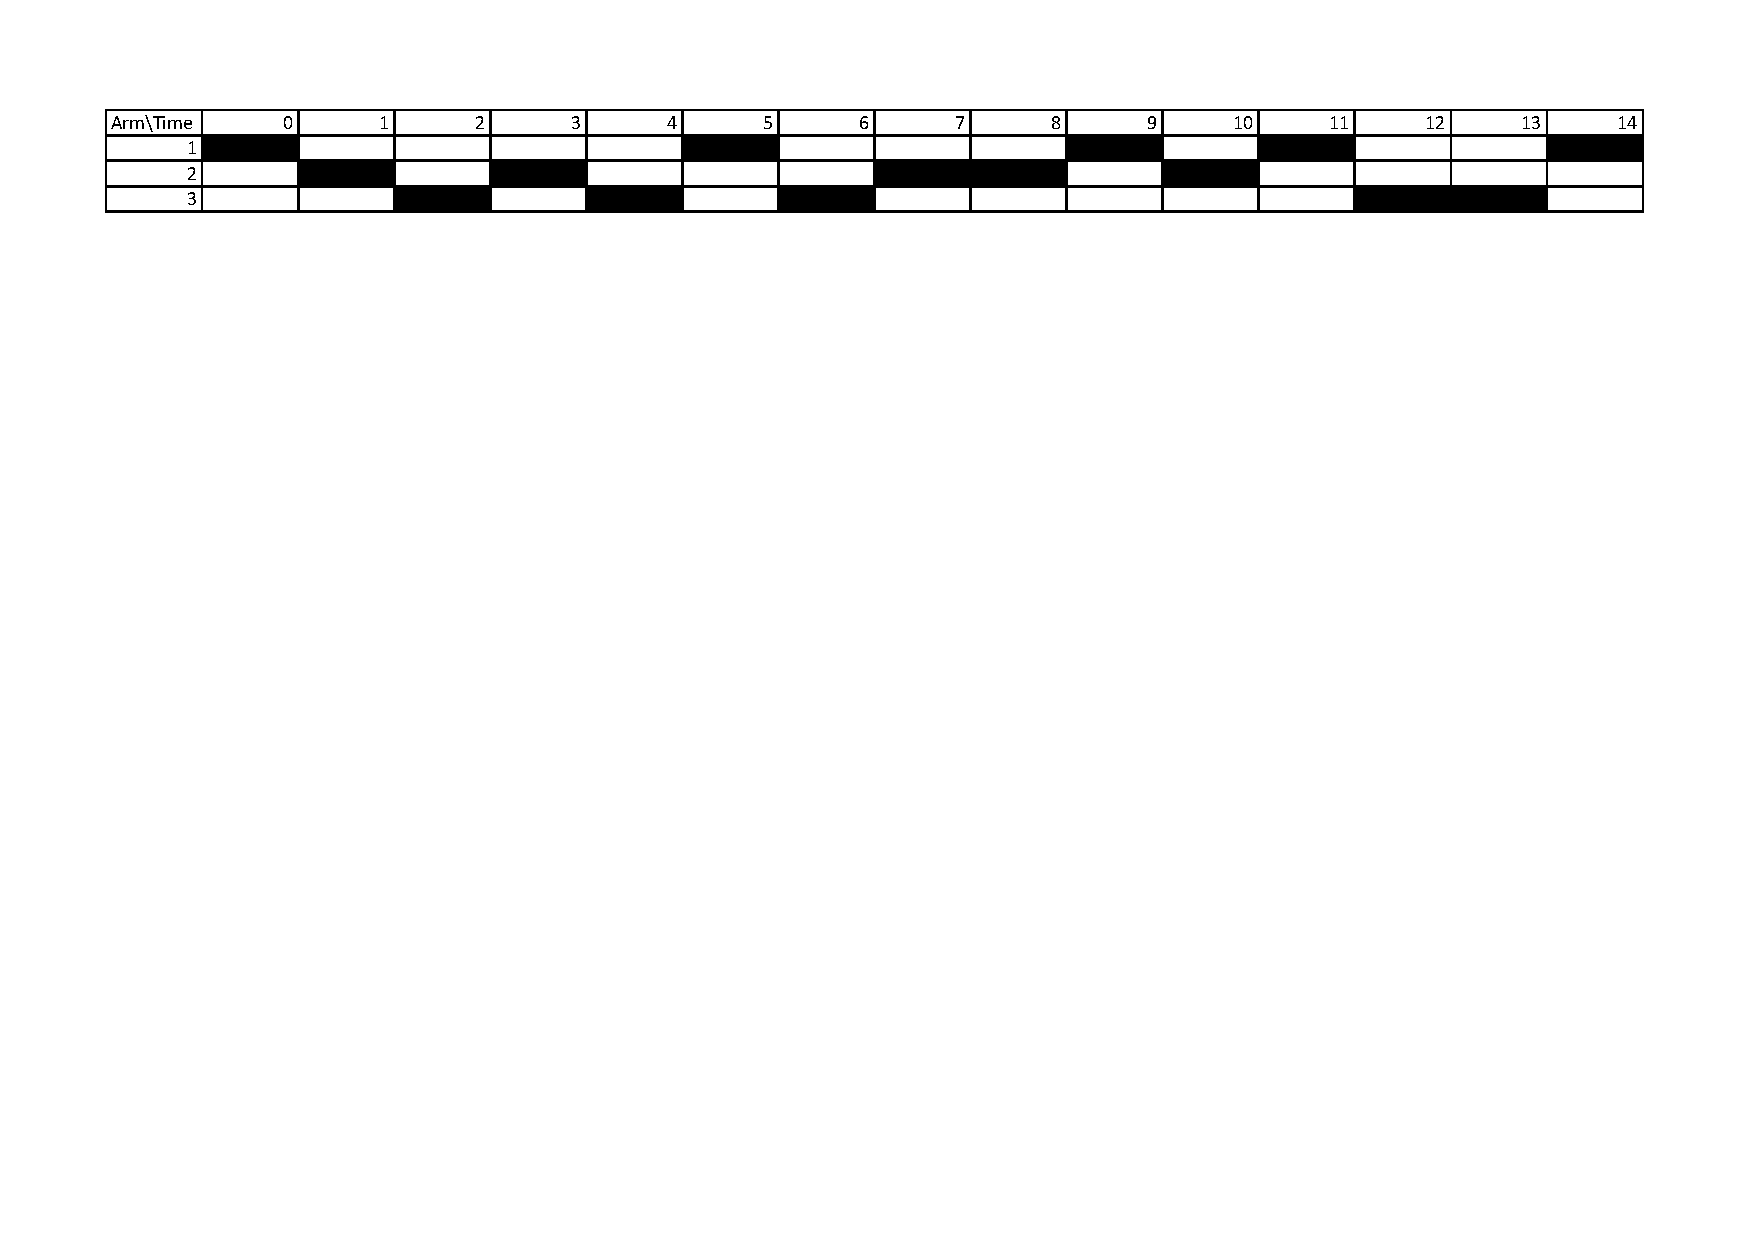
\includegraphics[width=\textwidth]{images/Sampling.pdf}
	\caption{A schematic representation of arm selections over time for $K=3$ arms. In this schematic, an arm selected at any given time is indicated by a black box. Note that arm $1$ is selected at time $t=0$, arm $2$ at time $t=1$ and arm $3$ at time $t=2$. Thereafter, for $t\geq 3$, arm $1$ is selected at certain time instants and is not selected at certain other time instants. Whenever arm $1$ is not selected, \emph{some} other arm is selected, as a consequence of which the delay of arm $1$ increases, and it is this fact that must be captured as a constraint on the delays of arm $1$. Similar constraints apply for each of the other arms.}
	\label{restless_with_known_fig:arm_selections}
\end{figure}

Assume without loss of generality that under the policy $\pi$, arm $a$ is selected at time $t=\tau(\pi)$. Then, it follows that 
\begin{equation}
	(a-1)+\sum\limits_{i\in\mathcal{S}}~\sum\limits_{d=1}^{\infty}~d\,N(\tau(\pi),d,i,a) + 1 = \tau(\pi)+1;\label{restless_with_known_eq:constraint}
\end{equation}
in \eqref{restless_with_known_eq:constraint}, the term $(a-1)$ on the left-hand side denotes the number of time instants that have passed before arm $a$ is selected for the first time. The second term on the left-hand side of \eqref{restless_with_known_eq:constraint} denotes the total number of time instants that have passed, starting from time $t=K$, until the final selection time instant of arm $a$. The last term on the left-hand side of \eqref{restless_with_known_eq:constraint} counts the final selection instant of arm $a$. Thus, the total value of the left-hand side of \eqref{restless_with_known_eq:constraint} is equal to the total number of time instants that have passed from $t=0$ to $t=\tau(\pi)$ (both inclusive), which is precisely the quantity on the right-hand side of \eqref{restless_with_known_eq:constraint}. Applying $E_h[\cdot]$ to both sides of \eqref{restless_with_known_eq:constraint}, and using the monotone convergence theorem, we arrive at the following relation after some rearrangement:
\begin{equation}
	\sum\limits_{i\in\mathcal{S}}~\sum\limits_{d=1}^{\infty} d~\frac{E_h[N(\tau(\pi),d,i,a)]}{E_h[\tau(\pi)]}+\frac{a-1}{E_h[\tau(\pi)]}=1.\label{restless_with_known_eq:constraint_1}
\end{equation}
In fact, it is easy to see that \eqref{restless_with_known_eq:constraint}, and therefore \eqref{restless_with_known_eq:constraint_1}, holds for every arm, whether or not the arm is selected at time $t=\tau(\pi)$. Mimicking the steps in Section \ref{restless_with_known_appndx:proof_of_prop_lower_bound}, and using  \eqref{restless_with_known_eq:equiv_of_lower_bound_2} in place of \eqref{restless_with_known_eq:lower_bound_2} in Section \ref{restless_with_known_appndx:proof_of_prop_lower_bound} along with the constraint in \eqref{restless_with_known_eq:constraint_1}, we arrive at the following relation in place of \eqref{restless_with_known_eq:lower_bound_5}:
\begin{align}
	d(\epsilon,1-\epsilon)&\leq \sup\limits_{\kappa}\,\min\limits_{h'\neq h}\bigg\lbrace E_h\left[\sum\limits_{a=1}^{K}\log\frac{P_h(X_{a-1}^{a})}{P_{h'}(X_{a-1}^{a})}\right]\nonumber\\
	&\hspace{1.5cm}+\bigg(E_h[\tau(\pi)-K+1]\bigg)\cdot\,\sum\limits_{a=1}^{K}~\sum\limits_{d=1}^{\infty}~\sum\limits_{i\in\mathcal{S}}\kappa(d,i,a)\, D((P_h^a)^{d}(\cdot|i)\|(P_{h'}^a)^{d}(\cdot|i))\bigg\rbrace,\label{restless_with_known_eq:equiv_lower_bound_5}
\end{align}
where $d(\epsilon, 1-\epsilon)$ is the relative entropy between a Bernoulli distribution with parameter $\epsilon$ and a Bernoulli distribution with parameter $1-\epsilon$, and the supremum in \eqref{restless_with_known_eq:equiv_lower_bound_5} is over all probability distributions $\kappa$ on $\{1,2,\ldots\}\times\mathcal{S}\times\mathcal{A}$ that satisfy the constraint
\begin{equation}
	\sum\limits_{i\in\mathcal{S}}~\sum\limits_{d=1}^{\infty} d~\kappa(d,i,a)=1\quad \text{ for all }a\in\mathcal{A}.\label{restless_with_known_eq:constraint_2}
\end{equation}
The constraint in \eqref{restless_with_known_eq:constraint_2} may be obtained from \eqref{restless_with_known_eq:constraint_1} by letting $E_h[\tau(\pi)]\to \infty$ (which is the same as $\epsilon\downarrow 0$) and replacing the fractional term on the left-hand side of \eqref{restless_with_known_eq:constraint_1} by $\kappa(d,i,a)$; here, $\kappa(d,i,a)$ represents the long-term joint probability of observing arm $a$ to have a delay $d$ and last observed state $i$, and subsequently selecting arm $a$. 

Dividing both sides of \eqref{restless_with_known_eq:equiv_lower_bound_5} by $d(\epsilon,1-\epsilon)$, and using the fact that $d(\epsilon,1-\epsilon)/\log(1/\epsilon)\to 1$ as $\epsilon\downarrow 0$, we arrive at
\begin{equation}
	\liminf\limits_{\epsilon\downarrow 0}\inf\limits_{\pi\in\Pi(\epsilon)}\frac{E_h[\tau(\pi)]}{\log(1/\epsilon)}\geq \frac{1}{R_1^*(P_1,P_2)},\label{restless_with_known_eq:lower_bound_equiv}
\end{equation}
where $R_1^*(P_1,P_2)$ is the {\color{black} value} of the following constrained optimisation problem:
\begin{align}
	&R_1^*(P_1,P_2)=\sup\limits_{\kappa}\,\min\limits_{h'\neq h}\,\sum\limits_{a=1}^{K}~\sum\limits_{d=1}^{\infty}~\sum\limits_{i\in\mathcal{S}}\kappa(d,i,a)\, D((P_h^a)^{d}(\cdot|i)\|(P_{h'}^a)^{d}(\cdot|i))\nonumber\\
	&\text{subject to}\nonumber\\
	&\hspace{1cm}\sum\limits_{i\in\mathcal{S}}~\sum\limits_{d=1}^{\infty} d~\kappa(d,i,a)=1\quad \text{ for all }a\in\mathcal{A},\nonumber\\
	&\hspace{1cm} \sum\limits_{d=1}^{\infty}~\sum\limits_{i\in\mathcal{S}}~\sum\limits_{a=1}^K \kappa(d,i,a)=1,\nonumber\\
	&\hspace{1cm} \kappa(d,i,a)\geq 0\quad\text{ for all }d\in\{1,2,\ldots\},~i\in\mathcal{S},~a\in\mathcal{A}.\label{restless_with_known_eq:constrained_LPP}
\end{align}
Notice that \eqref{restless_with_known_eq:constrained_LPP} constitutes an infinite-dimensional linear programming problem with linear constraints. {\color{black} It is not clear if there exists $\kappa$ that (a) satisfies the constraints in \eqref{restless_with_known_eq:constrained_LPP} and (b) attains the supremum in the expression for $R_1^*(P_1, P_2)$}. Also, it is not clear if the constraints in \eqref{restless_with_known_eq:constrained_LPP} constitute the tightest set of constraints. From Proposition \ref{restless_with_known_prop:lower_bound}, we must of course have $R_1^*(P_1,P_2)\geq R^*(P_1,P_2)$.

We end with a remark that by taking into account the delays and the last observed states of all the arms in deriving the lower bound, as done in Section \ref{restless_with_known_appndx:proof_of_prop_lower_bound}, the constraint in \eqref{restless_with_known_eq:constraint} is automatically captured since any vector $\underline{d}=(d_1,\ldots,d_K)$ of arm delays belongs, by definition, to the subset $\mathbb{S}$ which obeys the constraint in  \eqref{restless_with_known_eq:constraint}. Thus, the viewpoint of controlled Markov processes greatly simplifies the analysis of the lower bound. The key insight of this chapter is that our `lift' approach of considering the arm delays and the last observed states of all the arms jointly, instead of dealing with the delays and last observed states of each arm separately, makes the problem amenable to analysis.

\subsection{Restriction to SRS Class Suffices} \label{restless_with_known_appndx:an_important_theorem}
An important step in the derivation of the lower bound \eqref{restless_with_known_eq:lower_bound} presented in Section \ref{restless_with_known_appndx:proof_of_prop_lower_bound} is the replacement of the supremum over the set $\Pi(\epsilon)$ appearing in \eqref{restless_with_known_eq:lower_bound_5} to the set $\Pi_{\textsf{SRS}}$ of all SRS policies (compare the right hand side of \eqref{restless_with_known_eq:lower_bound_5} with that of \eqref{restless_with_known_eq:lower_bound_7}). Here, $\Pi(\epsilon)$, which the set of all policies whose probability of error at stoppage is at most $\epsilon$, may potentially include non-SRS policies too. The aforementioned step in the proof of the lower bound is possible thanks to the following theorem which is an analogue of \cite[Theorem 8.8.2]{puterman2014markov} for countable state space controlled Markov processes. We omit the proof of the theorem as it follows straightforwardly from the proof of \cite[Theorem 8.8.2]{puterman2014markov}. 

Recall that for each $\pi^\lambda\in \Pi_{\textsf{SRS}}$, the controlled Markov process $\{(\underline{d}(t), \underline{i}(t)):t\geq K\}$ is, in fact a Markov process. Furthermore, when the trembling hand parameter $\eta>0$, this Markov process is ergodic (Lemma \ref{restless_with_known_lem:pi_delta^lambda_is_an_SSRS}).
%We omit the proof since it follows along the lines of the proof of \cite[Theorem 8.8.2]{puterman2014markov}.
\begin{theorem} 
\label{restless_with_known_theorem:restriction_to_SRS_policies}
	\begin{enumerate}
		\item For each $\pi^\lambda\in \Pi_{\textsf{SRS}}$, $(\underline{d}, \underline{i})\in \mathbb{S}$ and $a\in \mathcal{A}$, let
			\begin{equation}
				\nu^\lambda(\underline{d}, \underline{i}, a) = \mu^\lambda(\underline{d}, \underline{i})~\left(\frac{\eta}{K} + (1-\eta) ~\lambda(a\mid \underline{d}, \underline{i})\right),
			\end{equation}
			where $\eta>0$ is the trembling hand parameter and $\mu^\lambda$ is the unique stationary distribution of the Markov process $\{(\underline{d}(t), \underline{i}(t)):t\geq K\}$ under the SRS policy $\pi^\lambda$. Then, $\nu^\lambda$ is a feasible  solution to \eqref{restless_with_known_eq:lower_bound_6_1}-\eqref{restless_with_known_eq:lower_bound_6_3}.
			
		\item Let $\nu$ be any feasible solution to \eqref{restless_with_known_eq:lower_bound_6_1}-\eqref{restless_with_known_eq:lower_bound_6_3}. Then, for each $(\underline{d}, \underline{i})\in \mathbb{S}$, $\sum\limits_{a=1}^{K} ~\nu(\underline{d}, \underline{i}, a) > 0$.
				Let $\lambda^*$ be such that
				$$
				\frac{\eta}{K}+(1-\eta)~\lambda^*(a\mid \underline{d}, \underline{i}) \coloneqq \frac{\nu(\underline{d}, \underline{i}, a)}{\sum\limits_{a=1}^{K} ~\nu(\underline{d}, \underline{i}, a)}, \quad (\underline{d}, \underline{i})\in \mathbb{S}, ~a\in \mathcal{A}.
				$$
				Then, $\nu^{\lambda^*}$ is a feasible solution to \eqref{restless_with_known_eq:lower_bound_6_1}-\eqref{restless_with_known_eq:lower_bound_6_3} and 
				$$
				\nu^{\lambda^*}(\underline{d}, \underline{i}, a)=\nu(\underline{d}, \underline{i}, a)\quad \text{for all }(\underline{d}, \underline{i})\in \mathbb{S}\text{ and }a\in \mathcal{A}.
				$$
	\end{enumerate}
\end{theorem}

\section{Summary}
\label{restless_with_known_sec:conclusions}
We make several concluding remarks in summary.
\begin{enumerate}
\item  From \eqref{restless_with_known_eq:main_result}, when the trembling hand parameter $\eta>0$, we see that
\begin{equation}
	\lim\limits_{\epsilon\downarrow 0} ~ \inf\limits_{\pi\in\Pi(\epsilon)} ~ \frac{E_h[\tau(\pi)]}{\log(1/\epsilon)} = \frac{1}{R_\eta^*(P_1,P_2)}.\label{restless_with_known_eq:final-result}
\end{equation}
We have thus provided an answer to \eqref{restless_with_known_eqn:objective} on the minimum growth rate of the expected time to identify the odd arm location as $\epsilon \downarrow 0$.

\item The asymptotically optimal $\lambda(\cdot|\cdot)$ in the restless case may depend on the history unlike that in the prior works \cite{Vaidhiyan2017, vaidhiyan2012active, vaidhiyan2017learning, prabhu2017optimal} where $\lambda(\cdot)$ did not depend on history, even in the rested Markov case. At first glance, this is surprising for the rested Markov case, but in retrospect, these features are apparent from an examination of the optimisation problem \eqref{restless_with_known_eq:R_delta^*(h,P_1,P_2)} in these special cases. 

\item Computability of $R_\eta^*(P_1,P_2)$ may be an issue, and one must usually resort to $Q$-learning for restless Markov arms \cite{avrachenkov2020whittle} to arrive at good policies. The fact that $D(P_k^{d_a} (\cdot | i_a) || P_l^{d_a} (\cdot | i_a))$, $k,l\in\{1,2\}$, converges as $d_a \rightarrow \infty$ could enable restriction of the countable state space $\mathbb{S}$ to a finite set, and could lead to good approximations.

%\item Consider the optimisation problem \eqref{restless_with_known_eq:R_delta^*(h,P_1,P_2)}. For a fixed $h' \neq h$, we used results from \cite{fleming2012stochastic, borkar1988control} to establish existence of policies that attain the supremum. The ideas here can be extended to establish existence of policies that attain the supremum and satisfy the inequality in \eqref{restless_with_known_eq:structure_on_lambda_restless_arms}  with an equality. The finite nature of the number of alternative arms could lead to some simplifications. This is a direction that remains open for exploration.

\item When the trembling hand parameter $\eta>0$, the ergodicity of the Markov process $(\underline{d}(t), \underline{i}(t))$ under any SRS policy ensures that time averages approach the ensemble averages. This is crucial to show achievability. Note also the use of uniqueness of the stationary distribution to show the converse. The trembling hand model may be viewed as a {\em regularisation} that gives stability of the aforementioned Markov process for free. If the trembling hand parameter $\eta$ were 0, one could deliberately add some regularisation parameterised by $\eta$, and let this parameter $\eta \downarrow 0$. $R_{0}^*(P_1,P_2)$ governs the lower bound, whereas $\lim\limits_{\eta \downarrow 0}R_{\eta}^*(P_1,P_2)$ governs the upper bound. The resulting lower and upper bounds on the growth rate may have a gap.

%\item Open questions: The key difficulties when $\eta=0$ are (a) absence of ergodicity property, and (b) a formal verification of the envelope theorem. 
%%and (c) a verification of tightness of stationary distributions. 
%It would be interesting to study these. Another interesting setting to study is when $P_1$ and $P_2$ are unknown and have to be learnt along the way, which forms the subject of the next chapter.
\end{enumerate}


















